%%%%%%%%%%%%%%%%%%%%%%%%%%%%%%%%%%%%%%%%%%%%%%%
%%%     Declarations (skip to Begin Document, line 88, for parts you fill in)
%%%%%%%%%%%%%%%%%%%%%%%%%%%%%%%%%%%%%%%%%%%%%%%

%%\documentclass[10pt]{article}
%%\documentclass[10pt]{report}
\documentclass[letterpaper]{article}
\usepackage{geometry}
%\usepackage{xcolor}
\usepackage[table]{xcolor}
\usepackage{amsmath}
\usepackage[some]{background}
%\usepackage{lipsum}
%\usepackage{natbib}
\usepackage{siunitx}

% C I T A T I O N S
\usepackage[backend=biber, style=apa]{biblatex}  
%\usepackage{biblatex} 
\addbibresource{paperpile.bib}

\usepackage[hidelinks]{hyperref}

% C A P T I O N S
%\usepackage{caption, copyrightbox}
%\captionsetup{justification=centering, labelfont=sc, labelsep=endash}

% Tables
\usepackage{float}
\usepackage[utf8]{inputenc}
\usepackage{tabularx}
\usepackage{booktabs}
\usepackage{longtable}

\usepackage{diagbox} %table split headers
\usepackage{longtable}
\usepackage{array}
\usepackage{rotating}
\usepackage{eqparbox}
\usepackage{makecell, caption, booktabs}
\usepackage{wrapfig}
\usepackage{colortbl}

% Stuff needed to get table to span pages
\usepackage{enumitem}
%\usepackage{array, booktabs, longtable}
\newcolumntype{x}[1]{>{\raggedright}p{#1}}
% Highlight a column
\definecolor{Highlight}{HTML}{FFF59C}
\newcolumntype{h}{>{\columncolor{Highlight}}c}


\usepackage{etoolbox}
\AtBeginEnvironment{longtable}{%
    \setlist[itemize]{nosep,     % <-- new list setup
                      topsep     = 0pt       ,
                      partopsep  = 0pt       ,
                      leftmargin = *         ,
                      label      = $\bullet$ ,
                      before     = \vspace{-\baselineskip},
                      after      = \vspace{-0.5\baselineskip}
                        }
                           }% end of AtBeginEnvironment
% End table span
% Listings
\usepackage{listings}

\usepackage{geometry}  % Lots of layout options.  See http://en.wikibooks.org/wiki/LaTeX/Page_Layout
\geometry{letterpaper}  % ... or a4paper or a5paper or ... 
\usepackage{fullpage}  % somewhat standardized smaller margins (around an inch)
\usepackage{setspace}  % control line spacing in latex documents
\usepackage[parfill]{parskip}  % Activate to begin paragraphs with an empty line rather than an indent

\usepackage{amsmath,amssymb}  % latex math
\usepackage{empheq} % http://www.ctan.org/pkg/empheq
\usepackage{bm,upgreek}  % allows you to write bold greek letters (upper & lower case)

% for typsetting algorithm pseudocode see http://en.wikibooks.org/wiki/LaTeX/Algorithms_and_Pseudocode
\usepackage{algorithmic,algorithm}  

\usepackage{graphicx}  % inclusion of graphics; see: http://en.wikibooks.org/wiki/LaTeX/Importing_Graphics
% allow easy inclusion of .tif, .png graphics
\DeclareGraphicsRule{.tif}{png}{.png}{`convert #1 `dirname #1`/`basename #1 .tif`.png}

% \usepackage{subfigure}  % allows subfigures in figure
\usepackage{caption}
\usepackage{subcaption}

\usepackage{xspace}
\newcommand{\latex}{\LaTeX\xspace}

\usepackage{color}  % http://en.wikibooks.org/wiki/LaTeX/Colors

\long\def\todo#1{{\color{red}{\bf TODO: #1}}}

\long\def\ans#1{{\color{blue}{\em #1}}}
\long\def\ansnem#1{{\color{blue}#1}}
\long\def\boldred#1{{\color{red}{\bf #1}}}
\long\def\boldred#1{\textcolor{red}{\bf #1}}
\long\def\boldblue#1{\textcolor{blue}{\bf #1}}

% Useful package for syntax highlighting of specific code (such as python) -- see below
\usepackage{listings}  % http://en.wikibooks.org/wiki/LaTeX/Packages/Listings
\usepackage{textcomp}


%%% The following lines set up using the listings package
\renewcommand{\lstlistlistingname}{Code Listings}
\renewcommand{\lstlistingname}{Code Listing}

%%% Specific for python listings
\definecolor{gray}{gray}{0.5}
\definecolor{green}{rgb}{0,0.5,0}

\lstnewenvironment{python}[1][]{
\lstset{
language=python,
basicstyle=\footnotesize,  % could also use this -- a little larger \ttfamily\small\setstretch{1},
stringstyle=\color{red},
showstringspaces=false,
alsoletter={1234567890},
otherkeywords={\ , \}, \{},
keywordstyle=\color{blue},
emph={access,and,break,class,continue,def,del,elif ,else,%
except,exec,finally,for,from,global,if,import,in,i s,%
lambda,not,or,pass,print,raise,return,try,while},
emphstyle=\color{black}\bfseries,
emph={[2]True, False, None, self},
emphstyle=[2]\color{green},
emph={[3]from, import, as},
emphstyle=[3]\color{blue},
upquote=true,
morecomment=[s]{"""}{"""},
commentstyle=\color{gray}\slshape,
emph={[4]1, 2, 3, 4, 5, 6, 7, 8, 9, 0},
emphstyle=[4]\color{blue},
literate=*{:}{{\textcolor{blue}:}}{1}%
{=}{{\textcolor{blue}=}}{1}%
{-}{{\textcolor{blue}-}}{1}%
{+}{{\textcolor{blue}+}}{1}%
{*}{{\textcolor{blue}*}}{1}%
{!}{{\textcolor{blue}!}}{1}%
{(}{{\textcolor{blue}(}}{1}%
{)}{{\textcolor{blue})}}{1}%
{[}{{\textcolor{blue}[}}{1}%
{]}{{\textcolor{blue}]}}{1}%
{<}{{\textcolor{blue}<}}{1}%
{>}{{\textcolor{blue}>}}{1},%
%framexleftmargin=1mm, framextopmargin=1mm, frame=shadowbox, rulesepcolor=\color{blue},#1
framexleftmargin=1mm, framextopmargin=1mm, frame=single,#1
}}{}
%%% End python code listing definitions

\DeclareMathOperator{\diag}{diag}
\DeclareMathOperator{\cov}{cov}


%\bibliography{./paperpile.bib}
\author{Evan McGinnis}
\title{Automated Weeding}



\definecolor{titlepagecolor}{cmyk}{1,.60,0,.40}

\DeclareFixedFont{\bigsf}{T1}{phv}{b}{n}{1.5cm}

\backgroundsetup{
scale=1,
angle=0,
opacity=1,
contents={\begin{tikzpicture}[remember picture,overlay]
 \path [fill=titlepagecolor] (-0.5\paperwidth,5) rectangle (0.5\paperwidth,10);  
\end{tikzpicture}}
}
\makeatletter                       
\def\printauthor{%                  
    {\large \@author}}              
\makeatother
\author{%
    Evan McGinnis \\
    Graduate Student \\
    Biosystems Analytics \\
    \texttt{evanmc@arizona.edu}\vspace{40pt} \\
    }
\begin{document}
\begin{titlepage}
\BgThispage
\newgeometry{left=1cm,right=4cm}
\vspace*{1cm}
\noindent
%%\vspace*{0.4\textheight}
\textcolor{white}{\Huge\textbf{\textsf{Weed Classification in Row Crops}}}
\vspace*{3.5cm}\par
\noindent
\begin{minipage}{0.35\linewidth}
    \begin{flushright}
        \printauthor
    \end{flushright}
\end{minipage} \hspace{15pt}
%
\begin{minipage}{0.02\linewidth}
    \rule{1pt}{175pt}
\end{minipage} \hspace{-10pt}
%
\begin{minipage}{0.70\linewidth}
\vspace{5pt}
    \begin{abstract} 
The precision treatment of weeds within a crop depends first on accurate classification of plants into two classes: desired plants and undesired plants. This paper presents the findings that weeds and crop can be distinguished from each other using shape, color, texture, and placement, all factors that can be extracted from RGB images. The shape factors found to be significant were the length to width ratio, and the shape index. The color factor found to be significant was the mean Y value in the YIQ color space. The placement factor found to be significant was the distance the plant was from the crop-line. Using these factors in classification resulted in the correct classification rate of weeds at 100\%, but an incorrect classification rate of crop as weeds of 6.9\% using logistic regression.
    \end{abstract}
\end{minipage}
\end{titlepage}
\restoregeometry
%
% F R O N T  M A T T E R
%
\tableofcontents
\listoffigures
\listoftables
%\listofequations
\newpage

%
% O V E R V I E W 
%



\section{Introduction}
While precision treatment of unwanted vegetation may be the end-product, classifying vegetation in the acquired images is the first major step in that workflow. This paper concentrates on the binary classification of vegetation into two discrete classes: desired vegetation (lettuce crop) and undesired vegetation (weeds and crop occupying an undesired position). Once classified, vegetation can be treated using a variety of mechanical, chemical~(\cite{Saile2022-vu}), or no-touch~(\cite{Saile2022-vu,Mwitta2022-yt}) methods. The specifics of and integration with the treatment system are beyond the scope of this document, but treatment considerations will be discussed within the context of establishing a buffer zone around desired vegetation to minimize crop damage.

 While it is tempting to use the terms \textit{weed} and \textit{crop} (and this document will often use those terms), this proposal will more often reference vegetation as \textit{desired} (crop in the position wanted) and \textit{undesired} (weeds and crop not in the position wanted).  That is, classification more often answers the question ``do we want this plant'' than ``is this plant a weed''. These two questions are often conflated, but are subtly distinct.

 Images from UAVs offer several advantages over those obtained with manned aircraft and satellite, such as the economics or flexibility of acquisition, but this study will leverage the relative ease with which UAVs are able to gather imagery from various distances close to the ground. While many studies use images gathered close to the ground from a single distance and report classification accuracy and others use images gathered at multiple distances, reporting (the inevitably declining) accuracy seen with increasing distance, the former tends to suffer when the same attributes are applied at higher distances and the latter from holding the set of attributes constant as altitudes increase. \citeauthor{Ong2023-lm}, in a study of classification of Chinese Cabbage, classifies vegetation acquired at an average of 2m AGL using a single set of attributes, Local Binary Pattern (LBP, a texture descriptor), and a single approach (Random Forest) leveraging those attributes, validating the use of texture in classification \parencite{Ong2023-lm}. \citeauthor{Etienne2021-ik}, in a study of Corn and Soybean plots, used imagery gathered from both 10m and 30m AGL. but found that the best training set for selected algorithm (YOLOv3) was taken from the set of images acquired from 10m \parencite{Etienne2021-ik}. The parameters selected as significant to classification fall into three basic categories: shape, color, and texture. Variants of each of these categories will be used in this study. 
In a study of weed mapping in sunflower crop, \citeauthor{Perez-Ortiz2015-yk} present findings from images taken from three distances AGL, 30m, 60m, and 100m, classifying each pixel as crop, weed, or soil using SVM, KNN, and k-means (and variants of those) approaches \parencite{Perez-Ortiz2015-yk}. While this approach does indeed yield weed maps that lend themselves to later study, the approach is a bit different in terms of what is being classified. In that study, individual pixels are being classified, in contrast to this study that seeks to classify individual plants.
In a study of weeds in corn, \citeauthor{Lin2017-xq} used shape metrics as part of the classification workflow, stressing the importance of expressing shape metrics that are not rotationally variant. More importantly, the study details a shape metric possessing the desired qualities for use in classification. Using shape and texture (GLCM), the study demonstrated an overall accuracy exceeding 95\%.\footnote{\citeauthor{Lin2017-xq}'s study did not report some items that are of interest: the distances of the imagery to the camera, and the false positive rate of weed identification. While the high overall rate sounds is certainly impressive, that metric will not be used in this study. Additionally, the images of vegetation were acquired under controlled conditions, something that is not reproducible in the field an at higher distances AGL.} \citeauthor{Sabzi2020-af}, in a study of a potato field, used various channels of color spaces (YIQ, YCbCr, HSI) as well as texture (Grey-Level Co-occurrence Matrix, GLCM) to achieve a high correct classification rate, but the use of GLCM is not applied  to channels of the color conversion, only to RGB images that have been converted to greyscale \parencite{Sabzi2020-af}. While this is a conventional use of the texture identification technique, it does not leverage the information content available in other color spaces.



\section{Data Preparation}
Data for this study comes in two forms: static images obtained with visible light cameras and prepared images of manually manipulated scenarios.  Feature analysis and machine learning use unmanipulated images exclusively, while tests will be conducted on a mixture of the two.

\subsection{Discrete Static Images}
Discrete image sets are those acquired in the field with a hand-held RGB camera. The image set used in this analysis was acquired by hand using a Samsung SM-G930V. These images are not without problems, of course. As images often have vegetation at the edges of the image, and frequently of only a single plant, attempts to classify vegetation considering shape and position within the crop-line can lead to poor results. As Figure~\ref{fig:problem-cropline} shows, a crop-line cannot be determined or surmised using only a single crop image. In this instance, the crop-line is assumed to be along the center-line of the image. Figure~\ref{fig:problem-cutoff} demonstrates the problem encountered where the shape of an object cannot be used as a factor in classification, as the shape is distorted by having a regular, straight edge.

% Side by side subfigures 
\begin{figure}[H]
	\begin{subfigure}[h]{0.48\linewidth}
		\includegraphics[width=1\linewidth]{./figures/problem-cropline.jpg}
		\caption{The crop-line cannot be determined.}
		\label{fig:problem-cropline}
		
	\end{subfigure}
	\hfill
	\begin{subfigure}[h]{0.48\linewidth}
		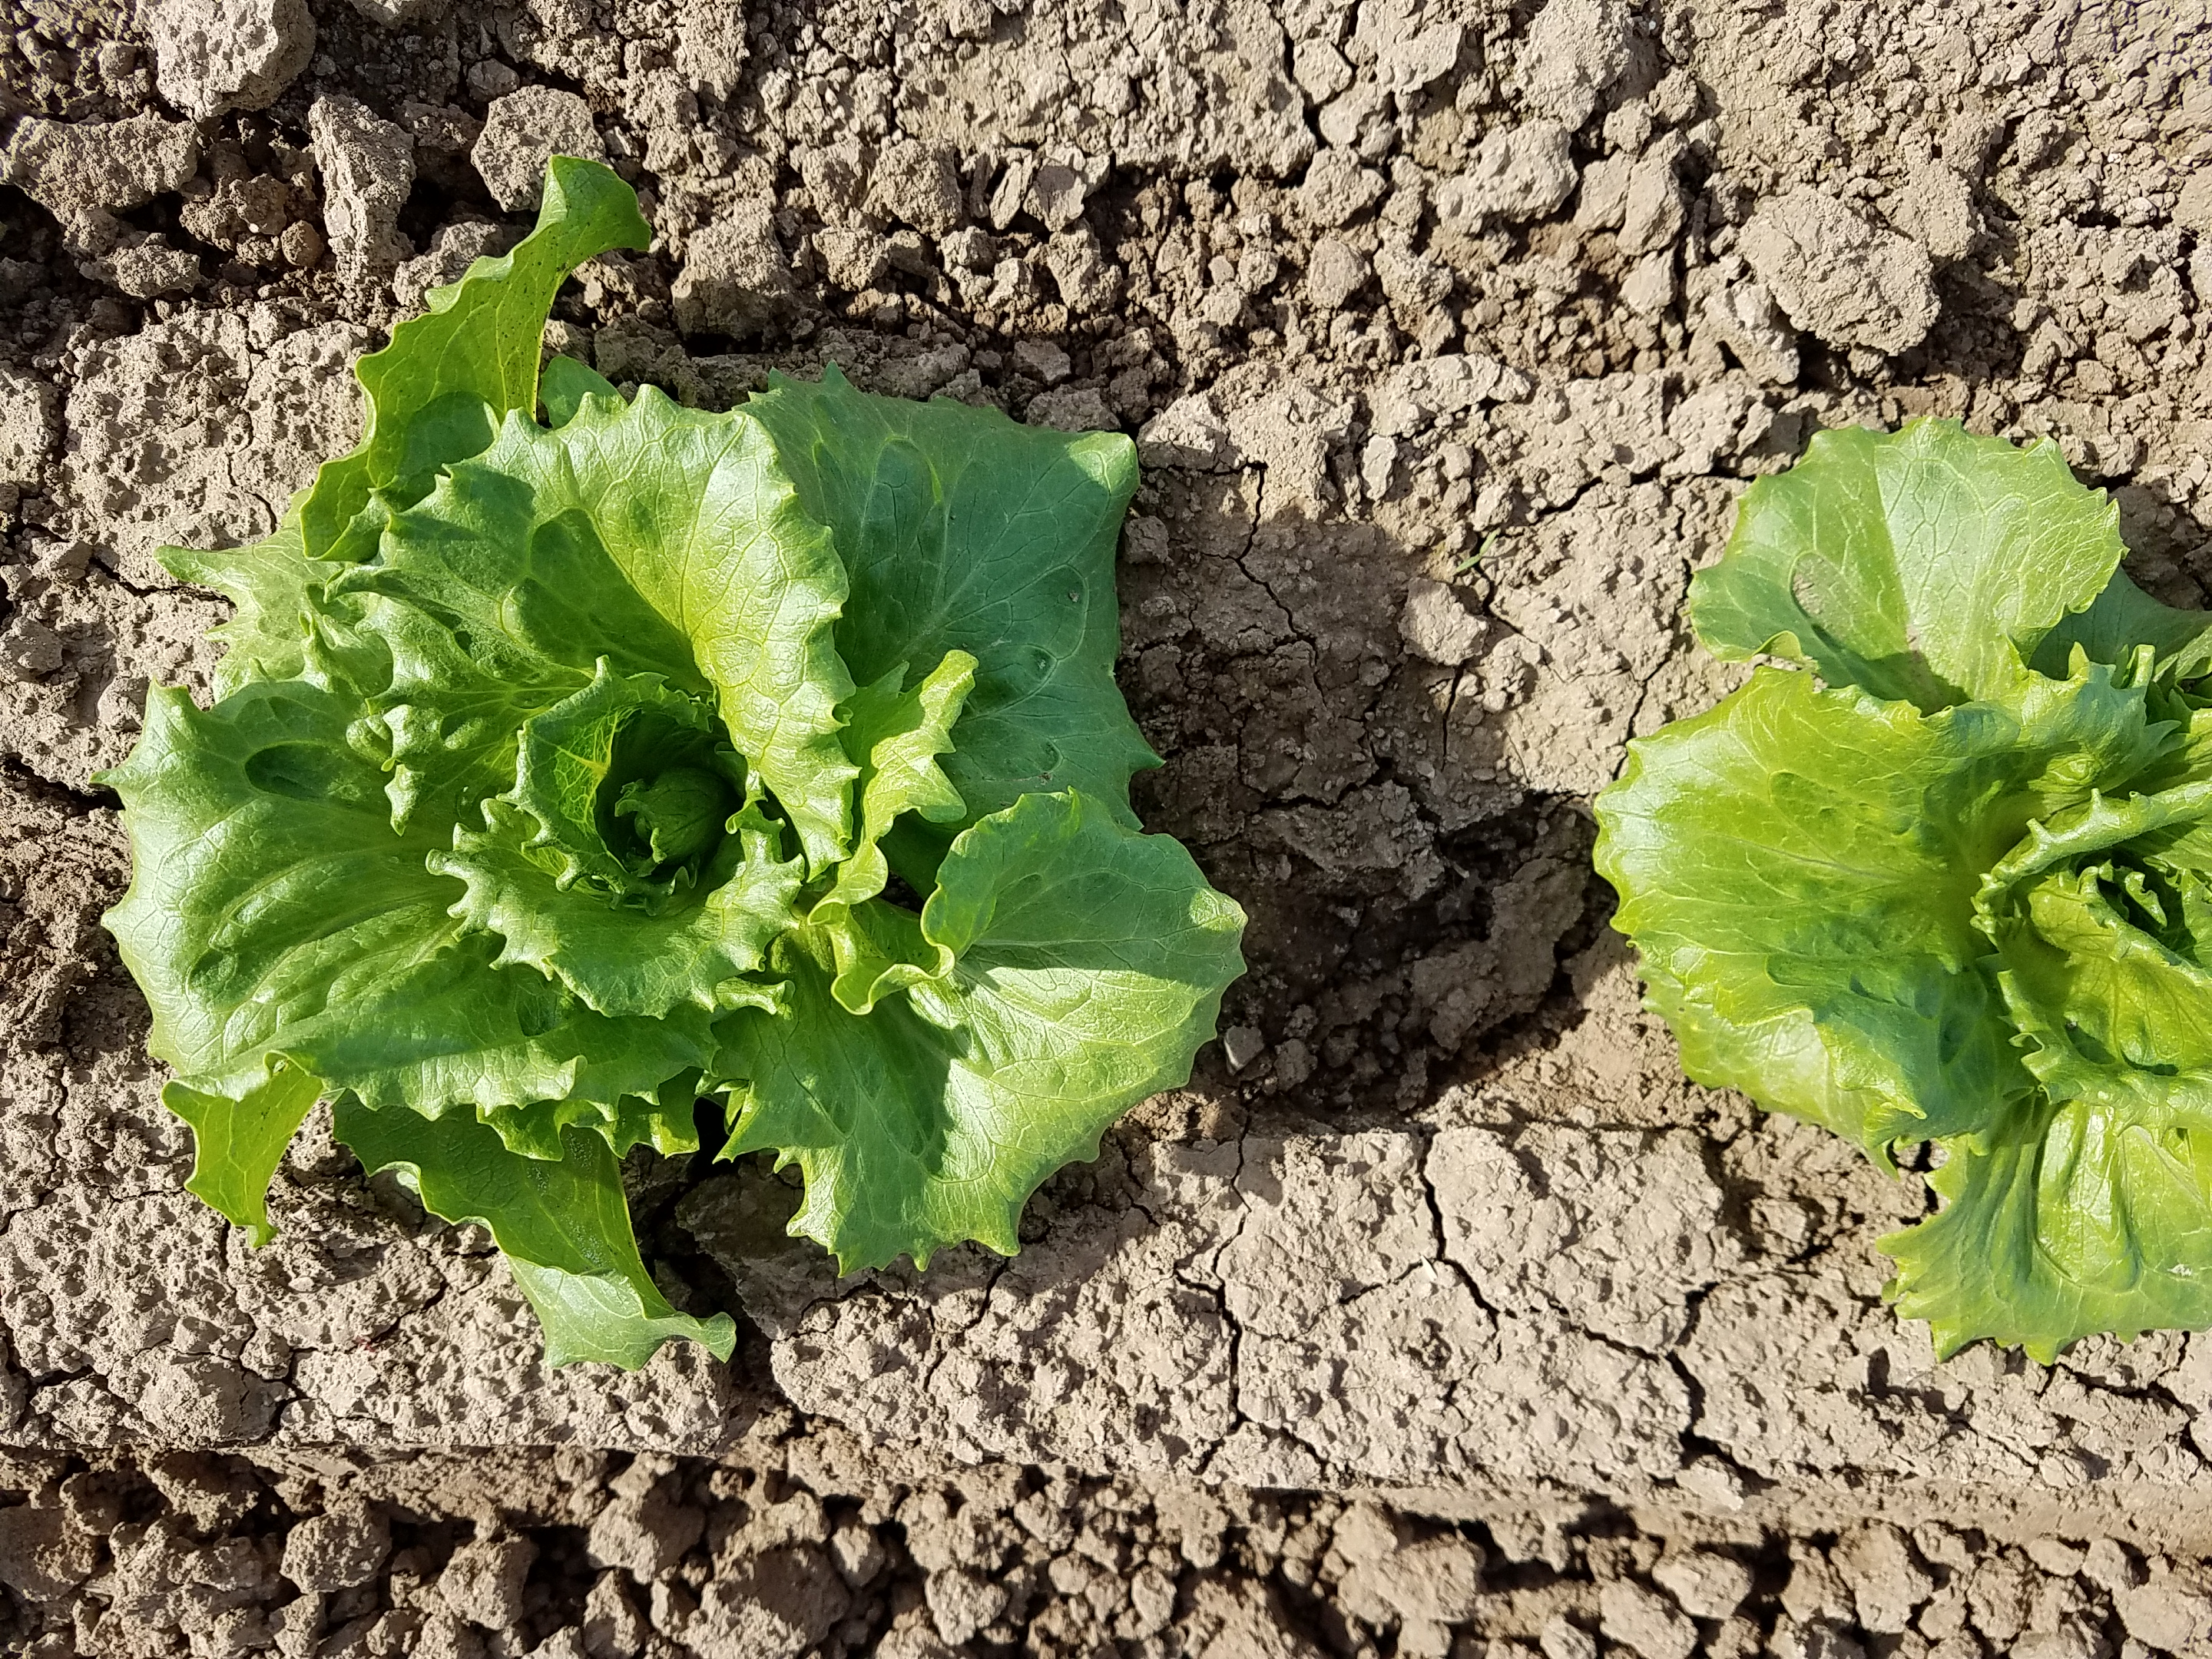
\includegraphics[width=1\linewidth]{./figures/problem-cutoff.jpg}
		\caption{The vegetation is cut off.}
		\label{fig:problem-cutoff}		
	\end{subfigure}%
	\caption[Common problems in field images]{These cases illustrate common problems encountered in image sets where the crop-line cannot be conclusively determined (\ref{fig:problem-cropline}) and the cutoff of vegetation (\ref{fig:problem-cutoff}). In the case where images contain a single image of crop the intended crop-line cannot be automatically determined. In the case where vegetation is cut off along the edges of the image shape analysis cannot be used, as otherwise the shape of the vegetation is distorted by the clean, straight edge. \\ \textit{Images source: Dr.~Mark Siemens, University of Arizona}}
\end{figure}



\subsection{Prepared Images}
The images acquired in the field are prepared using Adobe Photoshop\textsuperscript{\textregistered} to create test data for various scenarios:
\begin{itemize}
	\item{Rows of vegetation requiring thinning. This is the case where vegetation that would otherwise be classified as \textit{desired} is instead classified as \textit{undesired}, as its placement within the crop-line violates a placement rule. Typically, this would be the case where crop required thinning to achieve the minimum distance between plants.} This is achieved by duplicating an existing plant in the image and choosing a placement that will achieve that scenario.
	\item{Unwanted vegetation too close to wanted vegetation. This is the case where vegetation is identified as \textit{undesired}, but is left untreated due to the risk of treatment would pose to the crop.} This is achieved in two ways -- duplicating or moving an existing weed within the image and inserting a new weed image obtained elsewhere.
	\item{Debris in the image -- this is the case where non-vegetated matter appears in the image.}
\end{itemize}

\begin{figure}[H]
	\begin{subfigure}[h]{0.48\linewidth}
		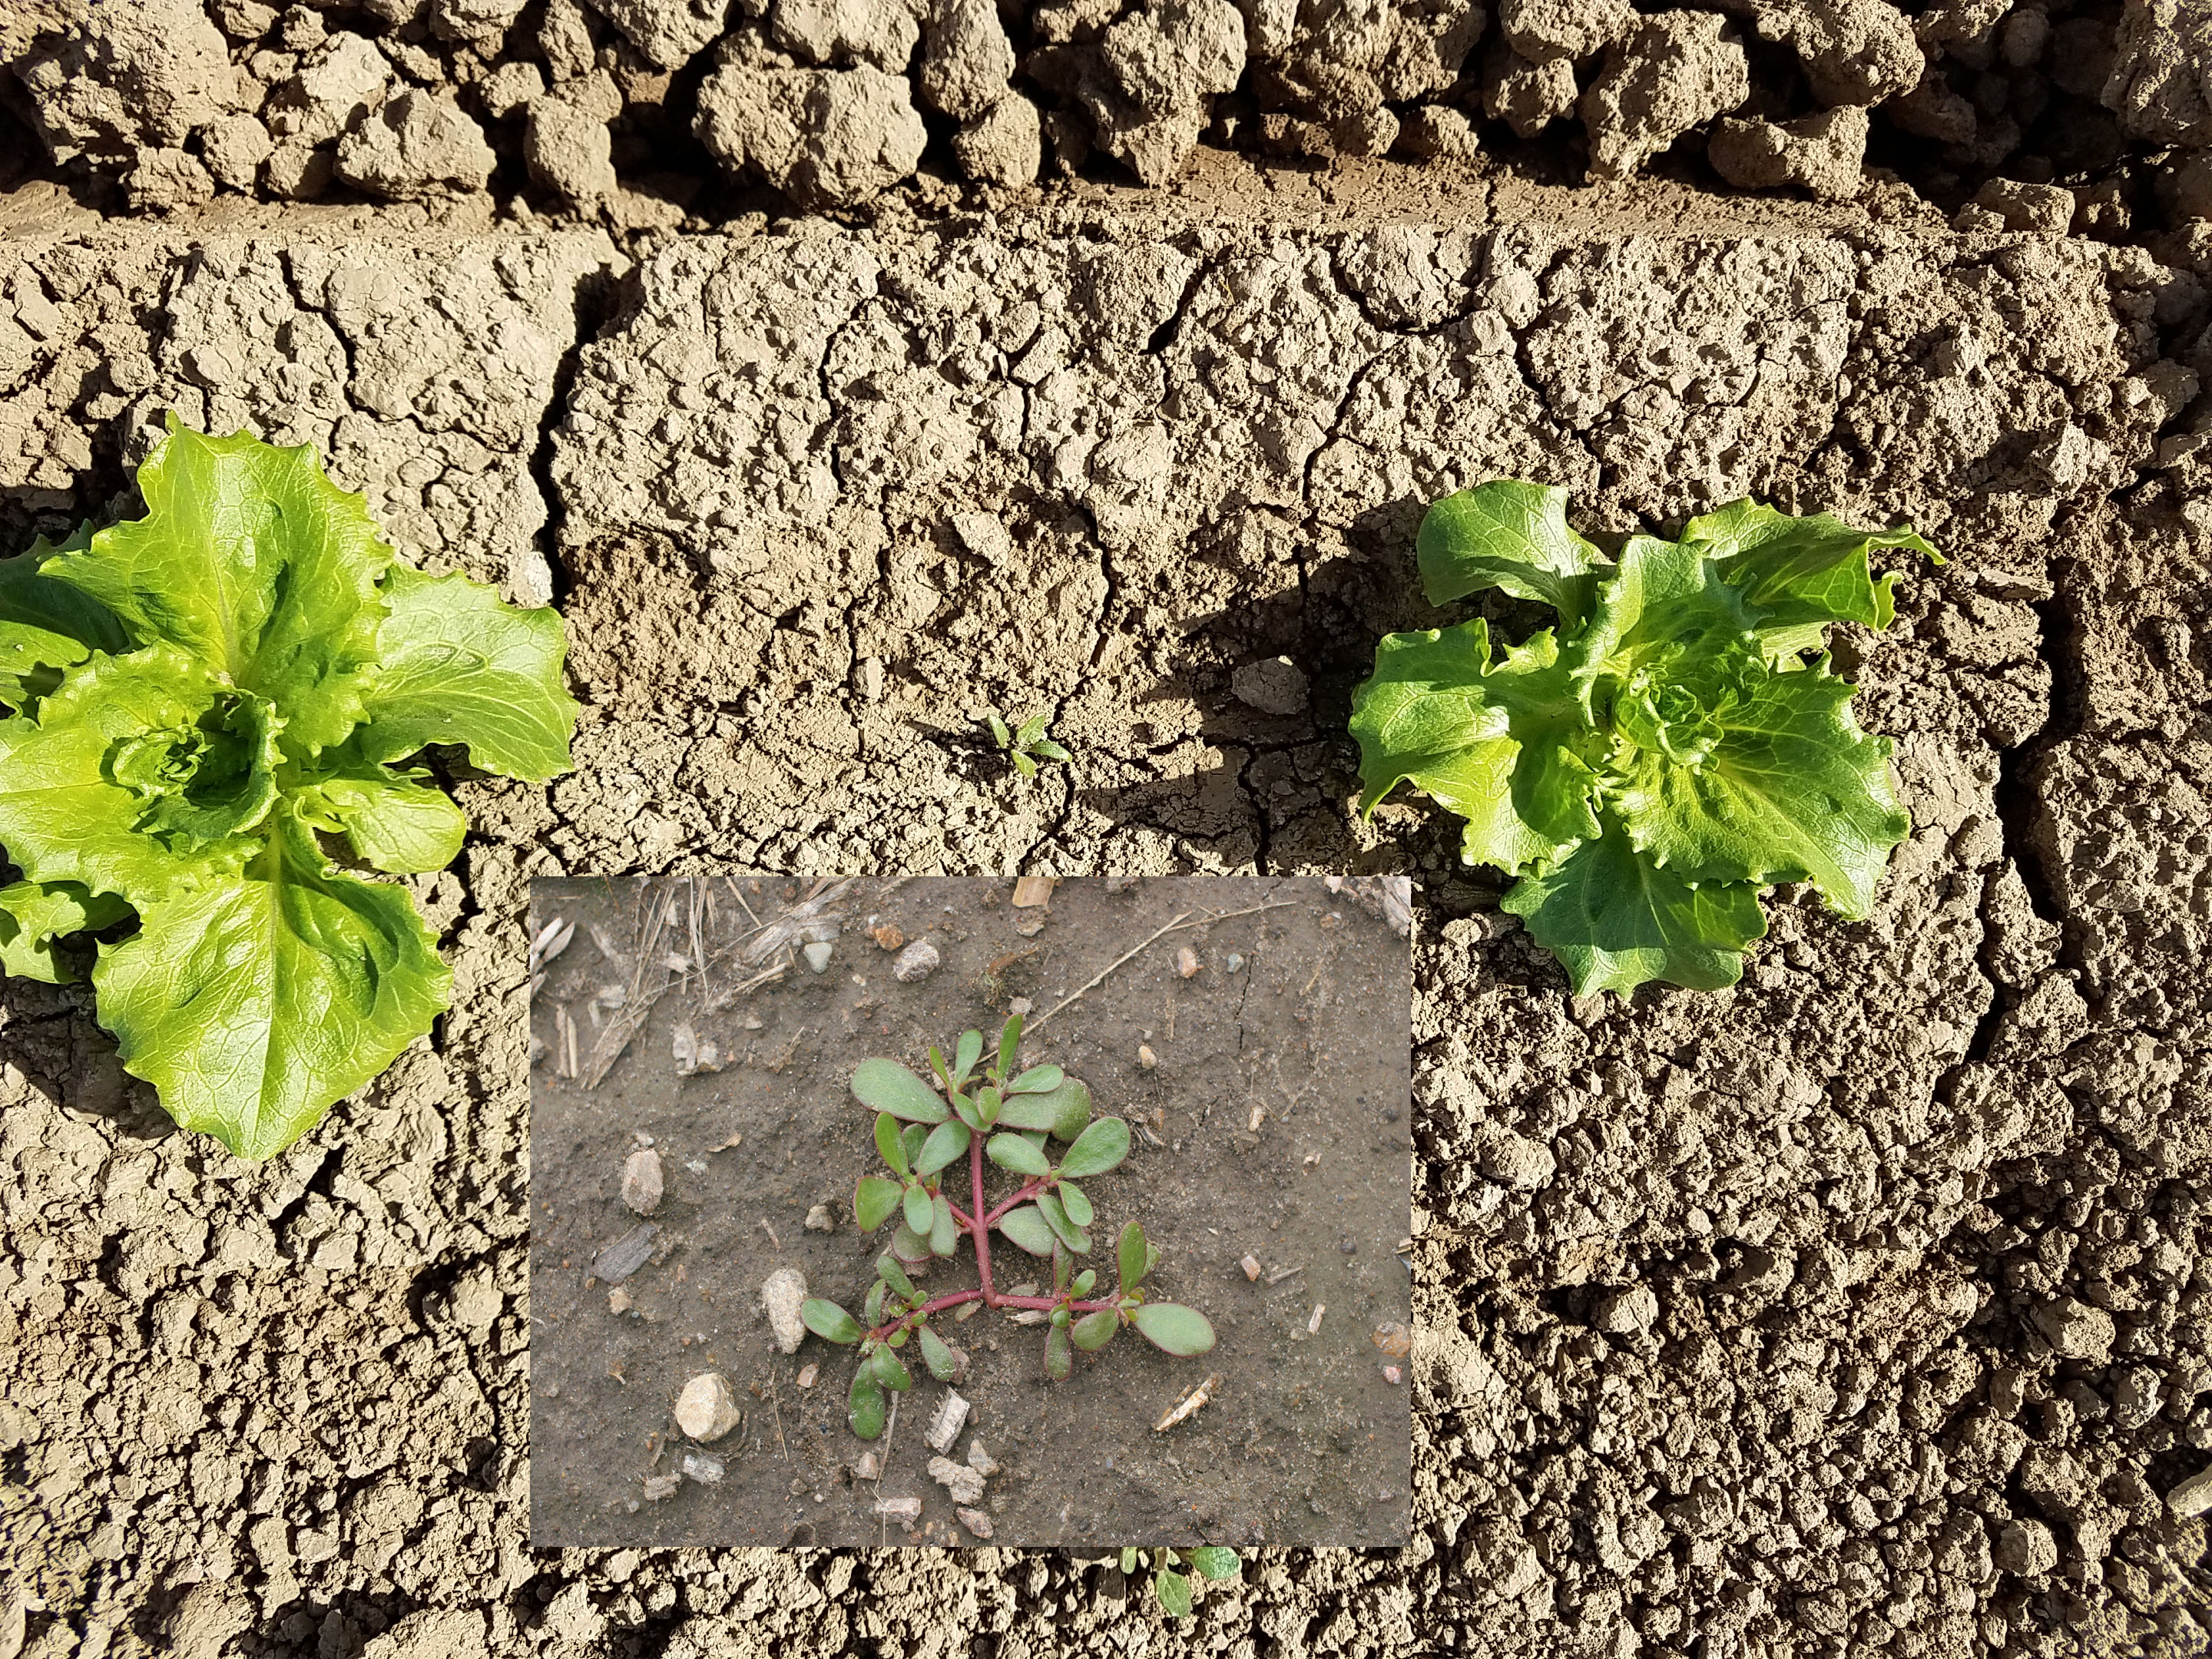
\includegraphics[width=1\linewidth]{./figures/with-purslane.jpg}
		\caption{Purslane (\textit Portulaca oleracea) inserted into the image.}
		\label{fig:prepared-weed}
	\end{subfigure}
	\hfill
	\begin{subfigure}[h]{0.48\linewidth}
		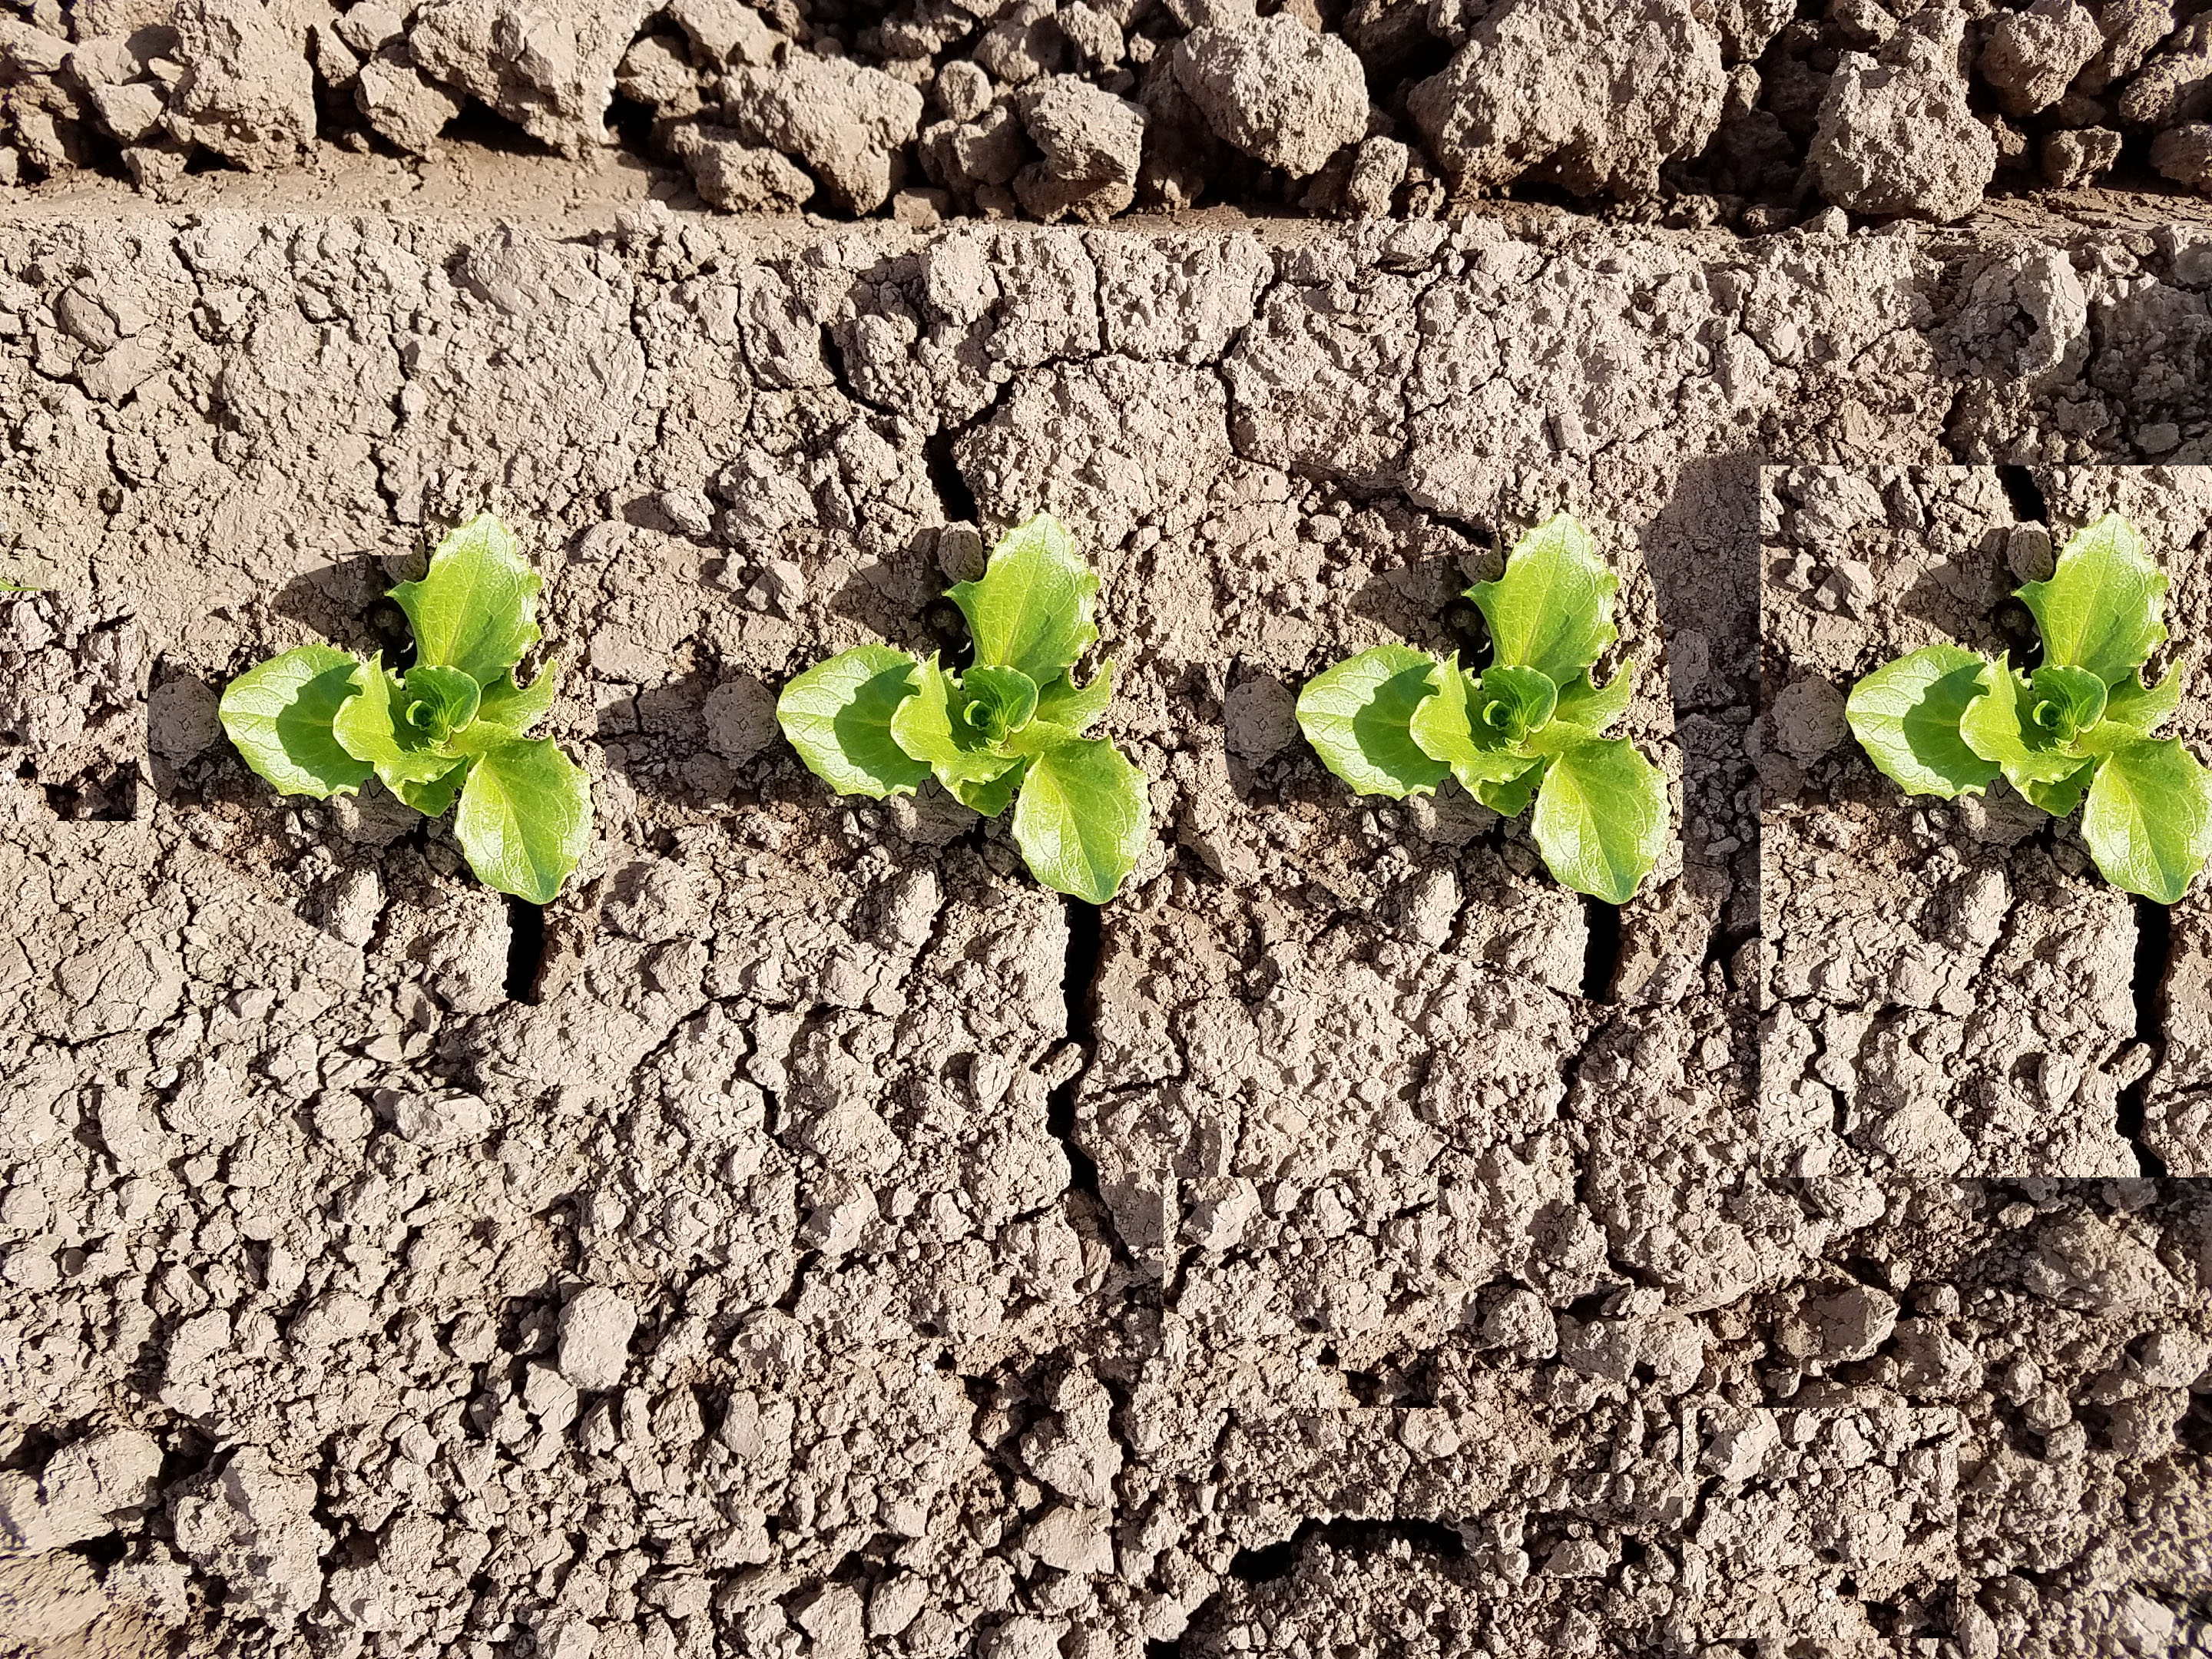
\includegraphics[width=1\linewidth]{./figures/thinning.jpg}
		\caption{Crop is replicated.}
		\label{fig:prepared-thinning}		
	\end{subfigure}%
	\caption[Prepared images]{Images acquired in the field are subsequently manipulated by either inserting images of weeds not already present (\ref{fig:prepared-weed}), or portions of the same image (\ref{fig:prepared-thinning}). Both cases are intended to present situations that should be handled by the classification algorithms. \\ \textit{Manipulated images of originals from Dr. Mark Siemens, University of Arizona}}
\end{figure}


Here, vegetation is placed within separate layers to create a composite image that shows the desired result. In Figure~\ref{fig:prepared-thinning}, a single lettuce plant is replicated several times to form an image that appears to be that of several plants. Notice the obvious seam in the lettuce plant on the right hand side of the image. As these pixels will be discarded early in image processing, they will have no effect on the current process as a whole, but may be a consideration if future processing considers factors such as the vegetation’s shadow.



\section{Approach To Classification}
The goal of this processing flow is to determine what each item within the image is and classify it as desired or undesired. Weeds are, of course, undesired, but crop plants can also be classified as \textit{undesired} in the case of thinning operations, so this document will use the term \textit{undesired} and \textit{weed} interchangeably. Vegetation in an image falls into one of these classifications:
\begin{itemize}
	\item{Desired, the crop}
	\item{Undesired, either crop that must be thinned or weeds that can be treated without crop damage}
	\item{Unknown, vegetation that cannot be confidently identified}
	\item{Ignored, vegetation that is too close to desired vegetation to be treated without crop damage}
\end{itemize}

Additionally, this work makes a few simplifying assumptions about the images:
\begin{itemize}
	\item{The crop line is approximately in the middle of the image.}
	\item{Crop is typically in roughly horizontal alignment (the centers will be with a few degrees of each other).}
	\item{Weed centers are typically not in horizontal alignment.}
	\item{Crop is typically much larger than weeds.}
\end{itemize}

These are not without exceptions. For instance, a weed may be in perfect aligment within a crop line and two other plants. Each of these observations, however, are used in classification. Take, for instance, the observation that crop tends to be much larger than weeds. If the size of an item is three times that of another, the smaller item is -- more likely than not -- a weed.

\section {Study Area}
This study will be carried out at the University of Arizona Maricopa Agricultural Center (MAC) on a cantaloupe crop overseen by Drs. Attalah and Elshikha (University of Arizona), as part of another study.\footnote{The field in question is located at N 33.061805$^{\circ}$ W 111.966162$^{\circ}$} That study will involve three separate water treatments: center-pivot, flood irrigation, and drip. As the drip treatment study area is unlikely to produce a heavy weed load, it will not be included in this study, as differentiating between crop and weeds is an initial goal of this study. The study site is relatively free of obstacles that would impact low level flight with one notable exception: the center pivot irrigation system. Allowances will be made to avoid that system, but doing so is not expected to affect flight plans, as images in only subset of the field is planned to be captured.
 

\section{Software Environment \& Source code}
Both commercial and open-source software were used in the development an operational aspects of this study. While the majority of the software (the operational portions responsible for image processing and classification) was written in Python, commercial packages were used for pre-processing. Additionally, R was used in visualization and analysis of classification results. Some of these components play a large enough role that they warrant special mention in various places throughout this document, but in-depth descriptions of them will not be made here. Likewise, this list is not exhaustive, as numerous libraries were used for a few functions, but included here. The complete source code for this project is available in this GitHub repository: \href{https://github.com/evan-mcginnis/weeds}{\textit {weeds}}. Images, both raw and processed, are far too large to be hosted with GitHub, and are available on request from the author.

All development was done on Windows 10 and Ubuntu 18.04.06 with analysis on the University of Arizona's \textit{High Performance Compute Cluster}.

{
% This avoids the document line spacing affecting the contents of the table
\setstretch{1.0}
\begin{longtable}{x{\dimexpr.20\columnwidth-2\tabcolsep}
                  x{\dimexpr.20\columnwidth-2\tabcolsep}
                  x{\dimexpr.5\columnwidth-2\tabcolsep}}
%\begin{hyphenrules}{nohyphenation}
    \caption{Software Used}\label{tab:software}  \\
\toprule
{\textbf{Component}} & {\textbf{Use}} & {\textbf{Comment}}
\tabularnewline
\midrule
    \endfirsthead
%%%%
    \caption{Software Used (cont.)}\label{tab:software}  \\
\toprule
{\textbf{Component}} & {\textbf{Use}} & {\textbf{Comment}}
\tabularnewline
\midrule
    \endhead
%%%%
\midrule[\heavyrulewidth]
\multicolumn{3}{r}{\footnotesize\itshape
                   Continued on the next page}
    \endfoot
%%%%
\bottomrule
    \endlastfoot
%%%%
		PyCharm 
		& Python IDE     
		& Commercial software for Python development
\tabularnewline\addlinespace
		Python 3.9     
		& Python runtime                    
		& Most software was written in python
\tabularnewline\addlinespace
		scikit-learn
		& Machine Learning     
		& Implementations for various ML techniques 
\tabularnewline\addlinespace
		OpenCV2 
		& Image Processing     
		& Machine Vision and Image Processing framework
\tabularnewline\addlinespace
		Numpy
		& Numeric Processing   
		& Python library
\tabularnewline\addlinespace
		Pandas 
		& Numeric Processing     
		& Python library
\tabularnewline\addlinespace
		PyQT5 
		& UI     
		& User Interface Framework for Python
\tabularnewline\addlinespace
		R 
		& Post Processing     
		& Statistical Software
\tabularnewline\addlinespace
		Plotly
		& Visualization     
		& Graphing libraries
\tabularnewline\addlinespace
		Adobe Lightroom
		& Color Correction     
		& Commercial software used for pre-processing
\tabularnewline\addlinespace
		Dronelink
		& UAV Control     
		& Commercial software used for planning \& control
\tabularnewline\addlinespace
		MongoDB
		& Image organization     
		& No-SQL database 
\tabularnewline\addlinespace
		Docker Container
		& Virtualization     
		& Virtual containers host database and web server
\tabularnewline\addlinespace
		Slurm
		& Workload     
		& Supercomputer workload management
\tabularnewline\addlinespace
		NGINX
		& Web Server     
		& Host HTTP API requests
\label{table:software}
\end{longtable}
}

\section{Workflow}
Images are processed following the workflow shown in Figure~\ref{fig:workflow}. Each step in this workflow will be discussed in subsequent sections.\footnote{The example images and analysis within the next few sections are taken from a set of images supplied by Dr. Mark Siemens, University of Arizona, and as such are not expected to provide an exact match to those acquired under field conditions. These images, however, are useful in the demonstration of key techniques that will be applied to images gathered under field conditions. This image set of 39 images was taken in 2019 with a Samsung SM-G930V phone.}
\begin{figure}[H]
	\centering
	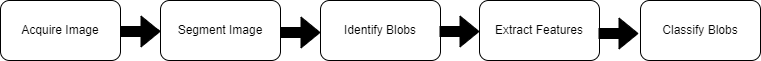
\includegraphics[width=1\linewidth]{./figures/workflow.drawio.png}
	\caption{Image processing workflow.}
	\label{fig:workflow}	
\end{figure}


\section{Acquire Image}
While the the processing step consists only of reading images from disk, actual acquisition was carried out in this study using a \href{https://www.dji.com/air-2s/specs} {DJI Mavic Air 2 SE} drone with a 20 MP camera, followed by color correction of acquired images. Each image acquisition was accompanied by an image of a \href{https://www.datacolor.com/spyder/products/spyder-checkr-photo/} {SpyderChecker 24} color calibration chart (under the same ambient lighting conditions) and color correction was subsequently applied using Adobe Photoshop Lightroom Classic and custom calibration profiles created using the Spyder Checkr software. Raw sensor data was stored in Adobe Digital Negative (DNG) format before color correction and conversion to a compressed JPG format for the resulting images. Images were color corrected against images taken before each flight of a Spyder CHECKR24 calibration target. The digital negative of each image (DNG, a standard format for raw sensor data) was corrected and converted to JPG format for subsequent processing.\footnote{The merits of raw, uncompressed, and unprocessed sensor data versus compressed, processed formats like JPG are beyond the scope of this document, but it is fair to say taking raw sensor data, processing, and then producing a compressed JPG is precisely what consumer products like phone cameras do. So that the color correction step can be inserted, the process of producing an image that can be viewed with most software is altered a bit, but essentially unchanged. A picture stored as a DNG is not higher resolution or higher quality than a JPG equivalent, just more easily manipulated without the introduction of errors} The sensor data for each image was quite large, requiring 38.5 MB of storage, resulting in these requirements for the altitudes studied:

Images were color corrected against images taken before each flight of a Spyder CHECKR24 calibration target. The digital negative of each image (DNG, a standard format for raw sensor data) was corrected and converted to JPG format for subsequent processing.\footnote{The merits of raw, uncompressed, and unprocessed sensor data versus compressed, processed formats like JPG are beyond the scope of this document, but it is fair to say taking raw sensor data, processing, and then producing a compressed JPG is precisely what consumer products like phone cameras do. So that the color correction step can be inserted, the process of producing an image that can be viewed with most software is altered a bit, but essentially unchanged.}
Where feasible, missions were conducted in the same ambient light conditions, but an exact match of ambient conditions using uncontrolled lighting is not always possible.


{\renewcommand{\arraystretch}{2}%

{
% This avoids the document line spacing affecting the contents of the table
\setstretch{1.0}
\begin{longtable}{x{\dimexpr.25\columnwidth-2\tabcolsep}
                  x{\dimexpr.35\columnwidth-2\tabcolsep}
                  x{\dimexpr.4\columnwidth-2\tabcolsep}}
%\begin{hyphenrules}{nohyphenation}
    \caption{Storage Requirements}\label{tab:storage}  \\
\toprule
{\textbf{AGL (meters)}} & {\textbf{DNG (Raw Sensor Data, MB)}} & {\textbf{Compressed (JPG, MB)}}
\tabularnewline
\midrule
    \endfirsthead
%%%%
    \caption{Storage Requirements (cont.)}\label{tab:storage}  \\
\toprule
{\textbf{AGL (meters)}} & {\textbf{DNG (Raw Sensor Data, MB)}} & {\textbf{Compressed (JPG, MB)}}
\tabularnewline
\midrule
    \endhead
%%%%
\midrule[\heavyrulewidth]
\multicolumn{3}{r}{\footnotesize\itshape
                   Continued on the next page}
    \endfoot
%%%%
\bottomrule
    \endlastfoot
%%%%
		2
		& XXX     
		& XXX
\tabularnewline\addlinespace
		5     
		& XXX                    
		& XXX
%\tabularnewline\addlinespace
\label{table:segmentation}
\end{longtable}
}

%
% I M A G E  S E G M E N T A T I O N
%
\section{Segment Image}
Perhaps the least compute-intensive portion of this workflow is simply to discard to portion of an image that does not contribute meaningfully to classification, and for this problem space those pixels that do not contribute useful information are, most notably, pixels representing the ground.
The portions of the images that did not contain pixels with vegetation present were the discarded by applying a visible light vegetation index to both isolate the vegetation and reduce the information content. This discards both the ground and debris while retaining the vegetation. These images were segmented using various visible light indices (\cite{Hunt2013-ih}, \cite{Hamuda2016-dw}). As this process is not the primary subject of this paper, it will be given only superficial mention here.  Various approaches to image segmentation are  summarized in Table \ref{table:segmentation}.  The intent of this step of the workflow is not to classify the individual plants, but to preprocess the image before further analysis is done.

{\renewcommand{\arraystretch}{2}%

{
% This avoids the document line spacing affecting the contents of the table
\setstretch{1.0}
% Example to span two pages
\begin{longtable}{x{\dimexpr.25\columnwidth-2\tabcolsep}
                  x{\dimexpr.35\columnwidth-2\tabcolsep}
                  x{\dimexpr.4\columnwidth-2\tabcolsep}}
%\begin{hyphenrules}{nohyphenation}
    \caption{Visible light indices}\label{tab:example}  \\
\toprule
{\textbf{Index}} & {\textbf{Formula}} & {\textbf{Comment}}
\tabularnewline
\midrule
    \endfirsthead
%%%%
    \caption{Visible light indices (cont.)}\label{tab:example}  \\
\toprule
{\textbf{Index}} & {\textbf{Formula}} & {\textbf{Comment}}
\tabularnewline
\midrule
    \endhead
%%%%
\midrule[\heavyrulewidth]
\multicolumn{3}{r}{\footnotesize\itshape
                   Continued on the next page}
    \endfoot
%%%%
\bottomrule
    \endlastfoot
%%%%
		Triangular Greenness
		& \begin{minipage}[t]{0.3\textwidth}
			$R_{green} - \alpha R_{red} - \beta R_{blue}\\ \alpha = \frac {2(\lambda_{blue} - \lambda_{green})} {(\lambda_{blue} - \lambda_{red})}\\ 
		    	\beta = \frac {2(\lambda_{green} - \lambda_{red})} {(\lambda_{blue} - \lambda_{red})} $
		   \end{minipage}     
		& Corrects for camera calibration using the peak sensitivity
\tabularnewline\addlinespace

		Normalized Difference     
		& $128 * \left( \left( \frac {(G - R)} {(G + R)} \right) + 1 \right) $                    
		& The NDI index produces a near-binary image. 
\tabularnewline\addlinespace

		Excess Green      
		& \begin{minipage}[t]{0.3\textwidth}
			$R = \frac {R} {R_{max}}\\ G = \frac {G} {G_{max}}\\ B = \frac {B} {B_{max}}$ 
		   \end{minipage}
		& ExG provided a clear contrast between plants and soil 
\tabularnewline\addlinespace

		Excess Red      
		& $1.3 R - G$ 
		& inspired by the fact that there are 4\% blue, and 32\% green, compared with 64\% red cones in the retina of the human eye
\tabularnewline\addlinespace

		Color Index of Vegetation Extraction      
		& $0.441 R - 0.811 G + 0.385 B + 18.78745$
		& This method was proposed to separate green plants from soil background in order to evaluate the crop growing status.
\tabularnewline\addlinespace

		Excess Green - Excess Red   
		& $ExG - ExR$ 
		& ExG used to extract the plant region and ExR used to eliminate the background noise (soil and residue) where green–red material (stems, branches, or petioles) may exist
\tabularnewline\addlinespace

		Normalized Green-Red Difference    
		& $\frac {(G - R)} {(G + R)}$ 
		& The method of NGRDI was used to overcome the differences in exposure settings selected by the digital camera when acquiring aerial photography of the field. 
\tabularnewline\addlinespace

		Vegetative Index      
		& $\frac {G} {R^aB^{(1-a)}}, a = 0.667$ 
		& VEG has a significant advantage because it is robust to lighting change.
\tabularnewline\addlinespace

		Com1   
		& $ExG + CIVE + ExGR + VEG$ 
		& High computational cost --- does not perform well in high or low light levels
\tabularnewline\addlinespace

		Modified Excess Green      
		& $1.262G - 0.884R = 0.311B$ 
		& Does not perform well in high or low light levels. 
\tabularnewline\addlinespace

		Combined Indices 2      
		& $0.36ExG + 0.47CIVE + 0.17VEG$ 
		& Uses weighting factors to emphasize strengths of various approaches
%\tabularnewline\addlinespace
\label{table:segmentation}
\end{longtable}
}

These indices are used to create a mask that is then applied to the original source image to permit vegetation to show while masking details that are not relevant (ground pixels, stones, and other items that may appear in field conditions) The intent here is to remove all pixels that are not relevant to the task of distinguishing between crop and weed while leaving the vegetated pixels unmanipulated.

\begin{figure}[H]
	\centering
	\begin{subfigure}[h]{.30\textwidth}
	  \centering
	  \includegraphics[width=1\linewidth]{figures/original.jpg}
	  \caption{Field view of lettuce and weed}
	  \label{fig:original}
	\end{subfigure}
	\begin{subfigure}[h]{.30\textwidth}
	  \centering
	  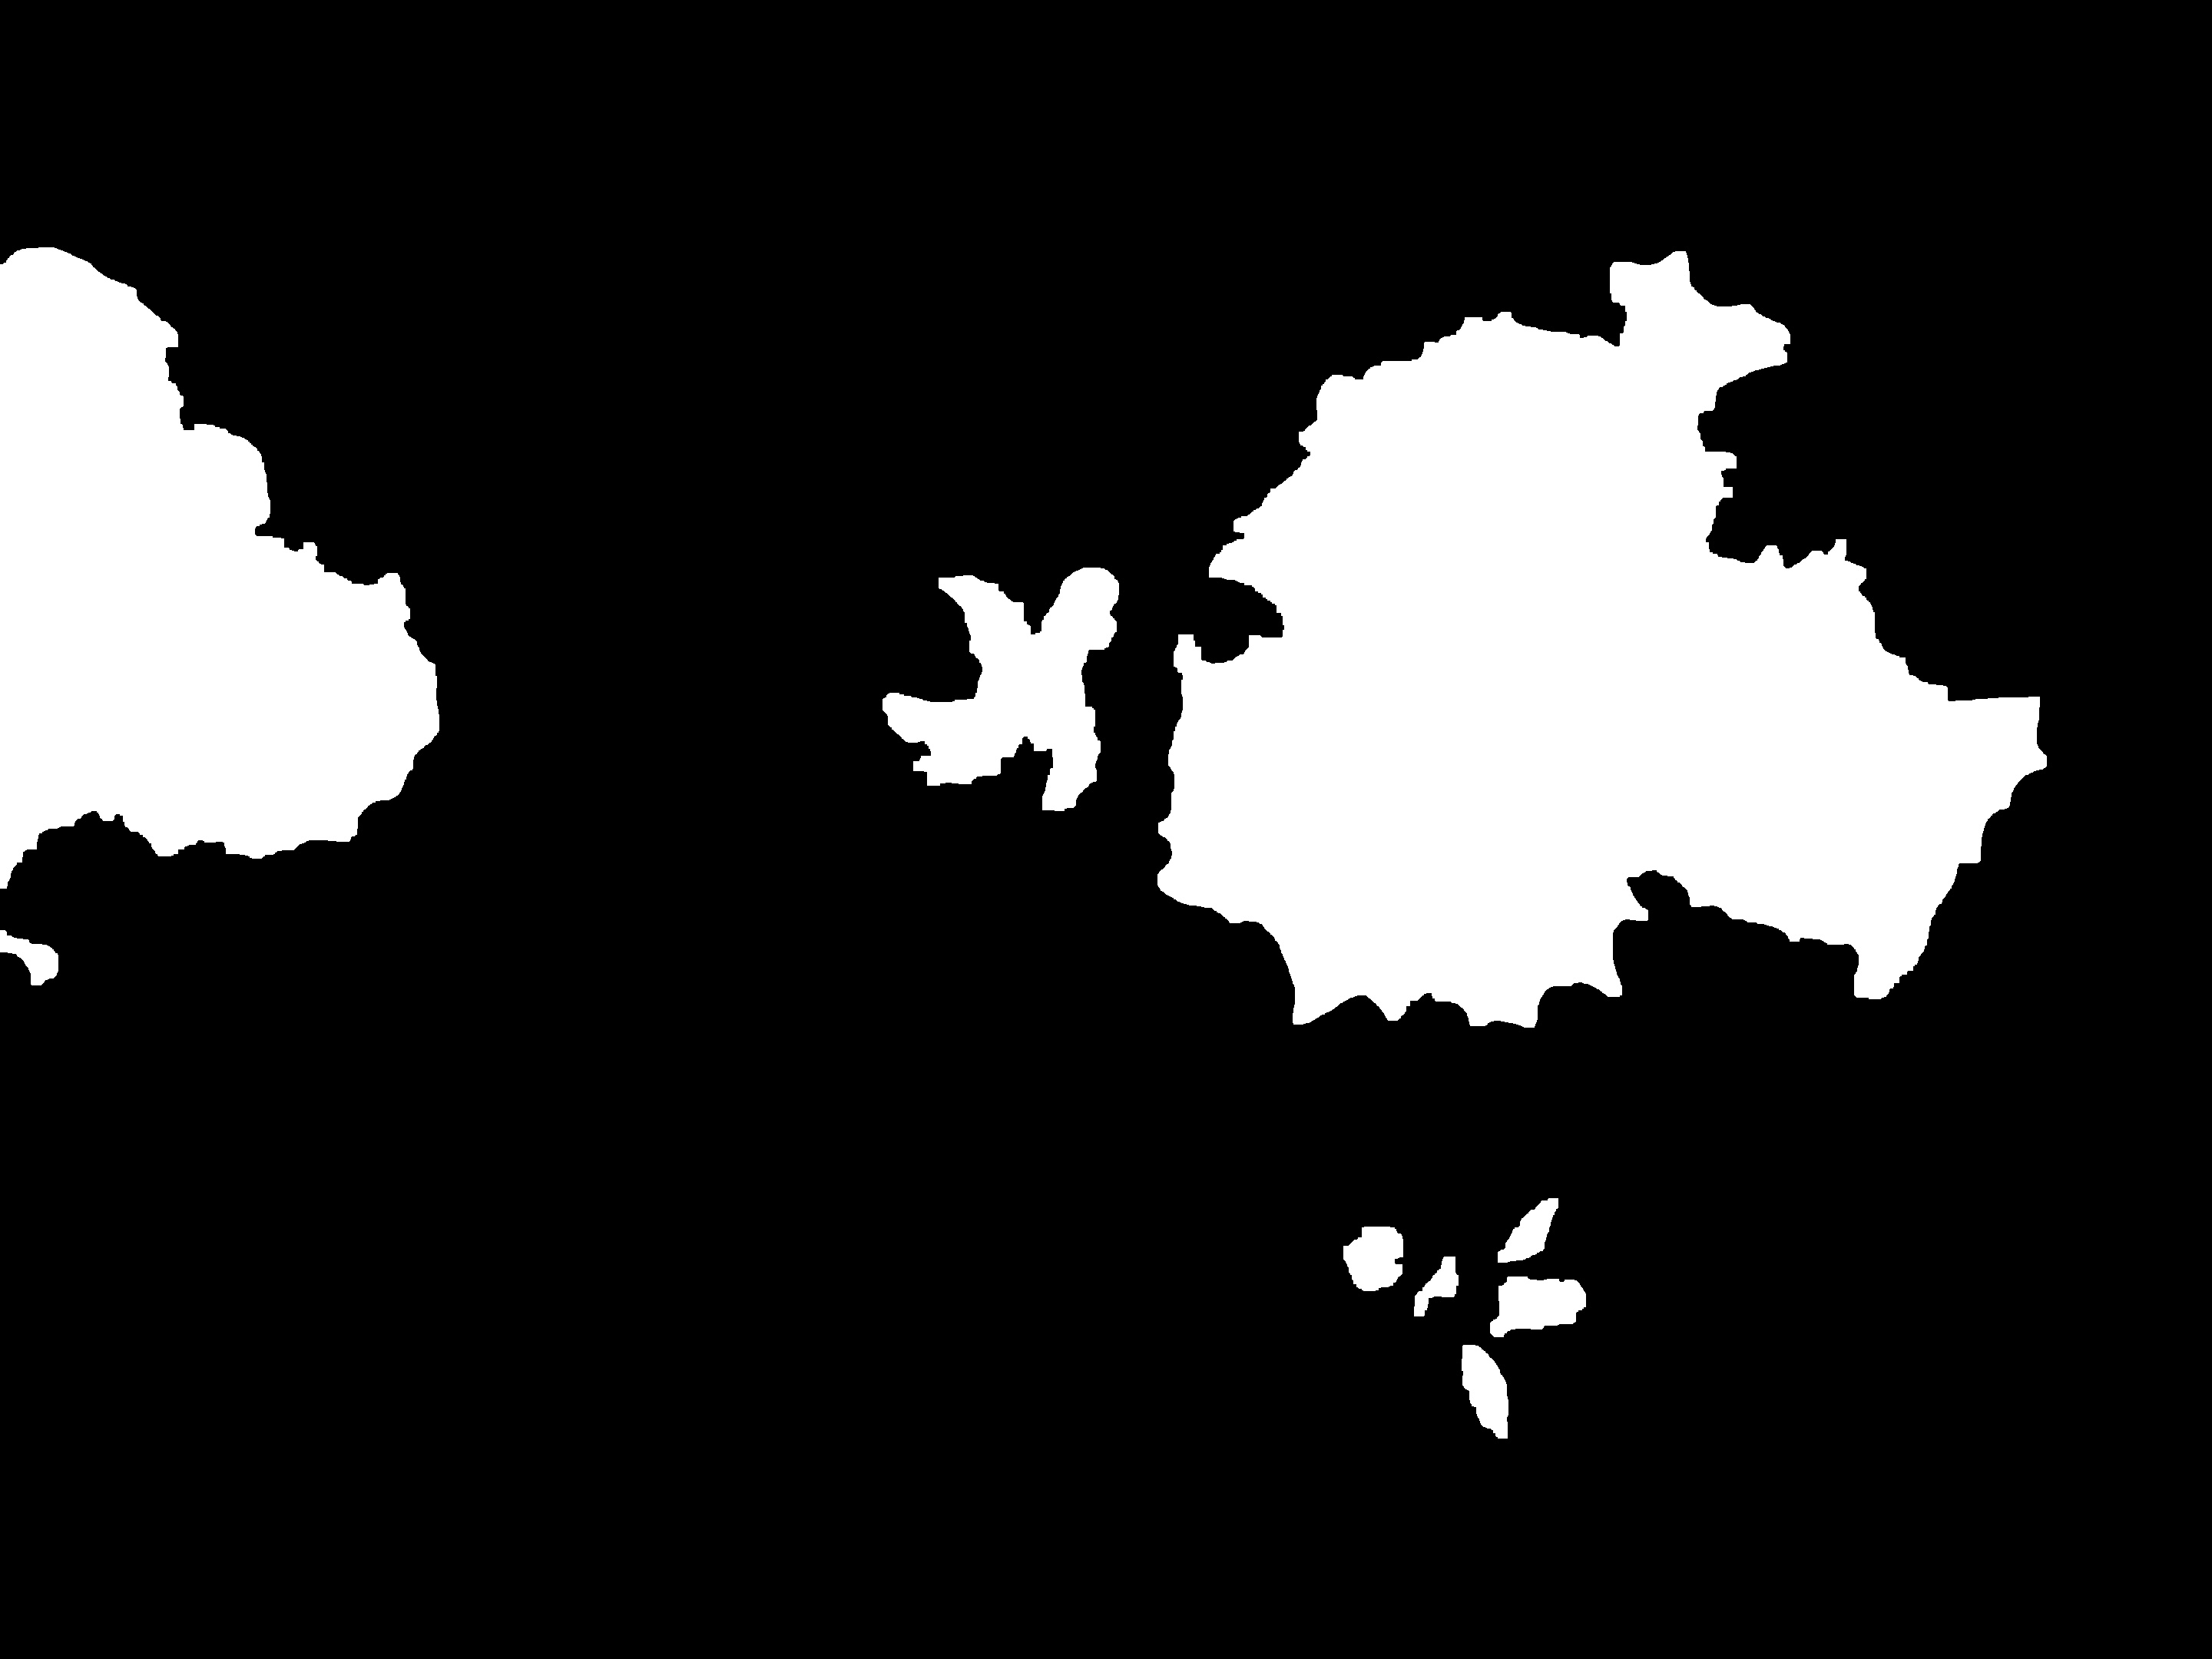
\includegraphics[width=1\linewidth]{figures/original-mask.jpg}
	  \caption{Mask produced with NDI}
	  \label{fig:mask}
	\end{subfigure}
	\begin{subfigure}[h]{.30\textwidth}
	  \centering
	  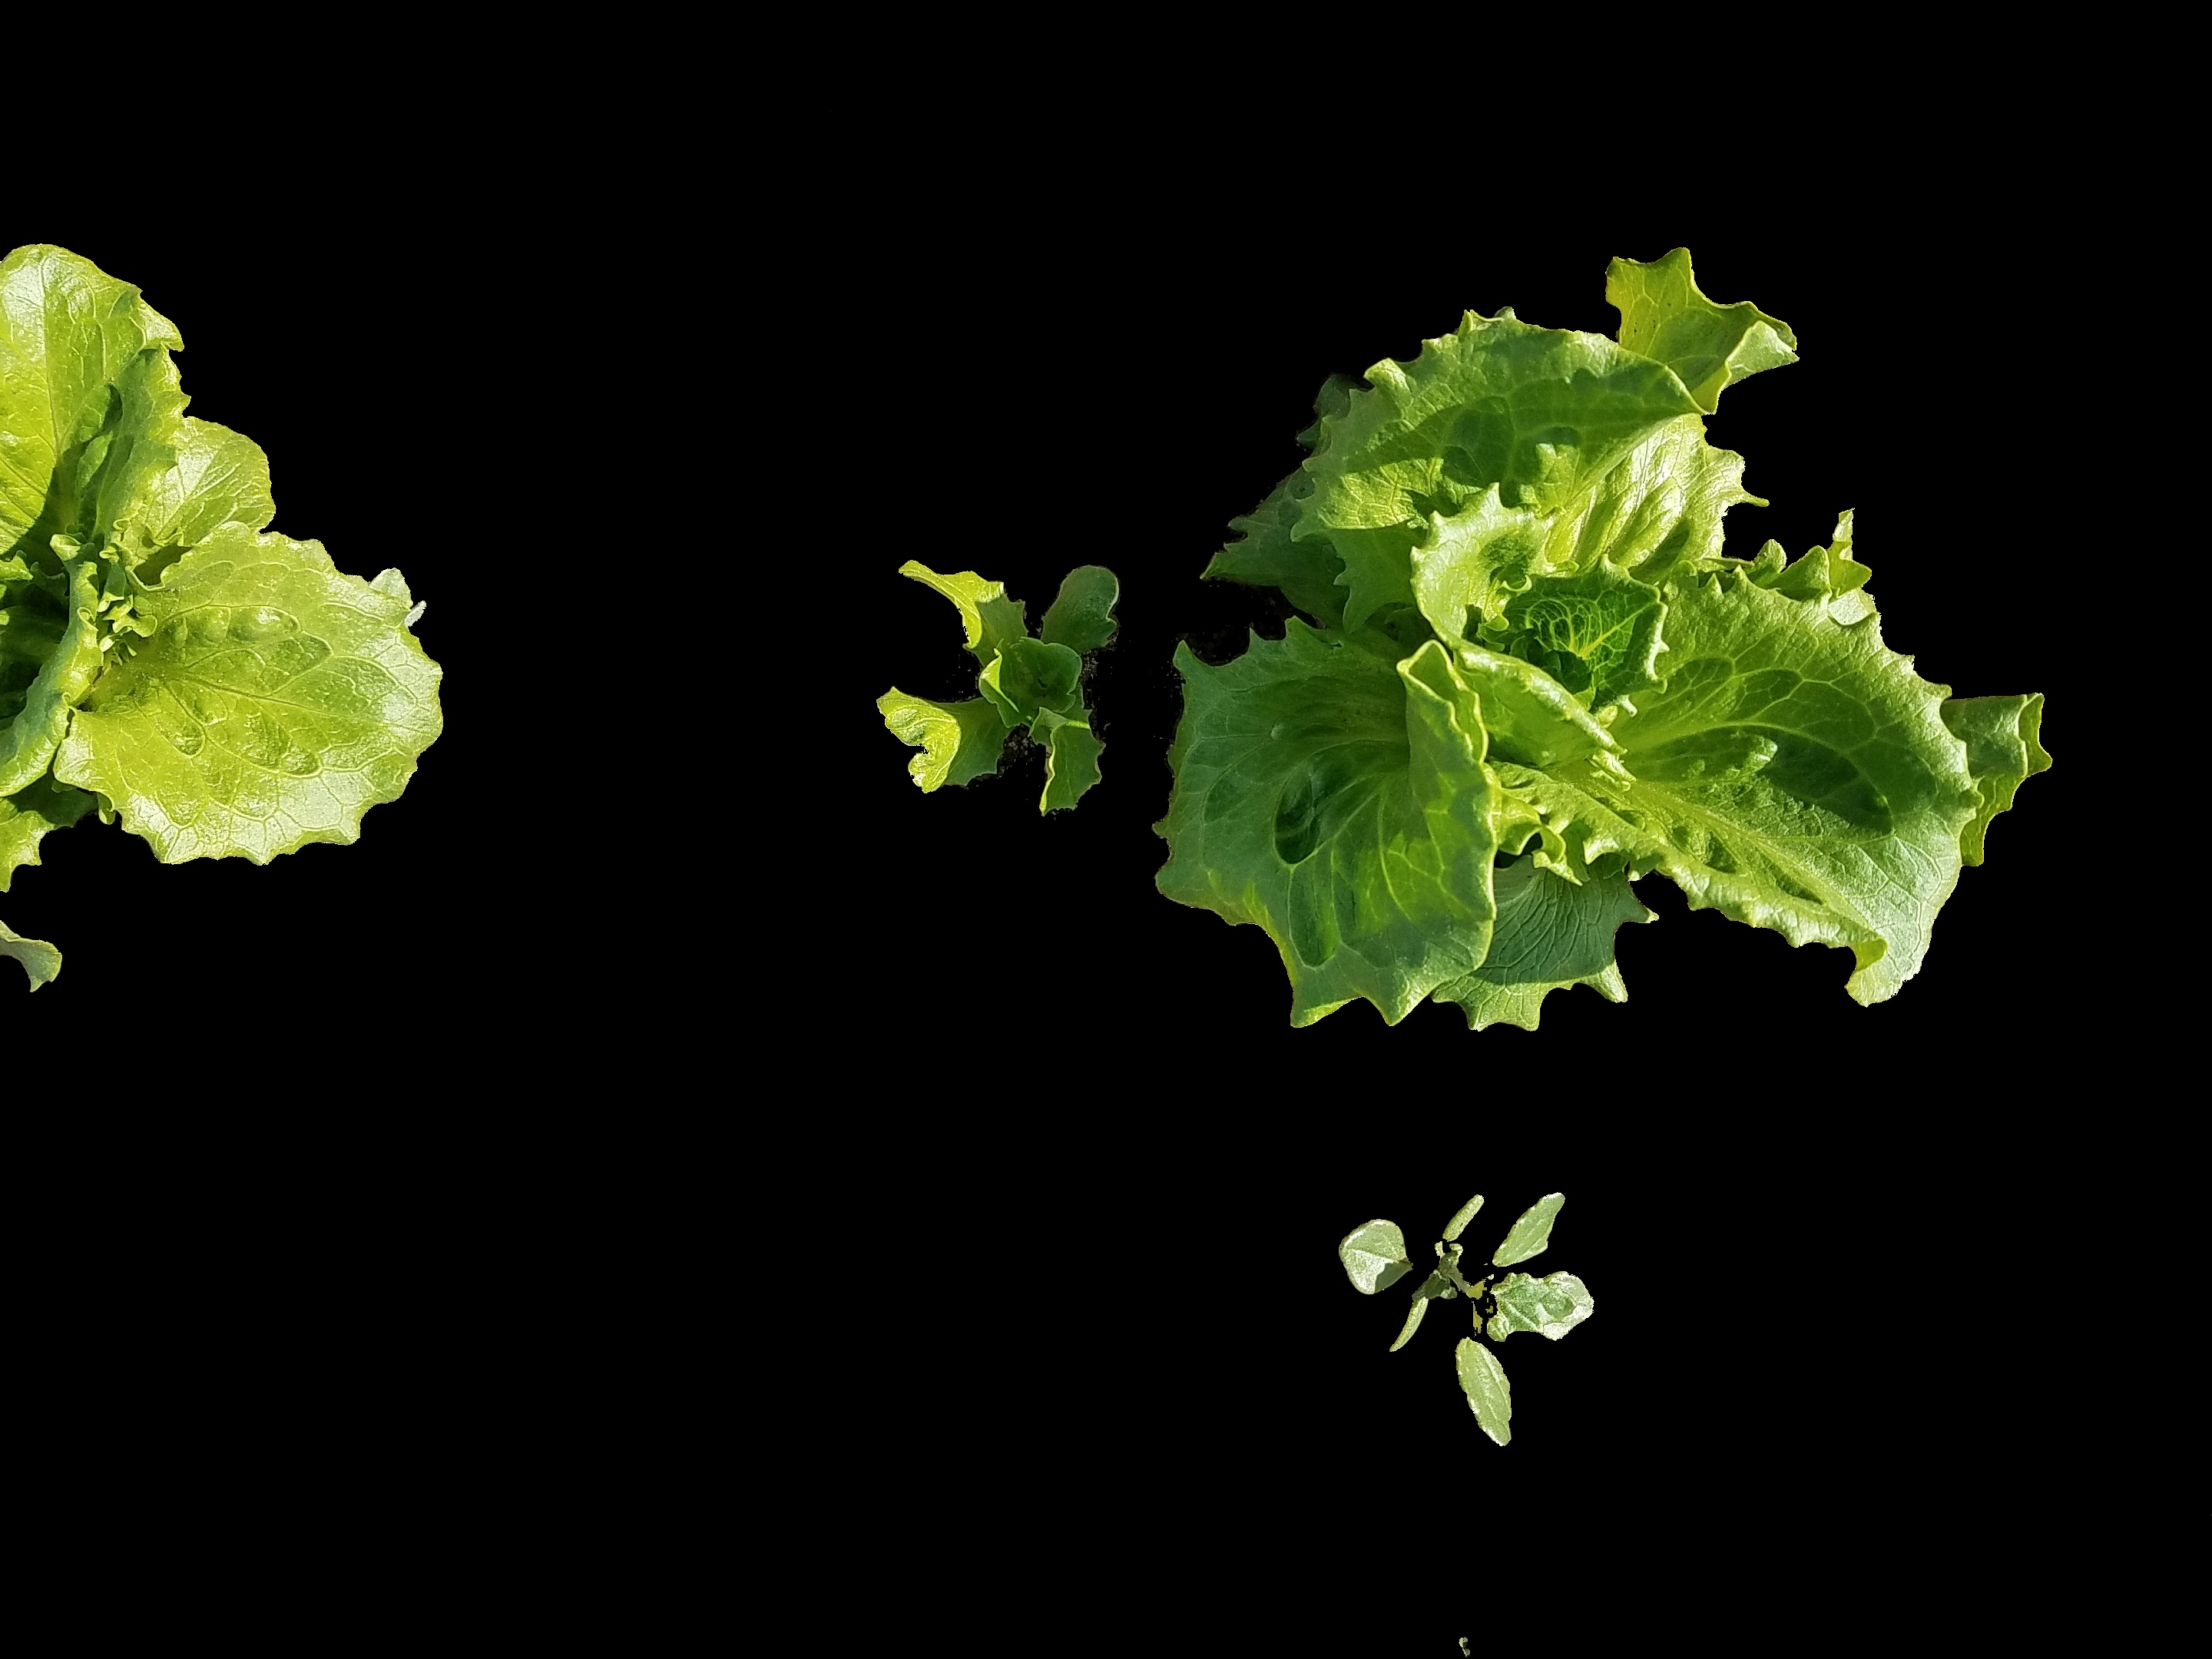
\includegraphics[width=1\linewidth]{figures/original-masked.jpg}
	  \caption{After applying mask}
	  \label{fig:original-masked}
	\end{subfigure}
	\caption[Before and after segmentation]{Before and after segmentation. Note the absence of the stems seen in the weed in the lower portion of~\ref{fig:original-masked} -- this is made a bit more obvious with a close examination of the mask shown in~\ref{fig:mask}. The lack of stems will lead to a single plant being identified as multiple plants, but has no effect on the classification using the features identified as significant.}
	\label{fig:segmentation}
\end{figure}
The segmented image has discarded ground pixels while retaining most of the pixels that will be used, but a close examination reveals that pixels in the stems of the weed are also eliminated, as they are less green than the rest of the plant. This effect is even more pronounced when segmenting images of weed that do not contain green stems as would be seen in the red stems seen in \textit{Portulaca oleracea} (Purslane). While they are not eliminated, pixels in the area of the deep shadows of the vegetation may affect attempts to classify objects based on color attributes. Unfortunately, the band of color featured in the stems (red) is frequently found in the background (soil), so attempts to make the stems appear in the masked image are problematic, as this solution tends to bring allow unwanted ground pixels in the final image that contain hues found within the stems. Likewise, immature vegetation where stems are not sufficiently green will not appear in the final image. Fortunately, both of these cases do not appear to have an appreciable effect on the classification. For the purposes of this paper, images will use the \textit{Normalized Difference Index} (NDI) segmentation approach (see Table~\ref{table:segmentation} for this formula). This process results in image data with only two sets of values: RGB values of zero where there is no vegetation and the original RGB values for pixels containing vegetation. Figure~\ref{fig:ndi-segmentation} illustrates the values used in producing a mask, but here we see a problem introduced.

The creation of an index has produced data that often exaggerates portions of the image with vegetated pixels, but deciding what portions of the data to discard and which to keep can be automated. The manual selection of a threshold can be shown to work relatively well, and can be fine-tuned by examining the results ensure that the number of vegetated pixels are maximized, while the number of non-vegetated pixels are minimized (in other words, we do not want to have significant portions of the ground in the image, but we do want as much of the plant as is possible. An alternative, first proposed by \citeauthor*{Otsu1979-io}  \parencite{Otsu1979-io}, is to select this threshold automatically, or an alternative \textit{Triangle} algorithm used here.

\begin{figure}[h!]
	\centering
	\begin{subfigure}[h]{.48\textwidth}
	  \centering
	  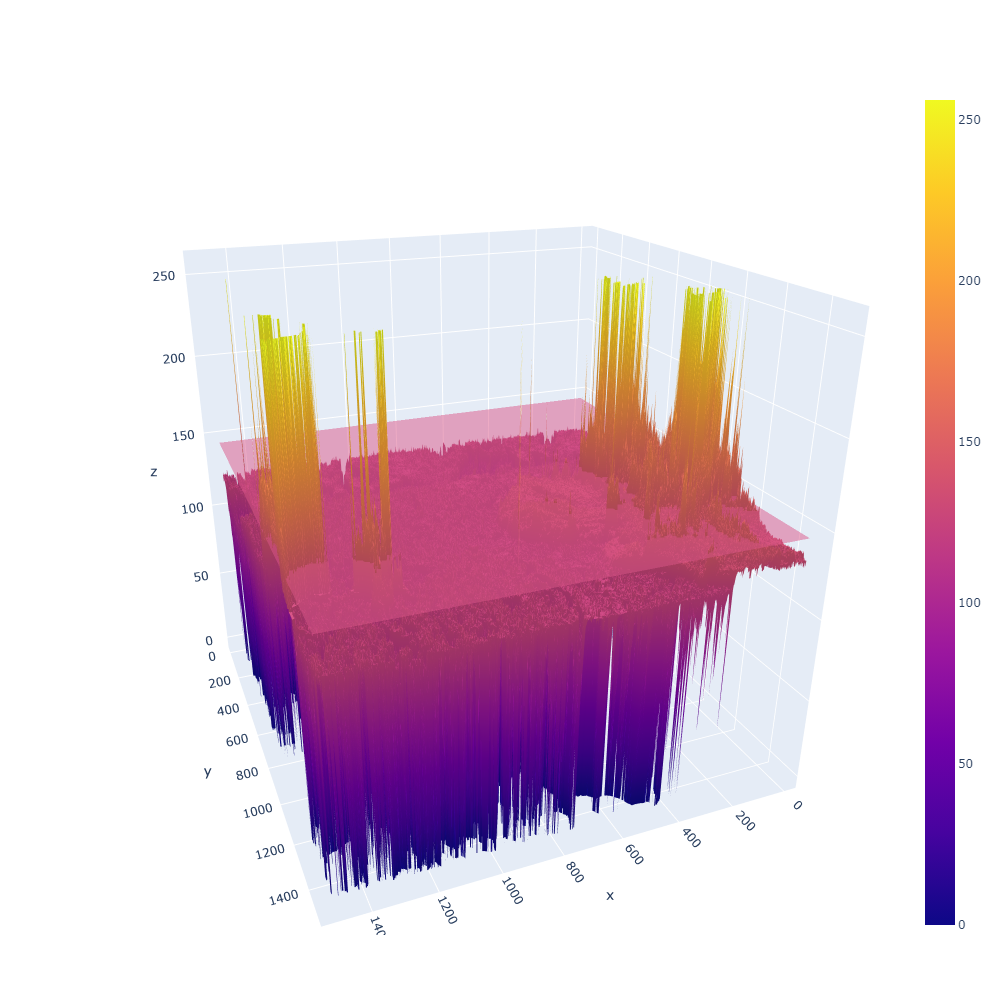
\includegraphics[height=5cm]{./figures/ndi-1-of-2.png}
	  \caption{Image segmented using NDI}
	  \label{fig:ndi-1}
	\end{subfigure}
	\hfill
	\begin{subfigure}[h]{.48\textwidth}
	  \centering
	  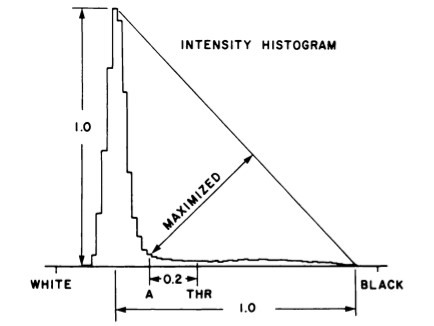
\includegraphics[height=5cm]{./figures/triangle-algorithm}
	  \caption{Triangle method for threshold selection.}
	  \label{fig:ndi-2}
	\end{subfigure}
	\caption[NDI segmentation and threshold selection]{An example of NDI segmentation and threshold selection. A threshold for the production of a mask can be done manually, perhaps by selecting all values below 140 to form the mask that will be applied to the image, illustrated by the semi-opaque plane. While that manual selection may be sufficient to perform the segmentation of an image set acquired under the same ambient conditions, it may lead to the exclusion of portions of the plant in images taken under different conditions. Using the Triangle algorithm \parencite{Brink1996-xy,Zack1977-yl} allows this selection to be made automatically. The point at which the line between the lowest and highest points in the histogram is selected as the threshold, selecting a threshold applicable to each image in a set rather than a global value used for all images in a set.}
	\label{fig:ndi-segmentation}
\end{figure}



\section{Blob Identification}
Segmented images yield images with only vegetated pixels. Single items within those images are often called (somewhat generically) \textit{blobs}, and as that is the term generally used by the OpenCV software libraries used for image processing, that is the term adopted for this document. Blobs are the largest area of contiguous pixels with non-zero values.  The mask produced in the previous section is quite close to being suitable for the purposes of masking out non-vegetated pixels while allowing vegetated pixels of the original image, but requires some further refinement with morphological operations \textit{dilation} and \textit{closing} before it can be used, as the mask produced using only the index tends to hide portions of the vegetation.

\begin{figure}[h!]
	\centering
	\begin{subfigure}[h]{.48\textwidth}
	  \centering
	  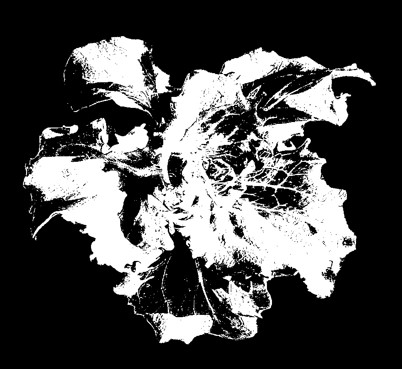
\includegraphics[height=5cm]{./figures/mask-raw.jpg}
	  \caption{Unrefined mask}
	  \label{fig:mask-raw}
	\end{subfigure}
	\hfill
	\begin{subfigure}[h]{.48\textwidth}
	  \centering
	  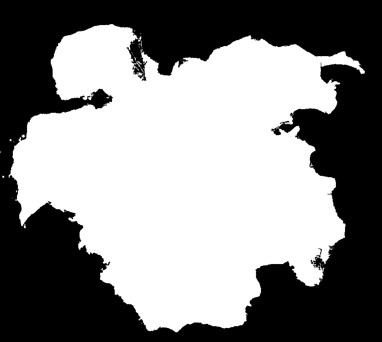
\includegraphics[height=5cm]{./figures/mask-processed.jpg}
	  \caption{Mask refined with pixel dilation and closing}
	  \label{fig:mask-processed}
	\end{subfigure}
	\caption[Mask before and after morphological refinements]{The unprocessed and refined mask. The unrefined mask in Figure~\ref{fig:mask-raw} would not allow for many of the details of the plant to be present in the final image. Note that large portions of some of the leaves are rendered as black, even as the vegetation edges are not. After the pixels are dilated with a 5x5 kernel of all 1s, the mask shown in Figure~\ref{fig:mask-processed} is produced, allowing all pixels within the leaf area to be present in the final image.}
	\label{fig:mask-before-and-after}
\end{figure}


Blobs are identified as an object requiring classification, but not yet classified. Figure~\ref{fig:original-masked} is an example of this concept. This image shows eight blobs that can be classified: three lettuce plants and a single weed plant that appears as five plants in the final image.

\section{Feature Extraction}
Once the vegetation is isolated and blobs identified, various features can be extracted for subsequent use in classification. These features include position-independent characteristics such as shape, hue, and textural characteristics as well as position-dependent features such as where a plant resides relative to the crop-line and size ratios between objects.  

\subsection{Shape Characteristics}
The shape of an object can be globally or locally described by various factors \parencite{Zhang2004-cm}. The problem quickly encountered in using shape in this instance is that a 3D object is projected on to a 2D plane, losing information in the process. The object in the resulting image is, of course, only a partial representation of the object as it exists in the real world. As section \ref{problem-overlap} shows in greater detail, even simple, but common occurrences such as object overlap complicate attempts to exploit shape. The classification examined in this paper will consider only the former, global descriptors that apply to an entire object. Shape parameters used in classification must exhibit three characteristics: scale invariance, rotation invariance, and translation invariance. Rotation invariance is, perhaps, the most relatable of these. While a camera mounted on a UAV or tractor will collect imagery in the same orientation, plants are not so obliging in their growth. Two plants might have leaves that may look extremely similar (and could be said to be of the same shape), but are rotated by 90\si{\degree}. Scale invariance is almost as easy to describe: two leaves have the same shape, but are simply of different size due to differences in the time of emergence. Translation invariance means that the same descriptor is derived without considering the position of the object within the image.  A fourth invariance is a bit more complex: viewpoint. While a camera capturing images as it passes overhead can always -- within a very small variation -- be considered to have the same viewpoint, the same does not hold true for the plants in the image. Two leaves can have the same physical shape, but differences in orientation with respect to the Z-axis (consider the case where the tip of one leaf is closer to the ground) produce significantly different descriptions of their shape. While a perfect shape descriptor would be invariant under all of these, it is typically not realistic to arrive at a shape descriptor that is invariant in all cases.
The shape parameters considered in this analysis are expressions describing the perimeter of the plant. The shape formulae used to extract the various shape features are given in Table~\ref{tab:shape-formulae}, but some concepts and formulae warrant further explanation.

\subsubsection{Bounding Box and Convex Hull}
An object can be said to have rectangular box of minimum size that completely encloses the object, commonly termed the \textit{bounding box}. The box placed around the object without regard for orientation -- that is, the placement makes no attempt to align the edges of the box with the edges of the image, so it may appear tilted at normal viewing angles. The \textit{convex hull}, likewise, is a convex shape with straight lines and of minimum size that completely encloses the object.   
\begin{figure}[h!]
	\centering
	\begin{subfigure}[h]{.48\textwidth}
	  \centering
	  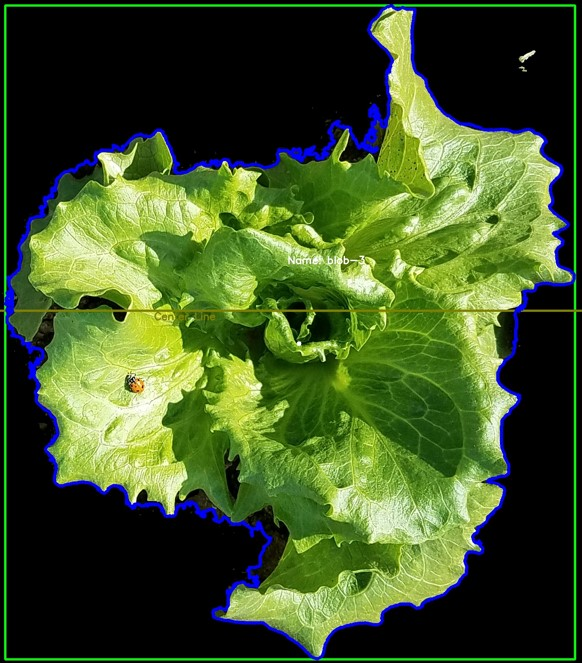
\includegraphics[height=5cm]{./figures/shape-bounding-box.jpg}
	  \caption{A bounding box}
	  \label{fig:bounding-pox}
	\end{subfigure}
	\hfill
	\begin{subfigure}[h]{.48\textwidth}
	  \centering
	  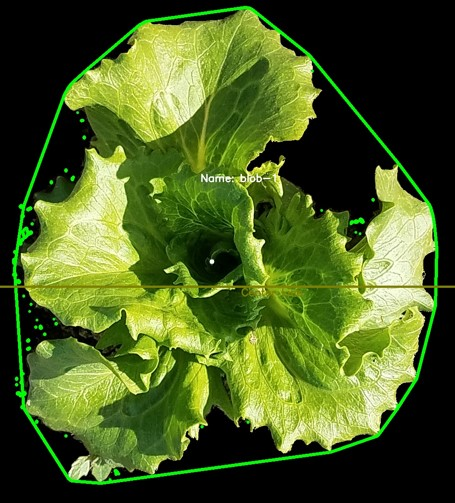
\includegraphics[height=5cm]{./figures/shape-convex-hull.jpg}
	  \caption{A convex hull}
	  \label{fig:convex-hull}
	\end{subfigure}
	\caption[Bounding box and convex hull]{A bounding box and a convex hull (both noted in green) surround an object, but a convex hull is a shape with the minimum size that can contain the object. A bounding box is the minimum sized rectangle that can contain the object.}
	\label{fig:bounding-and-hull}
\end{figure}
The convex hull is a simple polygon whose vertices are a subset of the points found in the edge of the original shape. A widely used algorithm for determining the convex hull, \textit{Graham's Scan} is fairly efficient, $\mathcal{O}(n\log n)$, as \citeauthor{Klette2004-qz} show in this excerpt (altered for clarity with assistance from lecture notes from \citeauthor{Prosser1998-mi}). \parencite{Klette2004-qz}
\begin{quote}
\begin{enumerate}
	\item{Find the bottom-most point by comparing \textit{y} coordinate of all points. If there are two points with the same \textit{y} value, then the point with smaller \textit{x} coordinate value is considered. Let the bottom-most point be $P0$. Put $P0$ at first position in output hull.}
	\item{Sort the remaining points $p_i$ of $S$ in order of increasing angles $\eta_i$; if the angle is the same for more than one point, keep only the point furthest from $p$. Let the resulting sorted sequence of points be $q_i,..., q_m$.}
	\item{Initialize $C(S)$ by the edge between $p$ and $q_1$.}
	\item{Scan through the sorted sequence. At each left turn, add a new edge to $C(S)$; skip the point if there is no turn (a collinear situation); backtrack at each right turn.}
\end{enumerate}
\end{quote}
The most salient problem with the convex hull, however, is one that will have an adverse affect on all shape descriptors: distortions introduced by the resolution of the same object at different altitudes. That is, the edges are described by fewer pixels as the distance between the camera and plant increases, resulting in increased pixelation. While this can be minimized to some extent by blurring the image prior to performing the hull calculations, the hull is still distorted by this lower resolution.

\subsubsection{Area \& Size Ratio}
The area of the plant in the segmented image is simply the number of pixels with non-zero values. The relative area of two plants can then be compared to predict membership in a class. For instance, if a plant is $\frac{1}{3}$ the size of the largest plant in the image it is more likely than not a weed. This ratio is highly dependent on the development phase of the crop, as the reverse could be true for crop just emerging compared to much larger weeds. For the classification purposes presented here, the larger item is presumed to be crop.

\subsubsection{Length/Width Ratio}
\label{sec:width-length-ratio}
The ratio of width to length is not -- as the name might imply -- a simple ratio of two measurements, but is expressed as:
\begin{equation}
S = 
	\begin{bmatrix}
	Var(X) & Cov(XY) \\[0.3em]
	Cov(XY) & Var(Y) \\[0.3em]
	\end{bmatrix},
\lambda = \frac {eig_{1}(S)} {eig_{2}(S)}
\end{equation}
Where $eig_{1}(S)$ and $eig_{2}(S)$ are the maximum eigenvalues of the matrix $S$, with $\lambda$ representing the ratio. (\cite{Lin2017-xq}) The X and Y positions refer to an object's perimeter -- the boundary between an object's edge and the background.

\subsubsection{Boundary Descriptors}
Once again focusing on the edge of an object, a global descriptor of the shape is the \textit{k-curvature} of the edges, but arriving at this global descriptor involves a few preliminary steps. Changes in the $(x,y)$ position of edge pixels can be described by a \textit{chain code}. A chain code representation of a boundary describes unit length changes in the $(x,y)$ positions of the boundary,  where changes in the position are noted by their position in a matrix:

 \begin{figure}[h!]
	\centering
	\begin{subfigure}[h]{.4\textwidth}
	  \centering
	  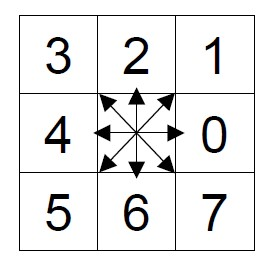
\includegraphics[height=3cm]{./figures/chain-code-matrix.jpg}
	  \caption{Chain code matrix}
	  \label{fig:chain-code-matrix}
	\end{subfigure}
	%\hfill
	\begin{subfigure}[h]{.4\textwidth}
	  \centering
	  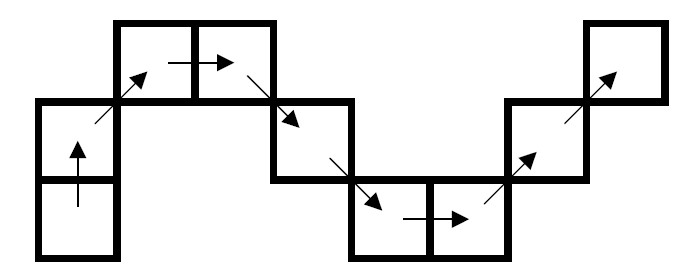
\includegraphics[height=3cm]{./figures/chain-code-cells.jpg}
	  \caption{Example edge}
	  \label{fig:chain-example}
	\end{subfigure}
%	\hfill
%		\begin{subfigure}[h]{.25\textwidth}
%	  \centering
%	  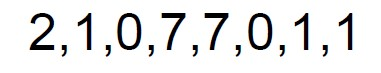
\includegraphics[height=2cm]{./figures/chain-code-result.jpg}
%	  \caption{Result}
%	  \label{fig:chain-result}
%	\end{subfigure}
	\caption[Boundary chain codes]{Chain codes of the transitions of an object's edge -- as seen in successive pairs of coordinates -- are described by positions within an 8 position matrix, with each position noting the change in the $(X, Y)$ coordinate (steps of length 1 along the $x,y$ axis lines and of length $\sqrt{2}$ for diagonal movements). In this example the edge has a chain code of 2,1,0,7,7,0,1,1. While this example shows an open curve with a distinct beginning and ending, the boundary of a plant is a closed curve with no distinct end or beginning. A 4 direction matrix is is also used, as is a general $N$-directional chain $(N > 8\ and\ N =2^k)$, although those variants are not addressed in this document. The 8 position matrix is, perhaps, the most relatable, as changes in adjacent boundary pixels always take one of the 8 possibilities present in the matrix. The matrix shown in \ref{fig:chain-code-matrix} is a $3x3$ matrix, but the middle position (implying no change) is not possible -- this is simply an illustration.}
	\label{fig:chain-codes}
\end{figure}

The \textit{$\kappa$-slope} of a given boundary point $(X_i, Y_i)$ is estimated from the slope of the line joining positions $(X_{i-k/2}, Y_{i-k/2})$ and $(X_{i+k/2}, Y_{i+k/2})$ with this equation:
\begin{equation}
\tan^{-1}\left(\frac{Y_{i+k/2} - Y_{i-k/2}}{X_{i+k/2} - X_{i-k/2}}\right)
\end{equation}
 
 The \textit{$\kappa$-curvature} of the boundary at location $(X_i,Y_i)$ can be estimated by this equation:
 \begin{equation}
 \tan^{-1}\left(\frac{Y_{i+k} - Y_{i}}{X_{i+k} - X_{i}}\right) - \tan^{-1}\left(\frac{Y_{i} - Y_{i-k}}{X_{i} - X_{i-k} }\right)
 \end{equation}
 The goal of this metric is to assess the concavity or convexity of points along the perimeter. Consider the weed in this image with the computed $\kappa$-curvature:
 
  \begin{figure}[h!]
	\centering
	\begin{subfigure}[h]{.4\textwidth}
	  \centering
	  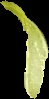
\includegraphics[height=4cm]{./figures/for-curvature-blob-1.jpg}
	  \caption{Weed}
	  \label{fig:curvature-weed}
	\end{subfigure}
	%\hfill
	\begin{subfigure}[h]{.4\textwidth}
	  \centering
	  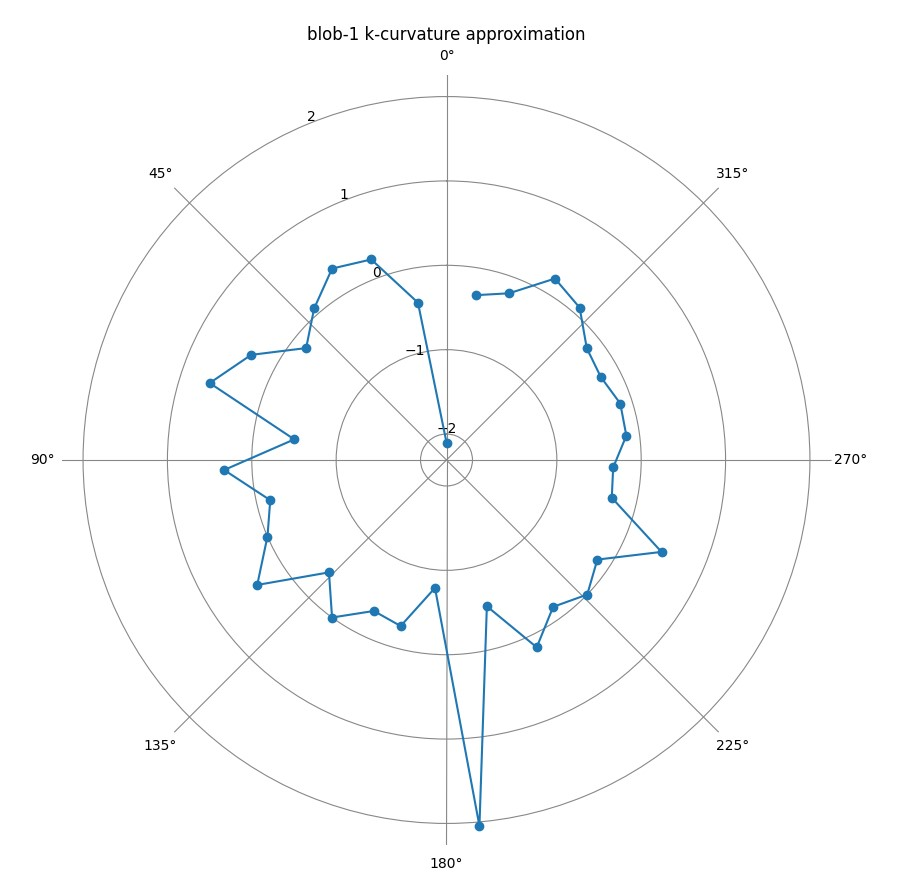
\includegraphics[height=4cm]{./figures/curvature-blob-1.jpg}
	  \caption{$\kappa$-curvature}
	  \label{fig:curvature-plot}
	\end{subfigure}
	\caption[Example of $\kappa$-curvature]{The $\kappa$-curvature of various points around the perimeter of the weed are illustrated here. Positive values are indicative of convex shapes. Likewise, negative values indicate concave shapes.  While it is tempting to relate the values shown in the graph to the image displayed (as the figure invites the user to do), exact correlation is not advised, as the points sampled may not match the finer details that can be seen in the leaf. This example uses a relatively coarse sampling. However, the image does show a pronounced curve at the lower edge that can be seen in the curvature plot.}
	\label{fig:curvature}
\end{figure}
This leads to a global descriptor used in classification: \textit{bending energy}. Bending energy is typically described as the energy required to bend a rod to the shape under consideration, and is expressed as the sum of squares of the $\kappa$-curvature over the boundary length $L$.
\begin{equation}
\frac{1}{L} \sum_{p=1}^{L}\kappa(p)^2
\end{equation}
While there will be no bending of rods required for classification, this global metric can be used to express the overall shape of the perimeter, exploiting the fact that weeds in a crop and the crop itself exhibit different shapes.

The aspects of the \textit{radial distance} can also be used to describe the shape. \citeauthor{Kilday1993-aq}, in a study of classification of lesions in mammogram images, describe techniques to exploit the radial distance of a shape \parencite{Kilday1993-aq}. Before stepping through those techniques, it may prove useful to step back a bit and look at radial distances of an object.
\begin{figure}[H]
	\centering
	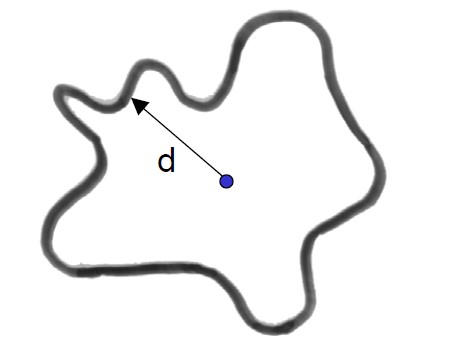
\includegraphics[width=.25\linewidth]{./figures/radial-distance.jpg}
	\caption[Radial distance from object centroid]{The radial distance from object centroid is noted by \textit{d} in this figure. Scale invariance is achieved by expressing functions of the normalized distance (using the maximum radial distance of the object)}
	\label{fig:radial-distance}	
\end{figure}
As Figure \ref{fig:radial-distance} shows, the radial distance referred to is the distance from an object's centroid (geometric center) to its perimeter. To make this distance scale invariant, the normalized distance to the maximal distance is used. Using the normalized radial distance, the mean and standard deviation is given by these equations for the $i^{th}$ blob:
\begin{equation}%\labeleqn{Radial distance mean and standard deviation}
\bar{x}_i = \frac{1}{N}\sum_{k=1}^{N}r_k \qquad
\sigma_i = \sqrt{\frac{1}{N}\sum_{k=1}^{N}({r_k} - \bar{x}_i)^2}
\end{equation}
By themselves these metrics may not be particularly useful in predicting class membership, however these provide useful information for metrics that may be. The number of times the normalized radial distance crosses the mean, for instance, provides an estimate of the roughness of a perimeter.


% Begin table of shape equations
\begin{longtable}{x{\dimexpr.15\columnwidth-2\tabcolsep}
                  x{\dimexpr.425\columnwidth-2\tabcolsep}
                  x{\dimexpr.425\columnwidth-2\tabcolsep}}
%\begin{hyphenrules}{nohyphenation}
    \caption{Shape Features}\label{tab:shape-formulae}  \\
\toprule
{\textbf{Feature}} & {\textbf{Formula}} & {\textbf{Comment}}
\tabularnewline
\midrule
    \endfirsthead
%%%%
    \caption{Shape Features (cont.)}\label{tab:shape-formulae}  \\
\toprule
{\textbf{Feature}} & {\textbf{Formula}} & {\textbf{Comment}}
\tabularnewline
\midrule
    \endhead
%%%%
\midrule[\heavyrulewidth]
\multicolumn{3}{r}{\footnotesize\itshape
                   Continued on the next page}
    \endfoot
%%%%
\bottomrule
    \endlastfoot
%%%%
		Perimeter
		& \begin{minipage}[t]{0.3\textwidth}
			$\sum_{i=1} ^{N-1}\left|X_1 - X_{i+1}\right| $
		   \end{minipage}     
		& Count of pixels forming the boundary of an object
\tabularnewline\addlinespace

		Major/Minor Axis     
		& $\sqrt{(x_2 - x_1)^2 + (y_2 - y_1)^2} $                    
		& Major axis is the longest line that can be drawn through the object. Minor axis is the longest line that can be drawn through the object such that the line remains perpindicular to the major axis.
\tabularnewline\addlinespace

		Compactness      
		& \begin{minipage}[t]{0.3\textwidth}
			$\frac{4\pi * area}{(perimeter)^2}$ 
		   \end{minipage}
		& Ratio of an object's area to the area of a circle having the same perimeter 
\tabularnewline\addlinespace

		Elongation      
		& $\frac{width_{bounding}}{length_{bounding}}$ 
		& Ratio of the width of the object's bounding box to its width
\tabularnewline\addlinespace

		Eccentricity      
		& $\frac{length_{minor}}{length_{major}}$
		& Ratio of the minor to major axis
\tabularnewline\addlinespace

		Convexity   
		& $\frac{convex~perimeter}{perimeter}$ 
		& Ratio of the convex perimeter to the perimeter.
\tabularnewline\addlinespace

		Solidity    
		& $\frac{area}{convex~area}$ 
		&  Ratio of an object's area to its convex area. 
\tabularnewline\addlinespace

		Circularity    
		& $\frac{4\pi * area}{convex~perimeter}$ 
		& Ratio of an object's area to its convex perimeter. 
\tabularnewline\addlinespace


		Shape Index    
		& $\alpha = \frac {e} {4 \sqrt{A}}$ 
		&  Relationship between an object's perimeter and its area
\tabularnewline\addlinespace

		Width/Length Ratio
		& \begin{minipage}[h]{0.10\textwidth}
			\begin{eqnarray*}
				S = 
				\begin{bmatrix}
					Var(X) & Cov(XY) \\[0.10em]
					Cov(XY) & Var(Y) \\[0.10em]
				\end{bmatrix}
			\lambda = \frac {eig_{1}(S)} {eig_{2}(S)}
			\end{eqnarray*}
		  \end{minipage}
		& See section~\ref{sec:width-length-ratio}
\tabularnewline\addlinespace

		Bending Energy    
		& $\frac{1}{L} \sum_{p=1}^{L}\kappa(p)^2$ 
		&  The energy required to bend a rod to the perimeter shape
\tabularnewline\addlinespace

\label{table:shape-formulae}
\end{longtable}
}

% End table of shape equations

%
% C O L O R
%
\subsection{Color}
Color presentations of an image are ubiquitous, and while the Red-Blue-Green (RGB) color space is widely familiar, an image can be represented in other color spaces. RGB representation is nothing more than three channels, each of which note (respectively) the levels of Red, Greed, and Blue in the image.  Examining each of these channels in isolation usually results in an odd -- but fairly realistic -- view of an object. These other color spaces do not alter the image itself, just the representation.  Choosing to represent the amounts of red, green, and blue in an image is just as arbitrary as other mechanisms, however closely aligned it is with human color perception. Classification will use both components of those representations (i.e., the mean of an object's \textit{hue} in the HSI space) as well as the data contained within those components being used in other techniques (GLCM, for instance). While viewing the vegetation in one of the components can be fairly seen as not accurately representing the same experience one would have in viewing the object in daylight or other presentations, these components often have information relevant to the task at hand. This section presents a brief overview of the color spaces used in classification.

\subsubsection{Hue-Centric colorspaces: HSI \& HSV}
The terms {\it color} and {\it hue} are often used interchangeably, and while this is mostly true, hue refers to the dominant color family. In this case, the image is converted to the Hue, Saturation, and Intensity {\it HSV} colorspace and the mean value for the hue of a blob's pixels is taken. The saturation of a color expressed by a component of the Hue, Saturation, and Intensity ({\it HSI}) colorspace and the mean value for the saturation of a blob's pixels is taken. (\cite{Forsyth2012-hy})

The Hue, Saturation, and Intensity (HSI) and the Hue, Saturation, and Value (HSV) color spaces are cylindrical-coordinate representations of the RGB color model.  These models, first developed in the 1970s, rearrange the RGB cube representation to be more perceptually relevant. Both models are closely related in that they share an common expression of hue and saturation. While it is a bit simplistic to state, and as the similarities in the name imply, the values for \textit{hue} and \textit{saturation} are identical for these two colorspaces, leaving focus on the \textit{intensity} and \textit{value} components as the unique values that will be analyzed. \parencite[p.~84]{Forsyth2012-hy} Somewhat confusingly, HSV is sometimes referred to as HSB (or Hue, Saturation, and Brightness); likewise, HSI is  is sometimes referred to as HSL (Hue, Saturation, and Lightness), but the two are identical for the most part. In this cylindrical representation, hue is expressed as the angular dimension, red (at 0\si{\degree}), passing through green (at 120\si{\degree}) and blue (at 240\si{\degree}) In each representation, the vertical axis comprises the neutral, achromatic, or gray colors ranging, from top to bottom, white at lightness 1 (value 1) to black at lightness 0 (value 0).

\begin{figure}[H]
	\centering
	\begin{subfigure}[h]{.45\textwidth}
		\centering
		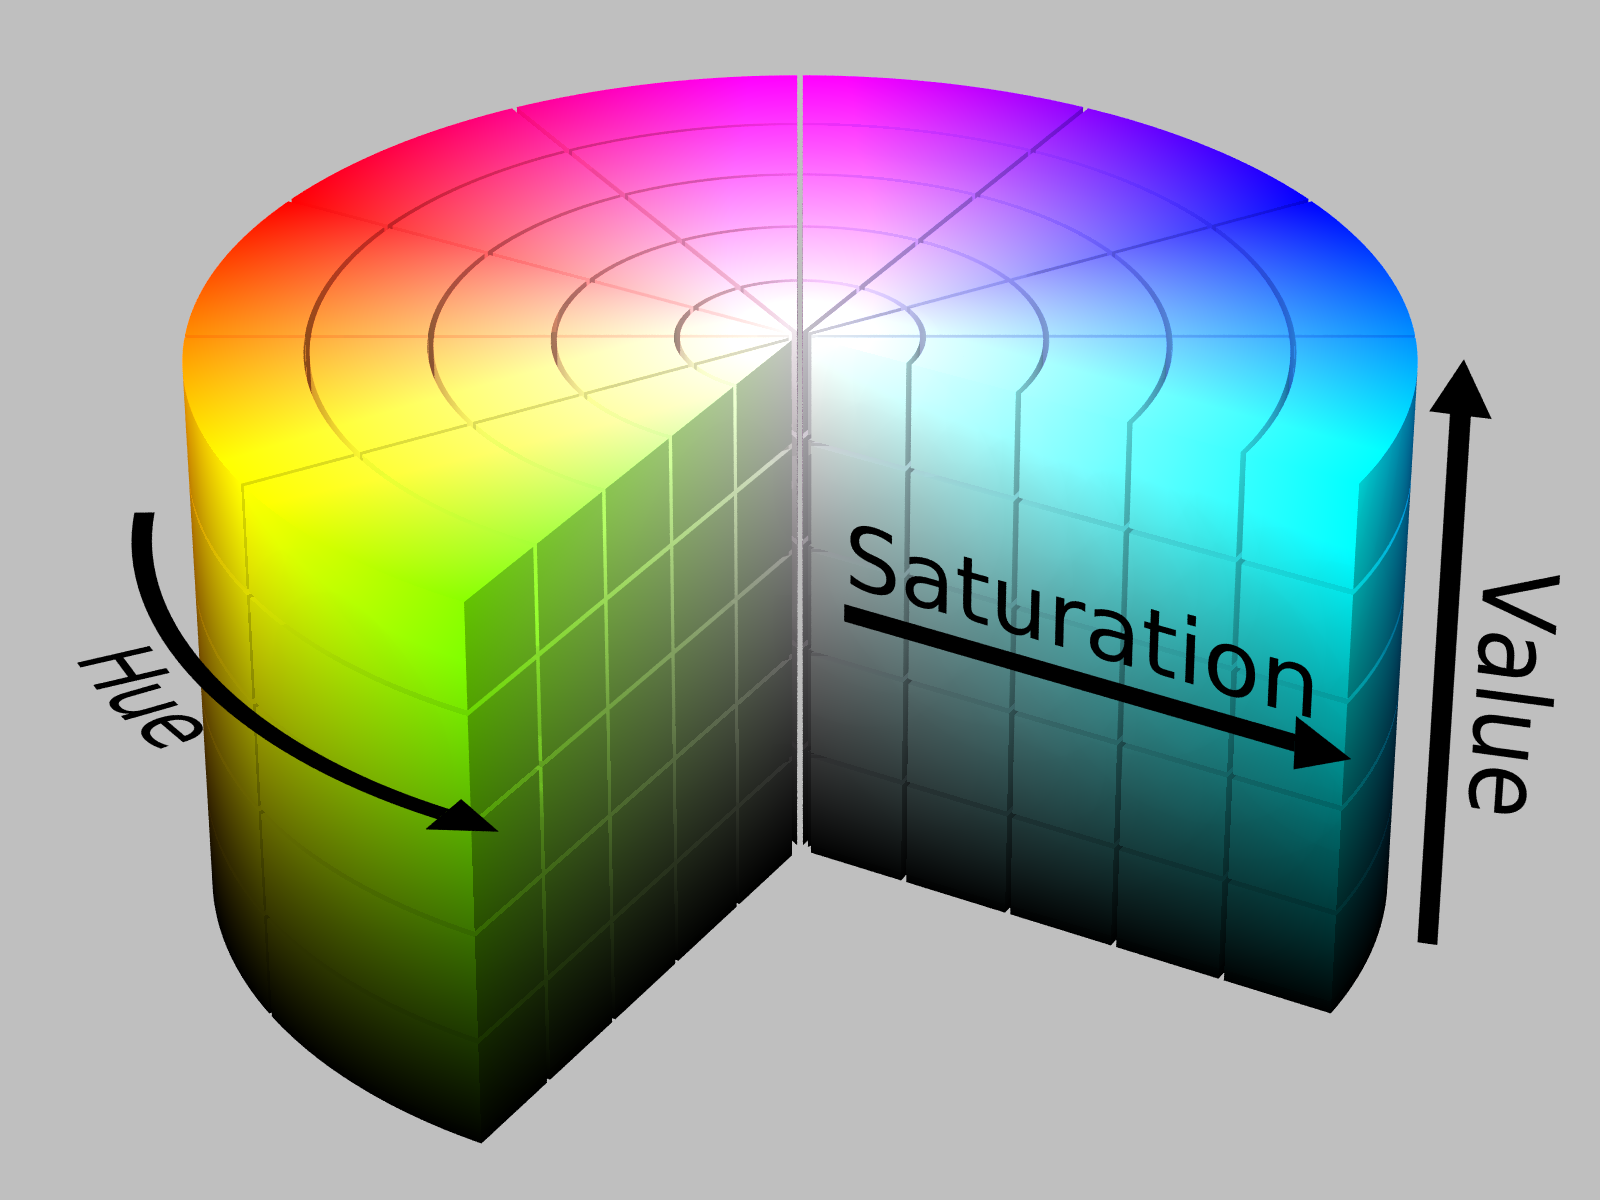
\includegraphics[width=6cm]{./figures/HSV_color_solid_cylinder_saturation_gray.png}
		\caption{HSV/HSB Cylinder}
		\label{fig:hsv}
	\end{subfigure}
	\hfill
	\begin{subfigure}[h]{.45\textwidth}
		\centering
		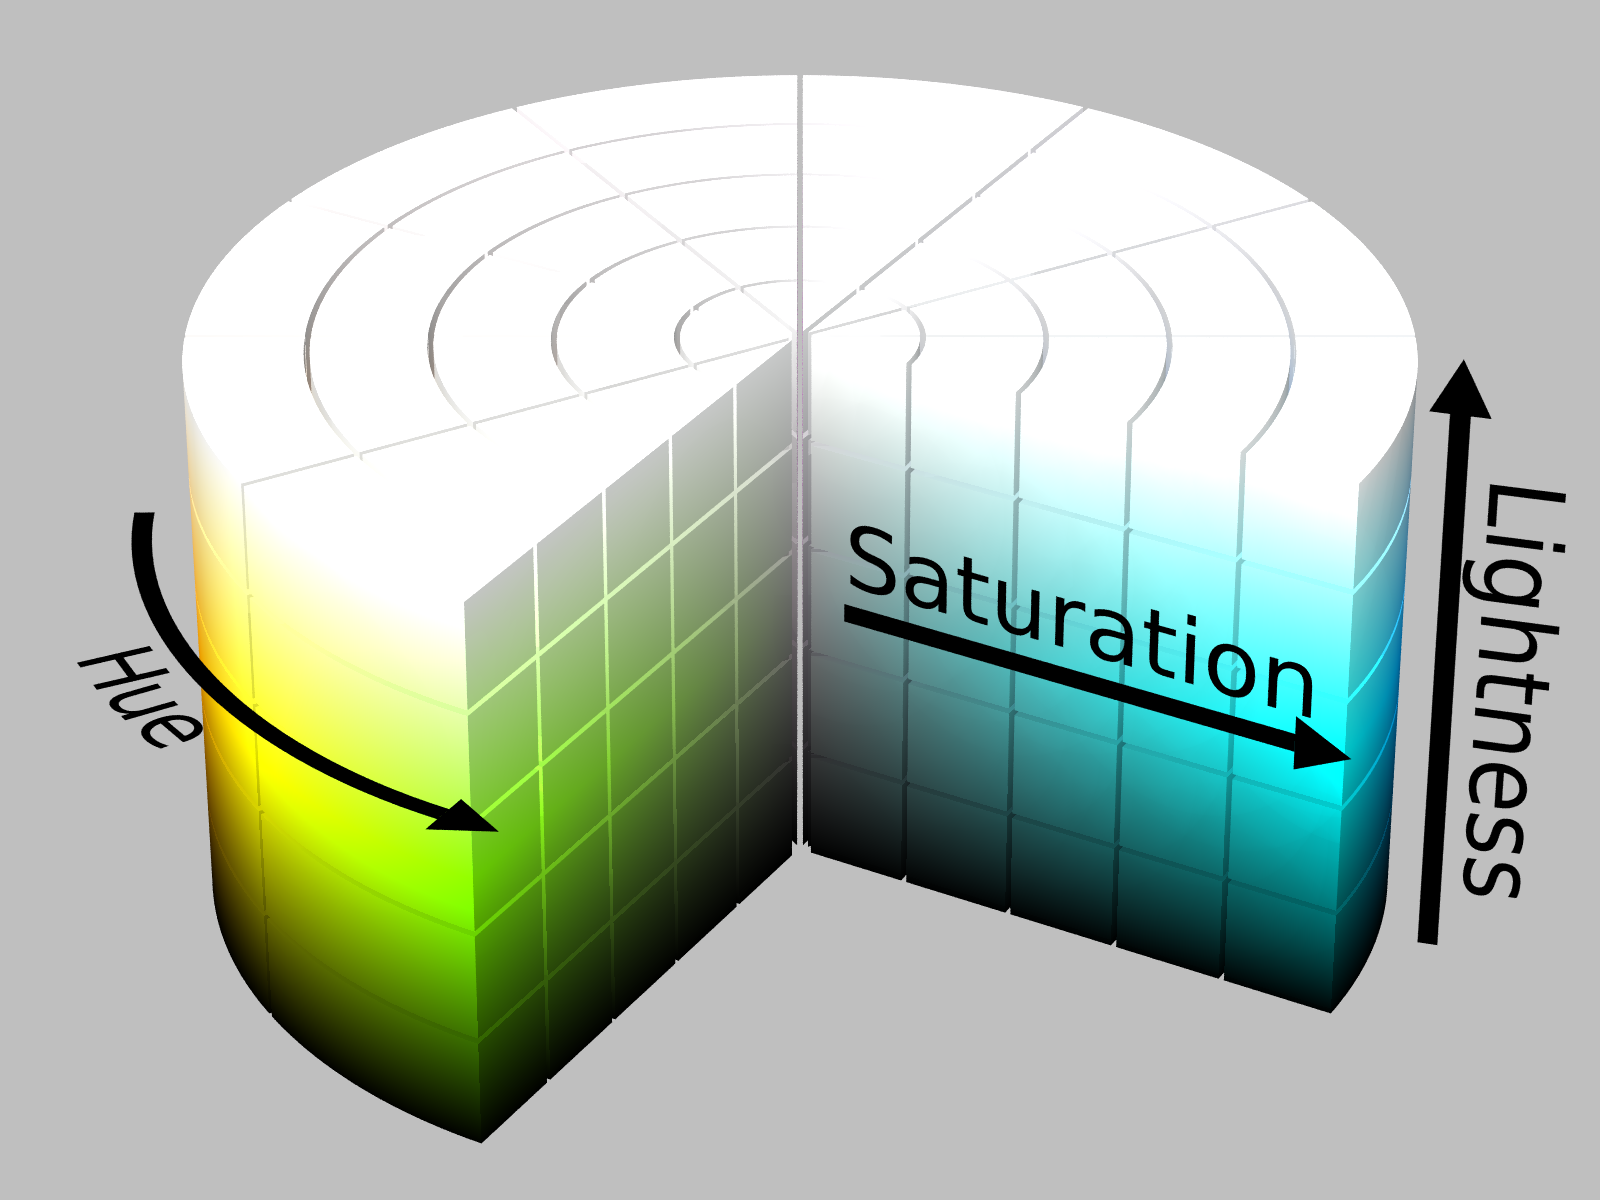
\includegraphics[width=6cm]{./figures/HSL_color_solid_cylinder_saturation_gray.png}
		\caption{HSL/HSI Cylinder}
		\label{fig:hsl}
	\end{subfigure}
	\caption[HSL and HSV color representations]{HSL and HSV color representations. (Creative Commons)}
	\label{fig:overlap}
\end{figure}

\subsubsection{YIQ}
The YIQ model of color was used by the (analog) NTSC color TV system. Later, digital transmission schemes used different color spaces, notably the YCbCr that will be addressed in more detail in a separate section. These schemes have a common approach: \textit{chrominance} (a color component) is added to a black and white image. In the YIQ model, $Y$ represents the luma information (black and white), with $I$ (in-phase, representing red-cyan contrast) and $Q$ (quadature, representing magenta-green contrast) the chrominance information. 
The processing employed here is to convert the image to the YIQ color space and take the mean value for the $I$, or in-phase component for the blob's pixels. (\cite{MathWorks_undated-jg})
%\begin{figure}[h!]
%	\centering
%	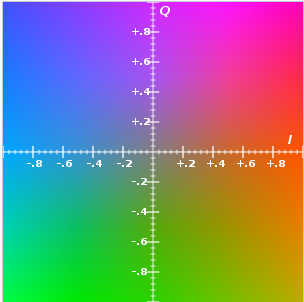
\includegraphics[width=0.4\linewidth]{./figures/yiq.png}
%	\caption{YIQ (Reproduced from\protect\cite{Various_undated-cz})}
%	\label{fig:yiq}
%\end{figure}
The $I$ component is the feature of interest here, and conversion of RGB to YIQ is achieved with this transformation:
\begin{equation}
	\begin{bmatrix}
	Y \\[0.3em]
	I \\[0.3em]
	Q \\[0.3em]
	\end{bmatrix}
	\approx
	\begin{bmatrix}
	0.299 & 0.587 & 0.114 \\[0.3em]
	0.5959 & -0.2746 & -0.3213\\[0.3em]
	0.2115 & -0.5227 & 0.3112 \\[0.3em]
	\end{bmatrix}
	\begin{bmatrix}
	R \\[0.3em]
	G \\[0.3em]
	B \\[0.3em]
	\end{bmatrix}	
\end{equation}
Here we also see convenience and ubiquity of the RGB colorspace. More often than not, color spaces are expressed as transformation from the RGB values, a technique that will be used in this section.

As Figure \ref{fig:hue_vs_inphase} shows, the tight grouping of the mean hue of an object, while interesting, is not something that can be used to predict if a plant is a weed or crop.  The in-phase component of the YIQ space, however, demonstrates a fairly clean separation that can.


\begin{figure}[H]
	\begin{subfigure}[h]{0.48\linewidth}
		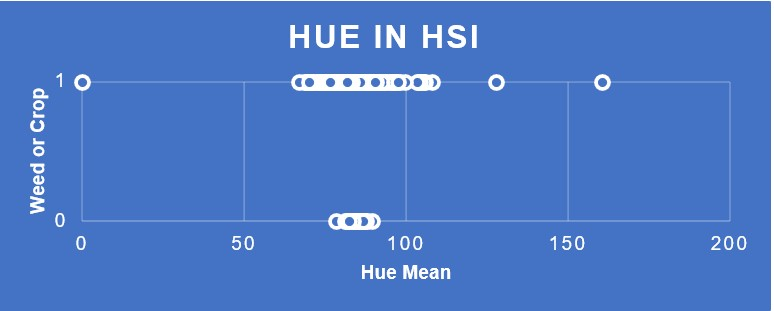
\includegraphics[width=1\linewidth]{./figures/hsi-hue.jpg}
		\caption{Hue in HSI}
		\label{subfig:hue}	
	\end{subfigure}
	\hfill
	\begin{subfigure}[h]{0.48\linewidth}
		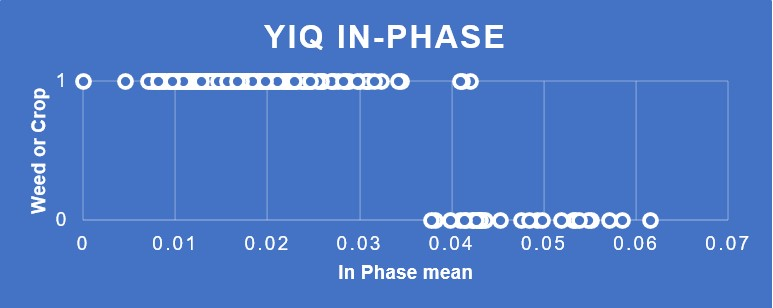
\includegraphics[width=1\linewidth]{./figures/yiq-in-phase.jpg}
		\caption{In-phase in YIQ}
		\label{subfig:in_phase}		
	\end{subfigure}%
	\caption[Prediction using hue in HSI and In-phase in YIQ]{While the grouping of hue values is certainly tighter in one group (Figure~\ref{subfig:hue}), the complete overlap between means that group assignments cannot be made with confidence. In contrast, the values of the in-phase component in the YIQ space (Figure~\ref{subfig:in_phase}) shows relatively clean separation between the two groups.}
	\label{fig:hue_vs_inphase}
\end{figure}



\subsubsection{CIElab}
Often going by the somewhat awkward acronym L*A*B*, this colorspace was intended to approximate human vision, as the L component expresses  the lightness of an object, an attribute seen a more applicable to perception of an object's color than the RGB model of mixtures of the three underlying colors.  The A and B components contain data about green to red, and blue to yellow, respectively, the four unique colors humans can perceive. While the space is not completely uniform, it is often employed in describing small changes in color. The CIElab color space was standardized in the mid-1970s but remains in widespread use today. \parencite{Wikipedia_contributors2023-xt}  The $A$ and $B$ axes are theoretically unbound, but are typically limited to some practical range, say +127 to -127. 

\begin{figure}[H]
	\centering
	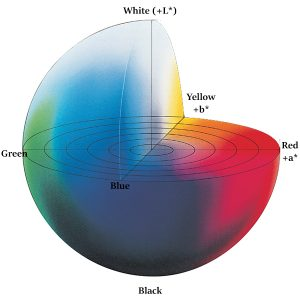
\includegraphics[width=.35\linewidth]{./figures/cielab-colorspace.jpg}
	\caption[CIElab colorspace]{In the CIElab colorspace, positive values for $b$ indicate more yellow; likewise negative values for $b$ indicate more blue. The values for $a$ similarly indicate more red (positive) or more green (negative). This is often referred to as an \textit{opponent representation} (yellow-blue and red-green) (Illustration reproduced from Color Application Specialists)}
	\label{fig:cielab}	
\end{figure}

Perceptual uniformity and pragmatic implementation details aside, the use of this colorspace is motivated by some of its salient features, most notably the ability to capture small color changes. These small color changes are expected to be significant in distinguishing crop from weed.

\subsubsection{YCbCr}
Often encountered for digital video, YCbCr encodes both luminance information ($Y$, black and white) and chrominance information ($Cb$, $Cr$). $Cb$ and $Cr$ represent the difference between a reference value and the blue or red component, respectively. This color space is similar to another encoding commonly encountered in digital video, YUV. The two spaces are nearly identical; YCbCr is a scaled version of YUV (used in analog broadcasts) This color space is also referred to by the somewhat shortened abbreviation YCC, although this document will continue to use YCbCr.

The ECMA report on the JPG file format gives this transformation for RGB to YCbCr:
\nocite{Ecma2019-yo}
\begin{equation}
	\begin{bmatrix}
	Y \\[0.3em]
	C_b \\[0.3em]
	C_r \\[0.3em]
	\end{bmatrix}
	\approx
	\begin{bmatrix}
	0.2126 & 0.7152 & 0.0722 \\[0.3em]
	-0.1146 & -0.3854 & 0.5 \\[0.3em]
	0.5 & -04542. & -0.458 \\[0.3em]
	\end{bmatrix}
	\begin{bmatrix}
	R \\[0.3em]
	G \\[0.3em]
	B \\[0.3em]
	\end{bmatrix}	
\end{equation}




\subsection{Textural}
Textural descriptors of a object are formal expressions of the relationship pixel values have with one another, reducing a tactile experience to a numerical one. Common texture descriptions, bumpy, rough, smooth, etc., refer to a quality that is useful for a human description, but tends not to be particularly exact. Each of these descriptors, however, has a few attributes in common that can then be used to quantify them relative to a fingertip: the difference between high and low points, and the spacing of these high and low points. A smooth surface could be said to have low differnce between high and low points, with small spacing. A rough surface would exhibit fairly large differences between high and low points with relatively wide spacing (at least compared to a human fingertip). While this list of descriptors is not comprehensive, and the additional quantification incomplete, this gives a sense of what is meant by a more formal texture description. Textural descriptors quantify (at least) two items: the neighborhood where a change is seen, and the direction of that change. Consider, for instance, the coat of a smooth-haired dog. Most of the hairs encountered would be aligned in the same direction, and in that direction the same texture would be encountered.
Classifying the texture is -- like color -- an analysis of the interior of the plant, and for this analysis three techniques will be used:  \textit{Grey-level Co-occurrence Matrix} (GLCM), \textit{Local Binary Pattern} (LBP) and \textit{Histogram of Oriented Gradients} (HOG). These approaches consider a pixel's relationship with surrounding pixels.

\subsubsection{GLCM}
In \textit{Grey-level Co-occurrence Matrix} (GLCM) (\cite{Haralick1973-gr}, \cite{Hall-Beyer2017-nx}), Haralick describes the analysis of an image that has been converted to greyscale values to note the relationship. Table~\ref{tab:glcm-formulae} details the subset that will be used in this analysis. The term \textit{grey-level} implies that the use of the co-occurrence matrix will be limited to greyscale images. Instead, the co-occurrence matrix will also be computed for each of the channels in the YIQ, RGB, CIELab, HSI, HSV, YCbCr colorspaces using the equations detailed in Table~\ref{tab:glcm-formulae}. For instance, the ASM calculation will be performed on the Cb channel of the image in YCbCr space. While co-occurrence matrices are used for channels in various colorspaces, this document will continue to reference the entire class as GLCM. GLCM attributes have two factors that relevant to this problem space: the distance of a pixel  considered to be a \textit{neighbor} and the angle of the relationship. Neighbor distance can be thought of as what is considered to adjacent -- the pixel immediately beside the one in question, or further away. This study considers pixels immediately adjacent to be neighbors. The angle of the relationship is a bit more complicated. While images of crops are often gathered in an orderly manner along a row such that orientation is maintained (as can be expected from a camera aboard a UAV or mounted on the back of a tractor), the vegetation is not so orderly. Otherwise identical plants are encountered in the field have markedly different texture descriptors depending on orientation. That is, different GLCM values for the same plant or obtained simply by rotating it by 45$^{\circ}$. Expressing an orientation-independent feature (texture) as differing with rotation may work well for an analysis of a single, static image set, but may yield sub-optimal results when applied to a general case where rotational differences are expected. \citeauthor*{Haralick1973-gr} discuss this, suggesting that the mean of calculations be used instead of the individual angles. 
\begin{longtable}{x{\dimexpr.15\columnwidth-2\tabcolsep}
                  x{\dimexpr.225\columnwidth-2\tabcolsep}
                  x{\dimexpr.625\columnwidth-2\tabcolsep}}
%\begin{hyphenrules}{nohyphenation}
    \caption{GLCM Formulae}\label{tab:glcm-formulae}  \\
\toprule
{\textbf{Feature}} & {\textbf{Formula}} & {\textbf{Comment}}
\tabularnewline
\midrule
    \endfirsthead
%%%%
    \caption{GLCM Features (cont.)}\label{tab:glcm-formulae}  \\
\toprule
{\textbf{Feature}} & {\textbf{Formula}} & {\textbf{Comment}}
\tabularnewline
\midrule
    \endhead
%%%%
\midrule[\heavyrulewidth]
\multicolumn{3}{r}{\footnotesize\itshape
                   Continued on the next page}
    \endfoot
%%%%
\bottomrule
    \endlastfoot
%%%%
		Homogeneity
		& \begin{minipage}[t]{0.3\textwidth}
			$\sum_{i} \sum_{j}\frac{c}{1 + \left|i-j\right|} $
		   \end{minipage}     
		& An expression of how much a pixel is similar to its neighbor
\tabularnewline\addlinespace

		Entropy     
		& $-\sum_{ij}c_{ij}\log_{2}(c_{ij}) $                    
		& An expression of how orderly the image is
\tabularnewline\addlinespace

		Correlation      
		& \begin{minipage}[t]{0.3\textwidth}
			$-\sum_{ij}\frac{(i-\mu_{i})(j - \mu_{j}) c_{ij}}{\theta_{i}\theta_{j}}$ 
		   \end{minipage}
		& An expression of the linear relationship between neighboring pixels 
\tabularnewline\addlinespace

		Dissimilarity      
		& \begin{minipage}[t]{0.3\textwidth}
			$-\sum_{ij}\frac{(i-\mu_{i})(j - \mu_{j}) c_{ij}}{\theta_{i}\theta_{j}}$ 
		   \end{minipage}
		& An expression of how much neighboring pixels differ 
\tabularnewline\addlinespace

		Contrast      
		& $\sum_{i}\sum_{j}{(i - j)}^2 c_{ij}$ 
		& Expresses the contrast between a pixel and its neighbor
\tabularnewline\addlinespace

		ASM      
		& $\sum_{ij}P{ij}^2$
		& Angular Second Moment -- high values are seen when the cell is very orderly
\tabularnewline\addlinespace

		Energy   
		& $\sqrt{ASM}$ 
		& The opposite of entropy
\label{table:glcm-formulae}
\end{longtable}

Figure~\ref{fig:glcm} illustrates an example of GLCM calculations in weed and crop images. While the clusters seen are not neatly divided, two clusters can be seen with the points sampled. This example plots the ASM and Homogeneity of grayscale images to illustrate the textural differences between plants.

\begin{figure}[H]
	\begin{subfigure}[h]{0.28\linewidth}
		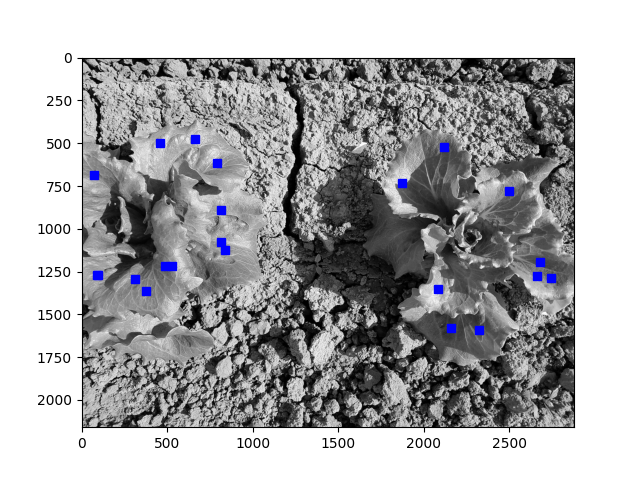
\includegraphics[height=5cm]{./figures/glcm-crop.png}
		\caption{Lettuce}
		\label{subfig:glcm_crop}	
	\end{subfigure}
	\hfill
	\begin{subfigure}[h]{0.28\linewidth}
		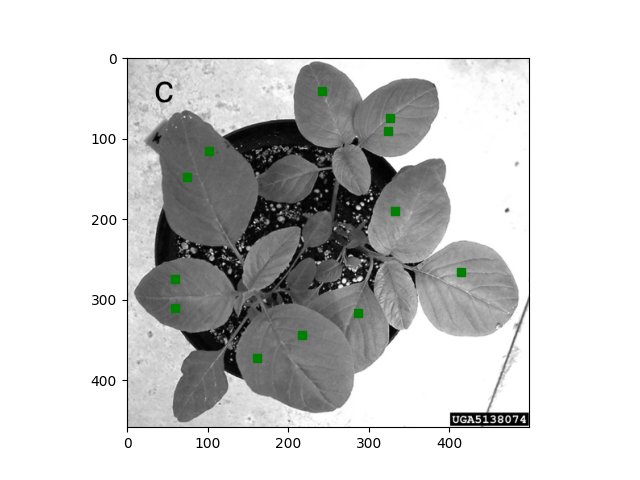
\includegraphics[height=5cm]{./figures/glcm-weed.png}
		\caption{Pigweed}
		\label{subfig:glcm_weed}		
	\end{subfigure}%
	\hfill
	\begin{subfigure}[h]{0.28\linewidth}
		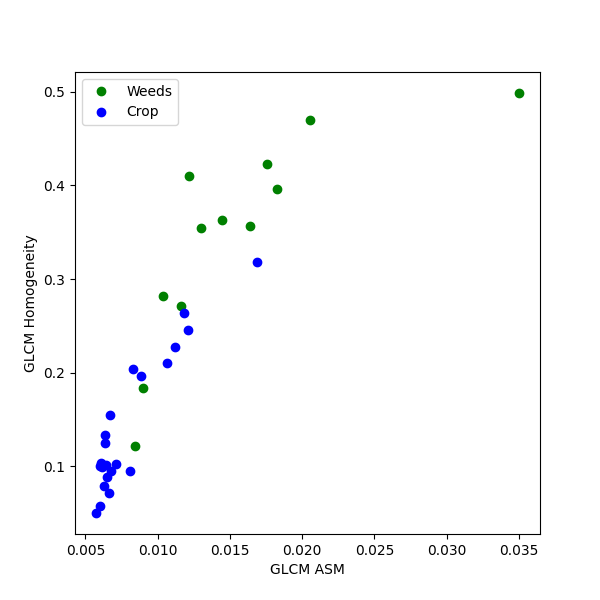
\includegraphics[height=5cm]{./figures/glcm-plot.png}
		\caption{ASM \& Homogenity}
		\label{subfig:glcm_plot}		
	\end{subfigure}%
	\hfill
	\caption[An example of GLCM calculations for weed and crop]{GLCM calculations derived from crop (\ref{subfig:glcm_crop}) and weed (\ref{subfig:glcm_crop}) show that the sampled points in weeds (green dots) and crop (blue dots) fall into two clusters. While this does not account for differences in lighting conditions or resolution between the two images, this illustrates the expected textural differences between the two plant types that are more easily seen (``weeds just look like they would feel different than crops''), than quantified. Crop image source: Dr. Mark Siemens, University of Arizona. Weed image source: University of California Agriculture and Natural Resources}
	\label{fig:glcm}
\end{figure}

While the term \textit{Grey Level} is often applied to this technique (and will be used throughout this document with the GLCM abbreviation), the technique will be applied not just to images converted from the RGB colorspace to greyscale, but to the various colorspaces previously discussed. The calculations will be made on each component of those spaces.  That is, each of the seven calculations are made for each component of the various color spaces (YIQ, HSI, etc.). If computations are made for each of the angles (0$^{\circ}$, 45$^{\circ}$, 90$^{\circ}$, 135$^{\circ}$, 180$^{\circ}$) as well as the average the resulting output of many hundreds of calculations is more than can be comfortably presented here. These computations, however, will be presented in subsequent sections, taking the form \textit{$<$colorspace$>$\_$<$component$>$\_$<$glcm-calculation$>$\_$<$angle$>$}, i.e., \textit{yiq\_i\_energy\_135} to indicate the energy computation at 135$^{\circ}$ of the in-phase component of the blob in the YIQ colorspace.

\begin{figure}[H]
	\centering
	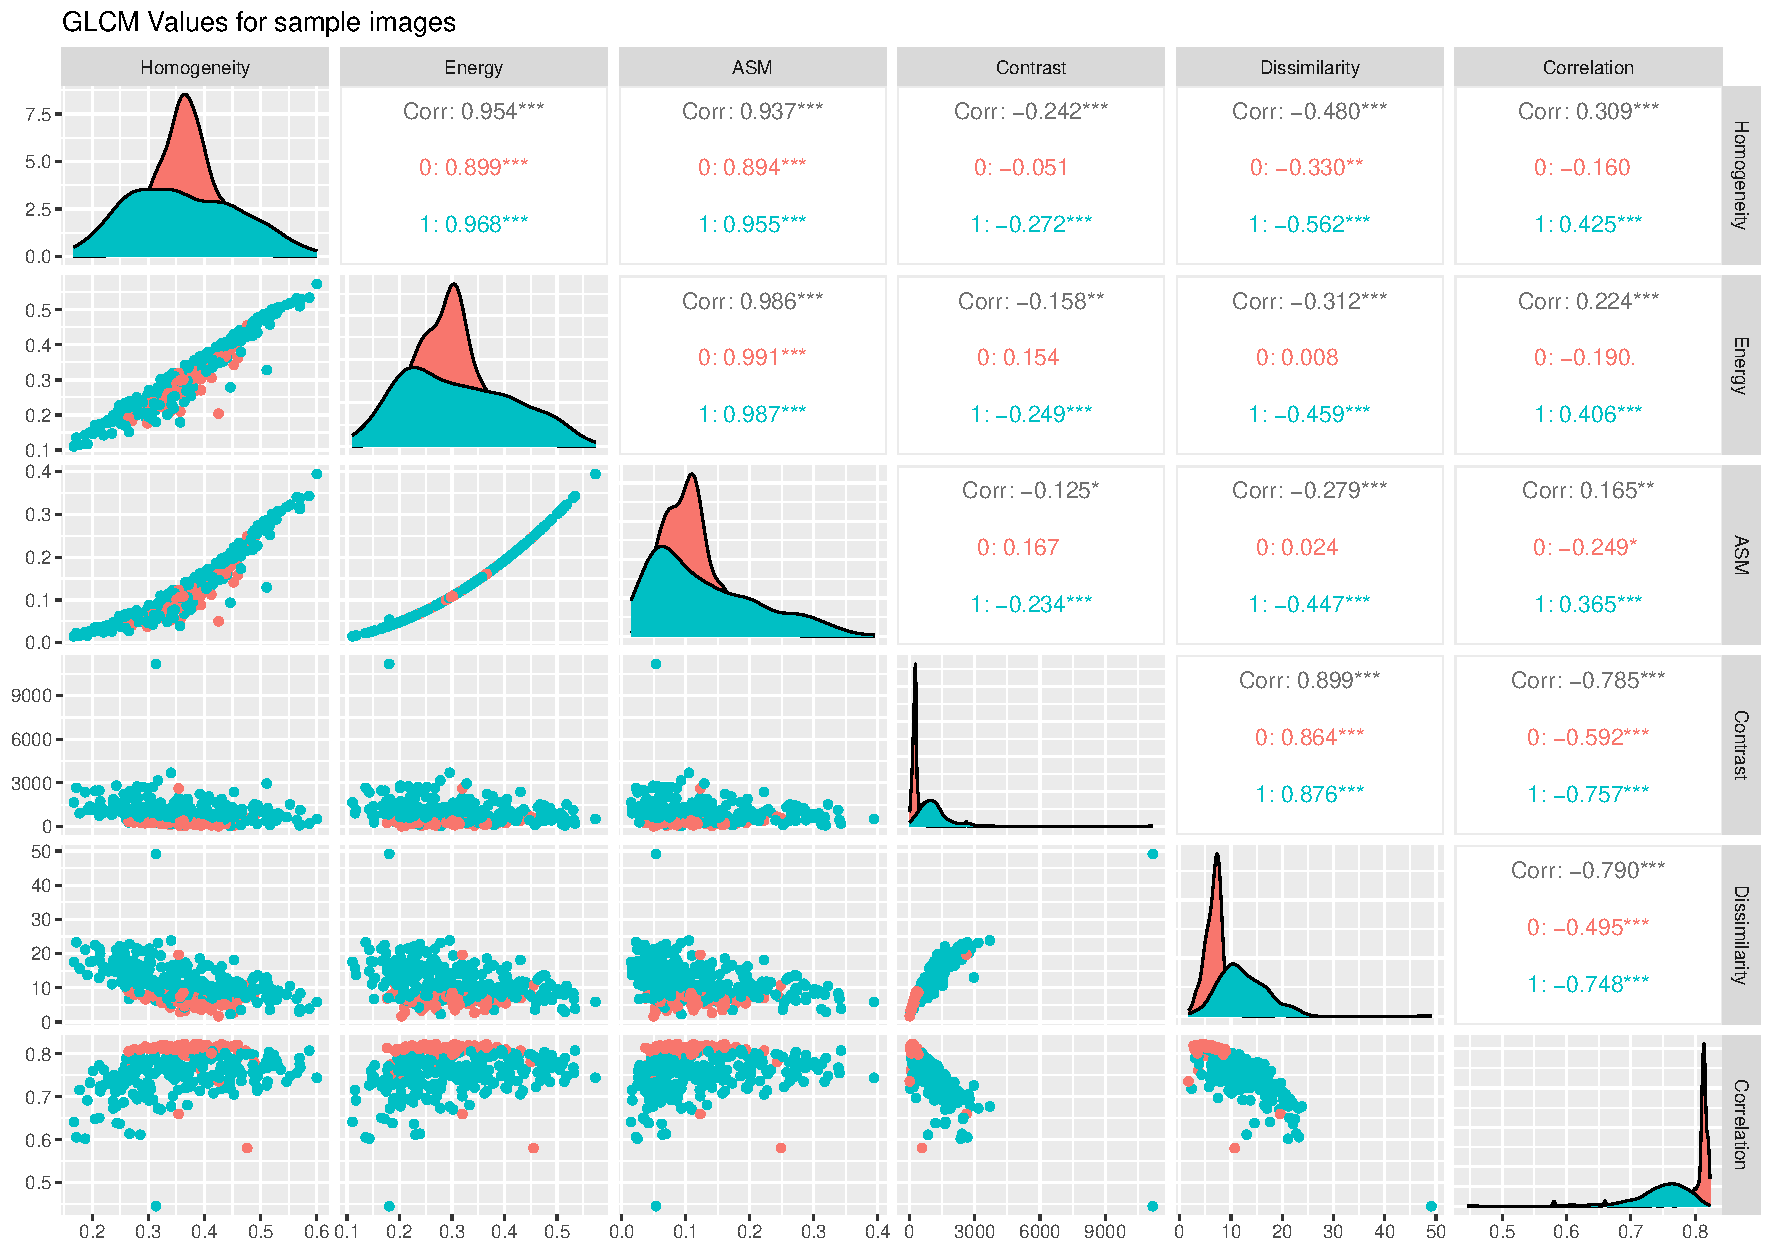
\includegraphics[width=0.9\linewidth]{./figures/glcm-pairs.pdf}
	\caption[GLCM parameter correlation assessment]{A breakdown of the GLCM parameter calculations detailed in Table~\ref{table:glcm-formulae} for the sample images (greyscale). In contrast to the samples within an image demonstrated by Figure~\ref{fig:glcm}, these calculations are carried out across the entire plant. To negate the distortions seen with specific orientations of vegetation, these are averages across the entire plant, not specific angles. Some of the relationships are interrelated, so the data may look much more interesting than it actually is. \textit{Energy}, for instance, is the square root of \textit{ASM}, so no special significance should be attributed to that curve presented above. For the purposes of exploring the data, it is not of particular concern what class 0 and 1 represent.}
\end{figure} 

\subsubsection{Local Binary Pattern}
Often shortened to LBP, \citeauthor{Ojala1996-ps} first described Local Binary Patterns, concentrating on a pixel's immediate neighbors, and treating the result as a value that can be thought of as describing that central pixel. While first proposed as a texture descriptor, its use in more general computer vision problems has expanded since it was first introduced. However useful this approach is, it does have a hard limitation: only a 3x3 matrix can be used to produce the final value. This is more of a limitation than it first appears, as this technique is not suitable for capturing details at varying scales.

\begin{figure}[H]
	\begin{subfigure}[h]{0.48\linewidth}
		\centering
		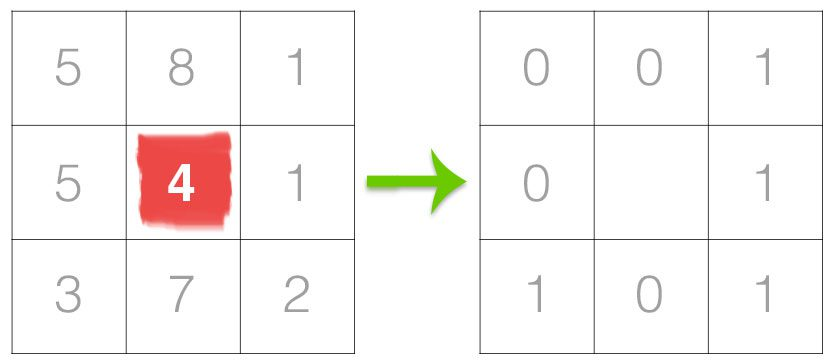
\includegraphics[height=2cm]{./figures/lbp_thresholding.jpg}
		\caption{LBP Thresholding}
		\label{subfig:lbp-thresholding}	
	\end{subfigure}
	\hfill
	\begin{subfigure}[h]{0.48\linewidth}
		\centering
		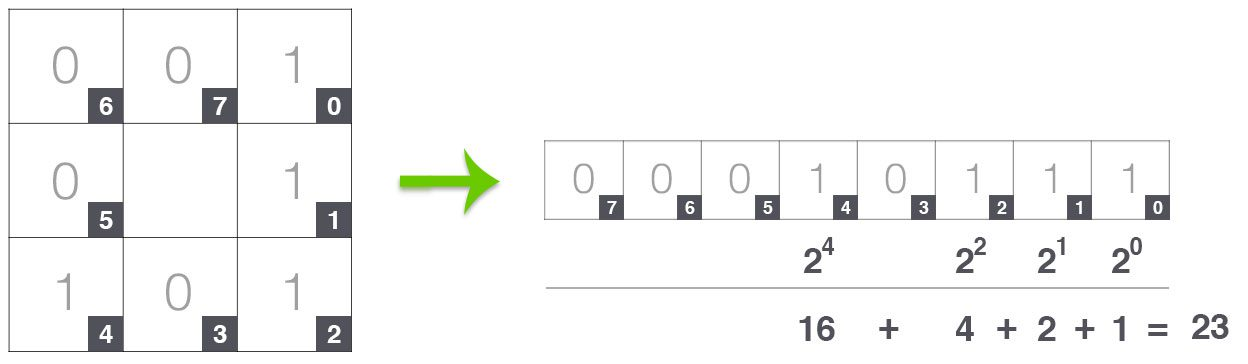
\includegraphics[height=2cm]{./figures/lbp_calculation.jpg}
		\caption{LBP Calculation}
		\label{subfig:lbp-calculation}		
	\end{subfigure}%
	\caption[Local Binary Pattern thresholding and calculation]{To determine the LBP value of the central pixel (marked in red in \ref{subfig:lbp-thresholding}), the value is thresholded to produce the second matrix: where the original matrix has a value $<$ 4 the original value is replaced with a 0. Values greater than 4 are replaced by a 1. This result matrix is then used as the binary values of a single integer, 23 in this example. Considering a 3x3 matrix, there are $2^8$ possibilities. (Images reproduced from PyImageSearch)}
	\label{fig:lbp}
\end{figure}

To make this technique more useful, a variant of this is used, where a circular neighborhood is considered instead of a square. The radius of the circle allows consideration of features at different scales.  Subsets of an image can then be described by moving the square or circular neighborhood across the image.  Sampling in a circular pattern will mean that some samples will not be be between two pixels. In this case, the intensity value used for the comparison can be determined by bilinear interpolation. This sampling discrepancy between a pixel's center and the actual sampling point can be seen in the middle neighborhood diagram of Figure ~\ref{fig:lbp-circular}, where pixel centers and sampling points are not aligned in many instances.

\begin{figure}[H]
	\centering
	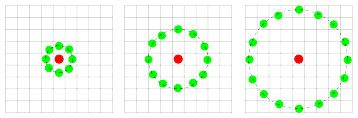
\includegraphics[height=2cm]{./figures/lbp_circular.jpg}	
	\caption[Local Binary Pattern circular neighborhoods]{The size of a neighborhood can be varied depending on the size of the detail to be characterized. The neighborhood on the left roughly corresponds to the 8 position square neighborhood seen in Figure \ref{fig:lbp} (Image reproduced from PyImageSearch)}
	\label{fig:lbp-circular}
\end{figure}

An introduction to LBP concepts would not be complete without addressing the notion of \textit{LBP Uniformity}. An LBP is considered to be uniform if it has at most two $0 \rightarrow 1$ or $1 \rightarrow 0$ transitions in the binary representation. The LBP pattern $01000000$ shows one $0 \rightarrow 1$ transition and one $1 \rightarrow 0$ transition, making it uniform. A pattern such as $01010000$ would not be considered uniform, as there are more than two transformations. This 


\subsubsection{Histogram of Oriented Gradients}
Often shortened to \textit{HOG}, this technique is a technique to formalize the gradient orientation and magnitude of local portions of an image \parencite[p.~155]{Forsyth2012-hy}. This is a structural analysis that gives insight to not only the overall shape of the object, but to the interior details as well, as this technique is geared toward the identification of high-contrast edges within the object. Contrast this with the shape analysis detailed earlier in the document where the concern was limited almost exclusively to the perimeter of the vegetation.  As shape analysis considers only the edge of the blob, the vegetation is effectively a cartooned image, providing only areas of black and white. This technique considers small cells within an image, lowering the risk that a gradient with low contrast will be missed, as it will be compared (and normalized) within that small cell. While much of the literature on this topic focuses on describing an entire scene, that is not the case here, as the background has been eliminated and the object in question is known to be vegetation.
The detail shown in Figure~\ref{fig:hog} is still recognizable as vegetation, but illustrates gradient orientation of 16x16\footnote{The cell size can be varied, of course. This size was selected somewhat arbitrarily} cells of the image, not pixel values. It is these orientations that will be exploited in classification.  For the classification approach described in this document, the gradients will be reduced to a few numbers to describe each plant. Specifically the mean, standard deviation, and the range of the magnitudes of the gradient descriptors for a plant. In lettuce the orientation of a gradient is visible even to the unaided eye, as the vein structure can be used to classify the image \parencite{Elhariri2014-eo}. While detailed analysis of structures will not be directly used in classification, the overall effect of those structures will be used. That is, to say that leaf is ``very veiny'' or ``quite rough'' can be quantified with a few numbers that are reflective of the overall texture of the plant.
\begin{figure}[H]
	\centering
	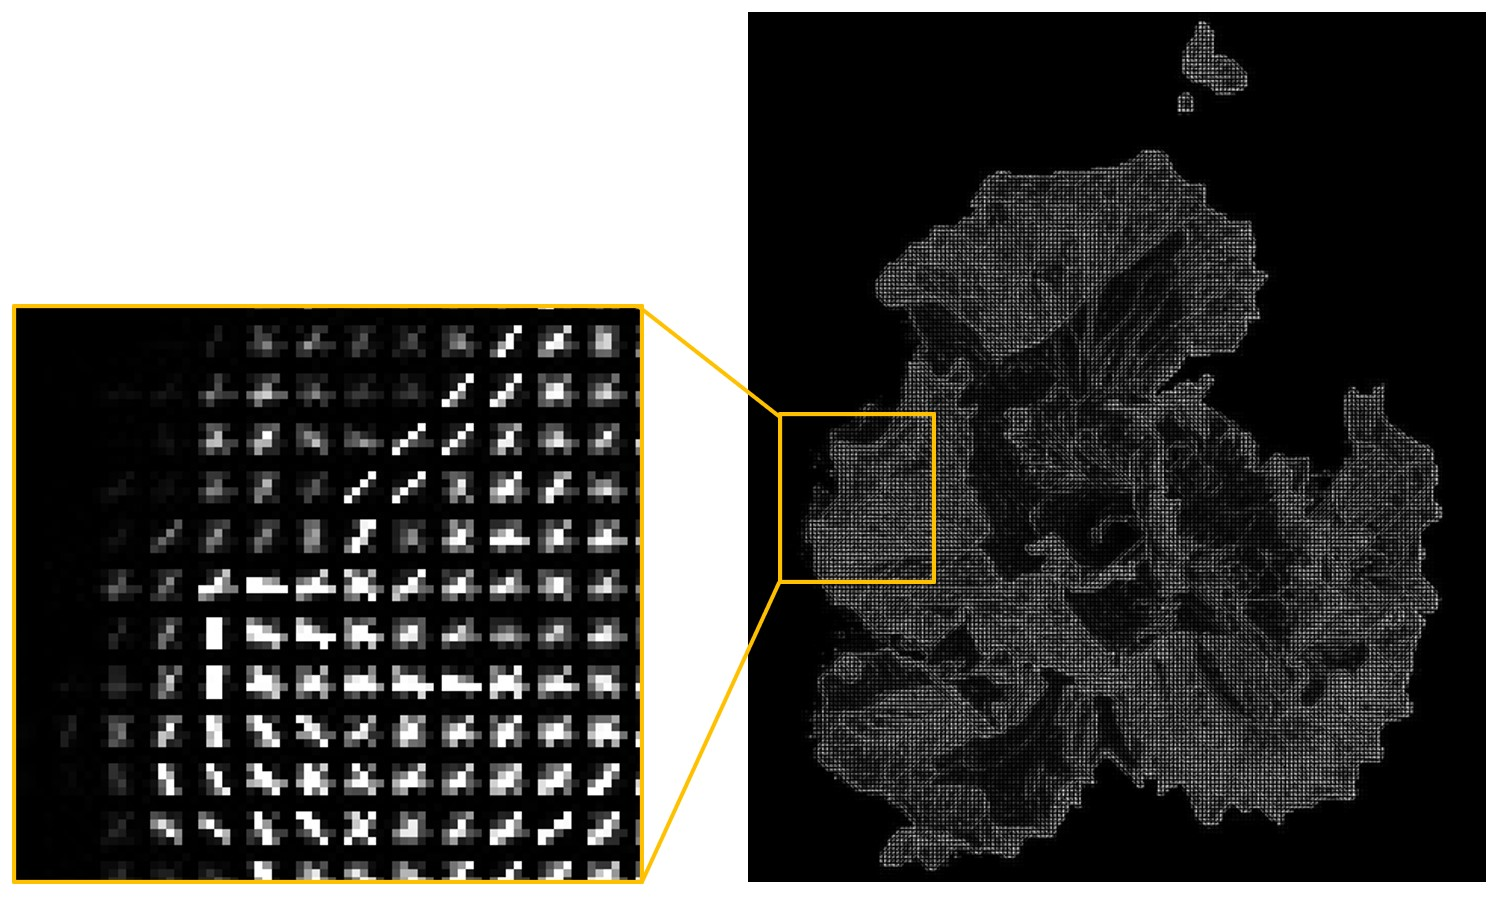
\includegraphics[width=0.4\linewidth]{./figures/hog.jpg}
	\caption[HOG Representation of Lettuce]{HOG Representation of greyscale lettuce image. This image represents not the actual pixels of the image, but is a representation of the gradients found within each 16x16 cell.}
	\label{fig:hog}
\end{figure}

\begin{figure}[h!]
	\centering
	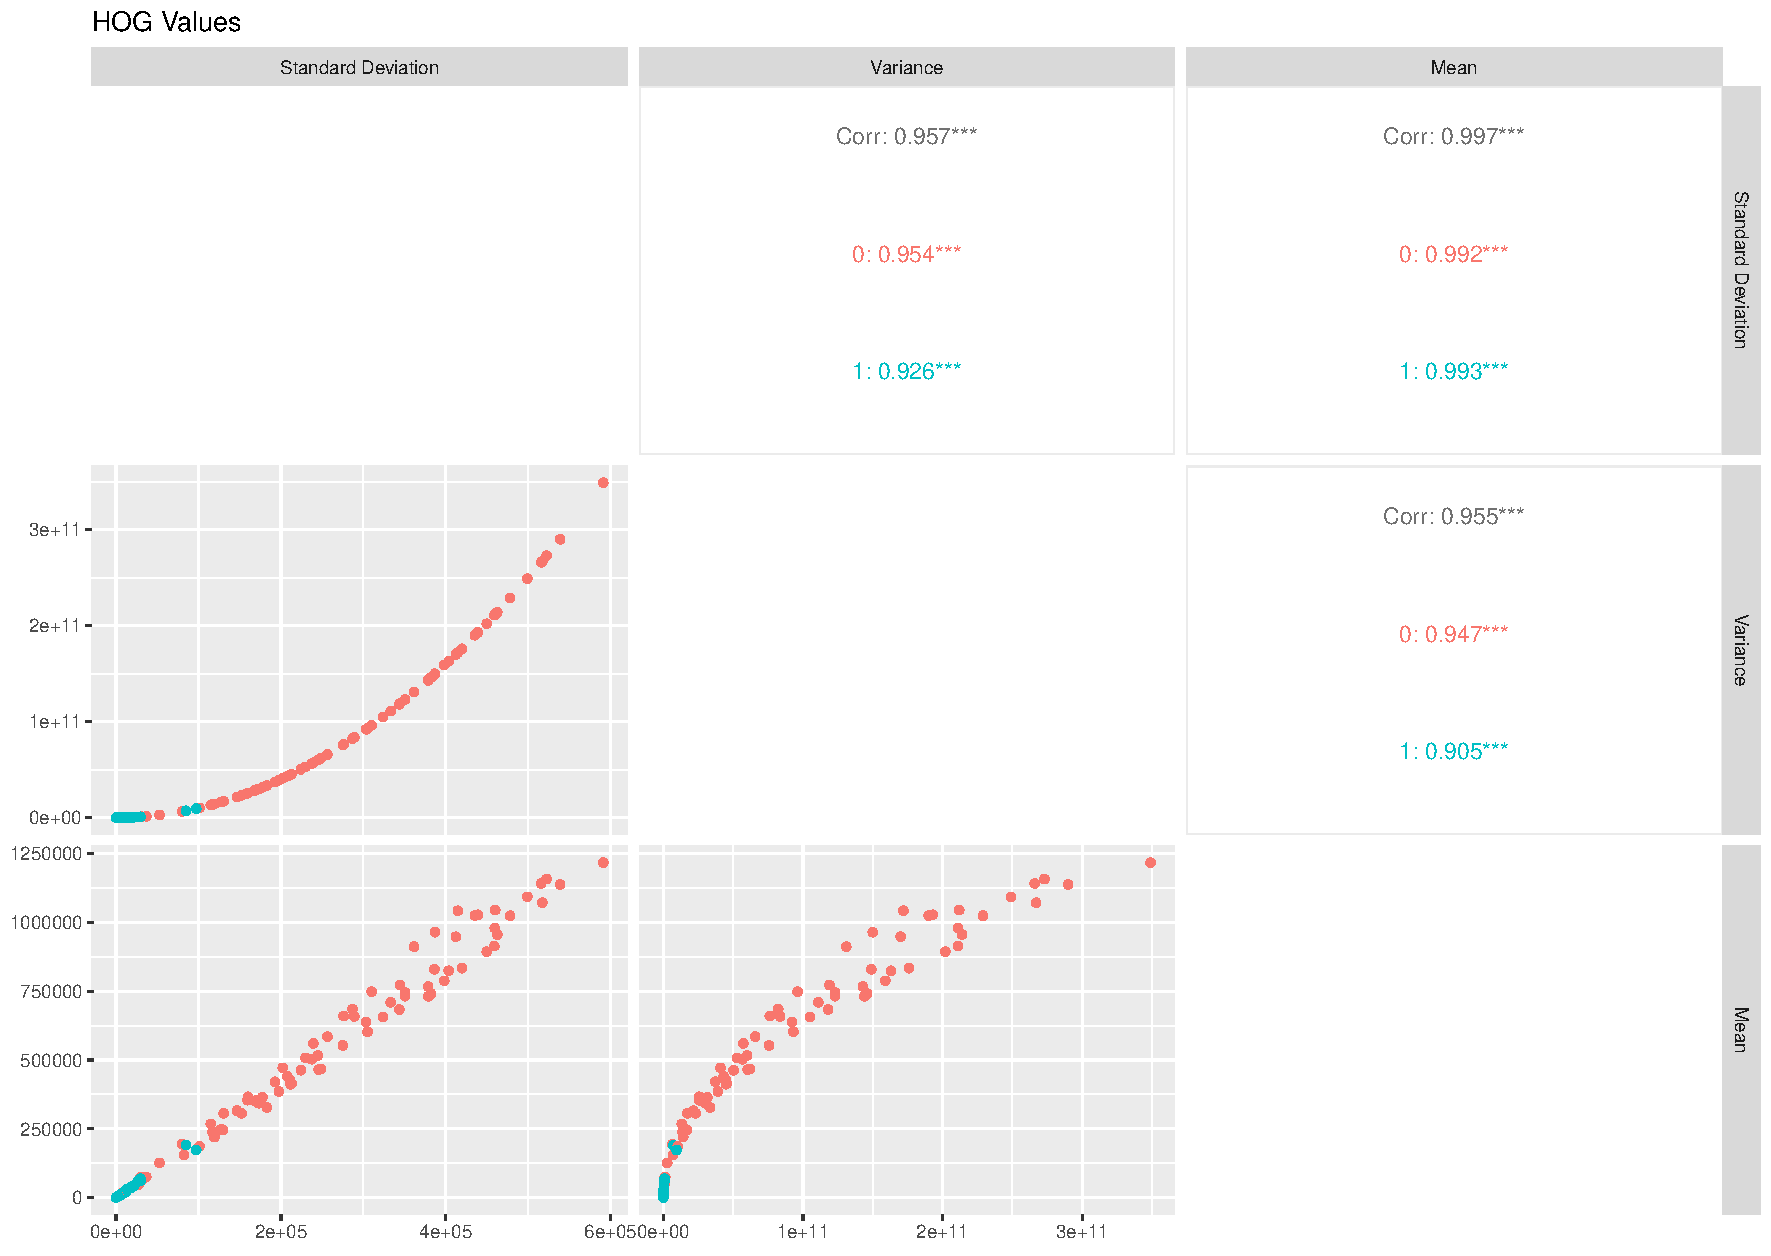
\includegraphics[width=0.7\linewidth]{./figures/hog-pairs.pdf}
	\caption[HOG features used in classification]{Instead of considering the values of small cells contained within the perimeter of the blob, the classification will use attributes of that portion of the image. That is, the measurements shown in this figure are for the blob in question, not for the image as a whole. For the purposes of exploring the data, it is not of particular concern what class 0 and 1 represent.}
	\label{fig:hog-pairs}
\end{figure}

 

\subsection{Distance from Cropline}
The cropline in a planting is, simply, the line along the bed where crop can be expected. Under field conditions where images are acquired from a constant position the cropline will appear in the same spot in each photo. For classification purposes, the idea is obvious to anyone who has had the pleasure of performing weeding along a cropline: things along the cropline are likely to be crop, and things not along the cropline are likely to be weeds. Things are a bit more complicated than that, of course, and it is probably more accurate to use the terms \textit{desired} and \textit{undesired} to classify vegetation. Weeds may appear along the cropline or within close proximity to crop\footnote{The concept of a defining a buffer zone around crop to avoid damage during treatment will be discussed later in this document}, and crop may appear in places other than the main cropline, making it \textit{undesirable}, but referring to it as a weed would lead to confusion.

Crops will most often have a distance from the cropline very close to zero. Weeds, on the other hand, may have a distance close to zero if they appear within the line of crop, but often appear far from the crop line.
\begin{figure}[h!]
	\centering
	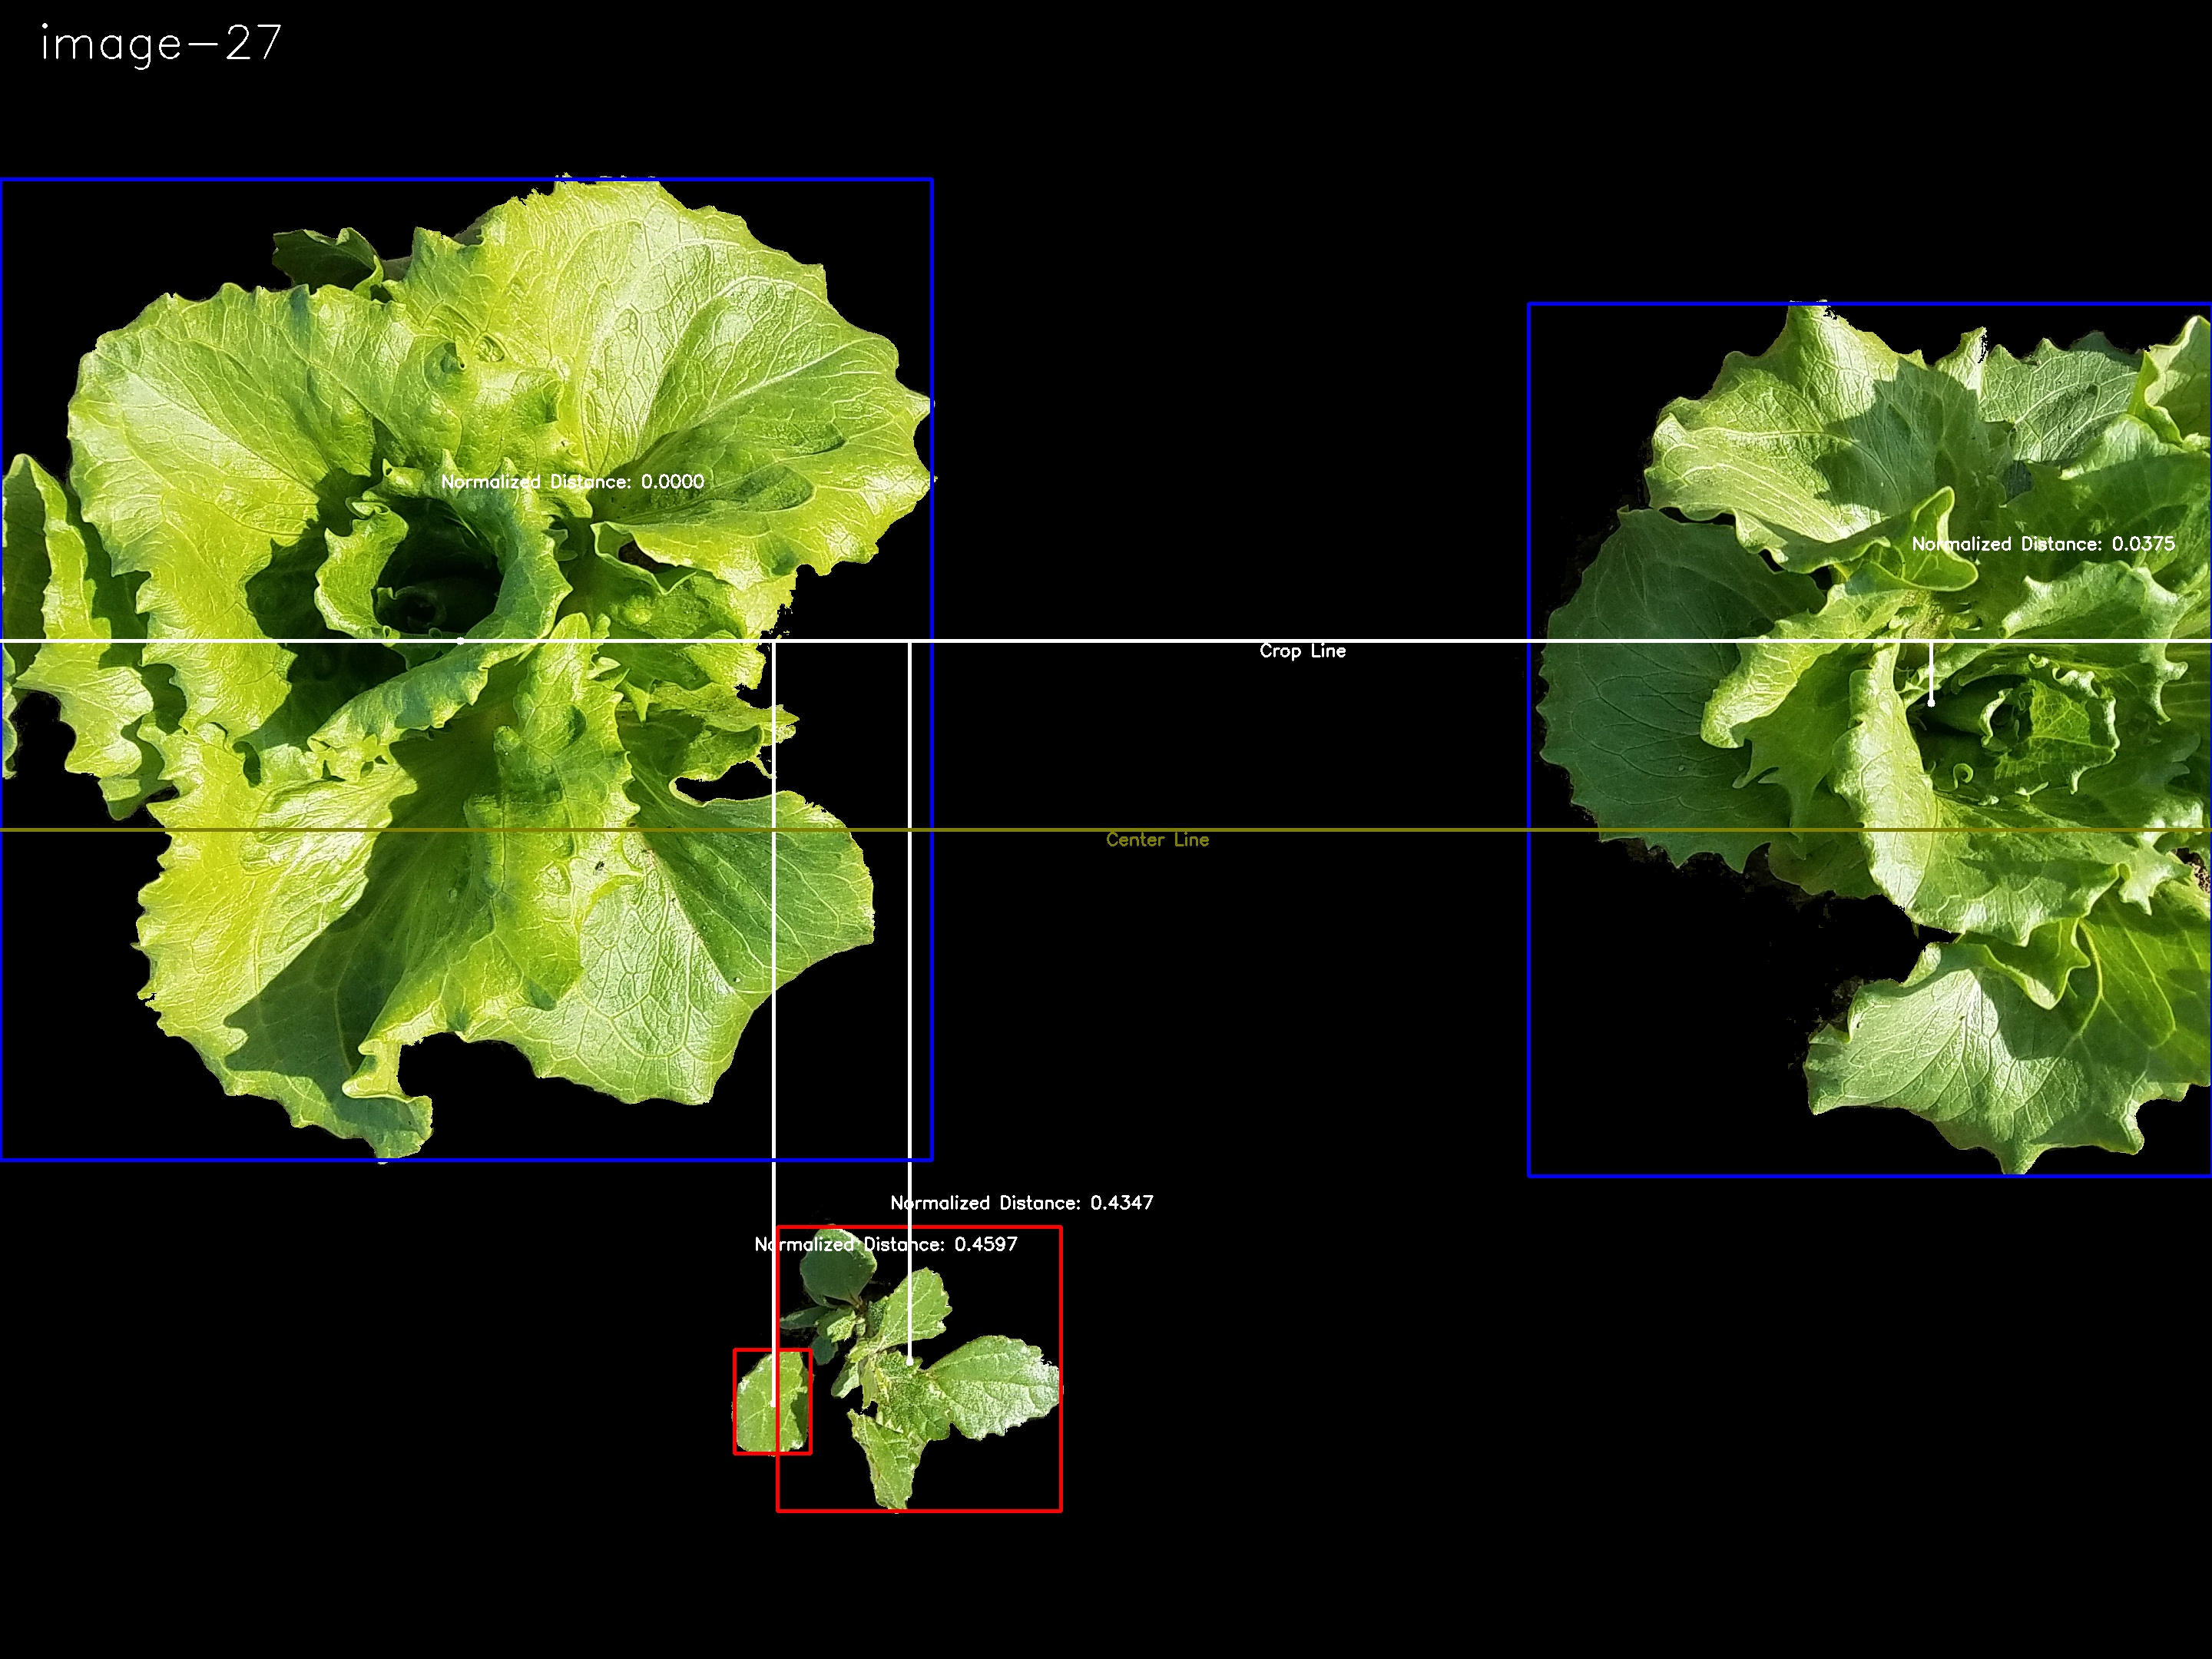
\includegraphics[width=0.4\linewidth]{./figures/normalized-distance.jpg}
	\caption[Distance from Cropline]{Distance from Cropline. Vegetation far from the cropline are most often weeds.}
	\label{fig:normalized-distance}
\end{figure}
Figure~\ref{fig:normalized-distance} illustrates the concept of a cropline and the distance of vegetation from it. In this image we see two growths of lettuce that are very close to the cropline (distances here are in pixels, but the units are not significant. This could be expressed in millimeters) at 0 and 0.375 and a weed lying 0.4347 units from the cropline. The values normalized between 0 and 1 by considering the maximum distance the vegetation could be away from the crop line. The line marked \textit{Center Line} is for reference purposes and can be ignored for now.  There are two additional items that are worth noting about this image: the dots connecting the plant to the cropline are the {\it centroids} mentioned earlier, and the colored bounding boxes signify the class of the object, something we will return to in a later section.

While images obtained in close proximity to the planting beds may contain only a single cropline, images contained from higher distances AGL will often contain multiple croplines. In the former case, it is often the case that fairly simple metrics can be used to determine the cropline -- size ratios between vegetation.  The line connecting the two largest plants, for instance, is, more often than not, the cropline. This is the case, however, only for those images taken from very low distances above ground (40 cm or so) where the image contains only a single row. For imagery taken from higher distances AGL, a different approach is called for. \citeauthor*{Dian_Bah2017-kd} discuss the use of a Hough Transform \parencite{Illingworth1988-nw} to identify planting rows in AUV imagery; a technique that will be used here. \citeauthor{Ji2011-qb} analyse Hough transforms and \textit{random} hough transforms \parencite{Ji2011-qb} for three different plant densities, showing that the random hough transform was more computational efficient than a simple hough transform.

\begin{figure}[h!]
	\centering
	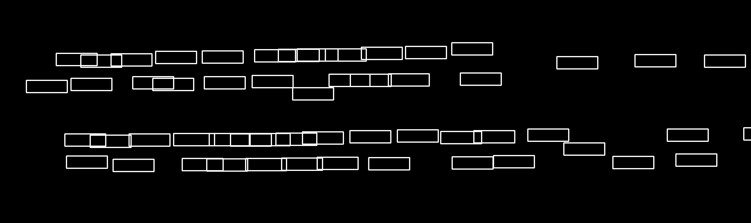
\includegraphics[width=0.8\linewidth]{./figures/hough-transform-rectangles.jpg}
	\caption[Rectangles for hough transform]{Rather than perform a hough transform on the raw image of the vegetation, each plant is first transformed into a series of rectangles, the center of which is the centroid of each plant. }
	\label{fig:hough-transform}
\end{figure}



\subsection{Overlapping Vegetation}
\label{problem-overlap}

Before considering the details of classification, it is worth considering a problem that is sometimes seen: overlapping vegetation. While vegetation can overlap itself (in that leaves may obscure other leaves in the same plant), this becomes problematic when desired and undesired vegetation overlap, creating the appearance of two plants being seen as one. Normal overlap within a plant's leaves renders edge detection ineffective in this instance -- that is, distinguishing between expected, normally occurring overlap within a plant's leaves, and overlap between plants is problematic. Overlapping vegetation is problematic in the current processing flow, as a plant is identified by the pixels within a contiguous  perimeter. In this case it is detected as part of the adjoining vegetation, distorting the calculations detailed in previous sections.  Consider this portion of an image:
\begin{figure}[H]
	\centering
	\begin{subfigure}[h]{.45\textwidth}
		\centering
		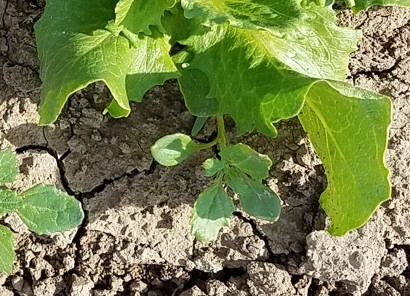
\includegraphics[width=6cm]{./figures/overlapping-weed.jpg}
		\caption{Raw image}
		\label{fig:overlap-raw}
	\end{subfigure}
	\hfill
	\begin{subfigure}[h]{.45\textwidth}
		\centering
		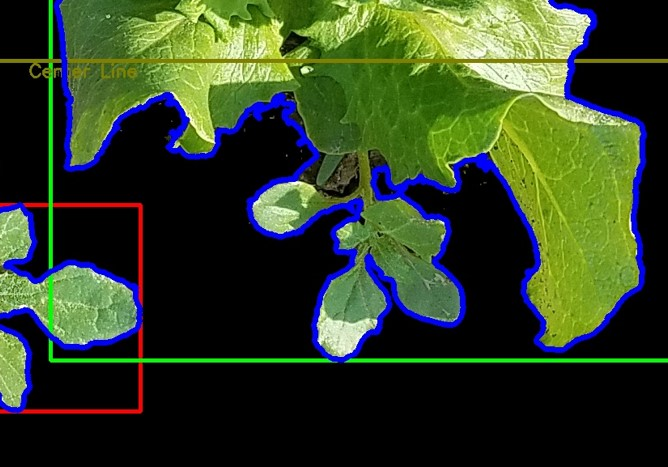
\includegraphics[width=6cm]{./figures/overlapping-weed-segmented.jpg}
		\caption{Segmented image}
		\label{fig:overlap-segmented}
	\end{subfigure}
	\caption[Crop and Weed overlap]{Crop and Weed overlap -- this image contains a problem commonly encountered, the situation where there is overlap between the crop and weeds. In this instance, the crop partially obscures the weed. The blob detection algorithm does not use factors such as color differences to distinguish one blob from another, resulting in two plants being processed as a single one, as can be observed in~\ref{fig:overlap-segmented}. As the weed has been falsely identified as belonging to the crop, its characteristics contribute to the overall calculations for the blob. Most notably, the shape is distorted, but this also affects color and texture calculations.}
	\label{fig:overlap}
\end{figure}


The object detection algorithms are based on shapes of binary images, leading to the case where a few leaves of the weed are incorrectly identified as part of the crop. In this case,some leaves are identified as separate plants and are marked as requiring treatment, but this may not be the case with a larger plant requiring treatment that happens to overlap with desired vegetation. This affects not only the inclusion of weeds with crop, but the misidentification of several weeds as a single plant, as this image demonstrates.  Two of the plants in the image are identified as a single blob as the overlapping leaves of multiple plants makes it appear as one. While this a mistake that will result in the distortion of metrics, the weed occupies a space so close to the crop that it would not be treated even if properly identified.

\subsection{Weed Shapes and Color}
There are two complications with the identification of weeds by considering shape.  Computation of the shape index of objects within the image are complicated by poor lighting requiring more pixel dilation to make the vegetation appear to be a single plant. This, in turn, distorts the computation of the shape index of the object. The indices covered in Table~\ref{table:segmentation} fail to capture elements of the vegetation that are other than the commonly encountered green.

Consider a sample of Purslane detailed in Figure~\ref{fig:segmentation-problem}. As the red stems are not detected by the green-centric index, the resulting segmented image appears to show multiple plants where there is only one.

\begin{figure}[h!]
	\centering
	\begin{subfigure}[h]{.40\textwidth}
		\centering
		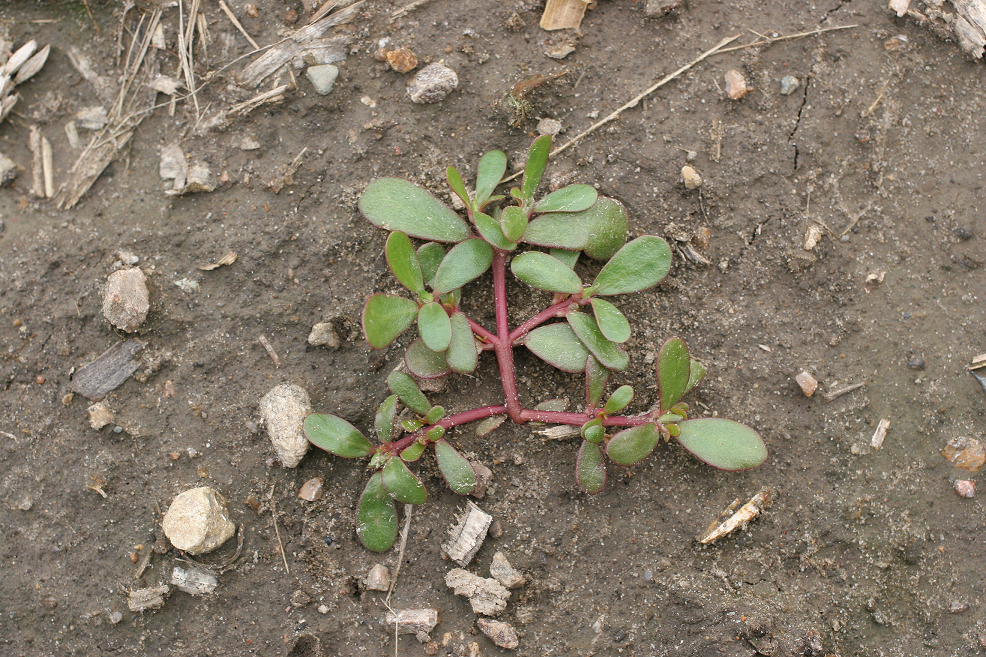
\includegraphics[width=6cm]{./figures/purslane.png}
		\caption{Purslane}
		\label{fig:purslane}
	\end{subfigure}
	\begin{subfigure}[h]{.40\textwidth}
		\centering
		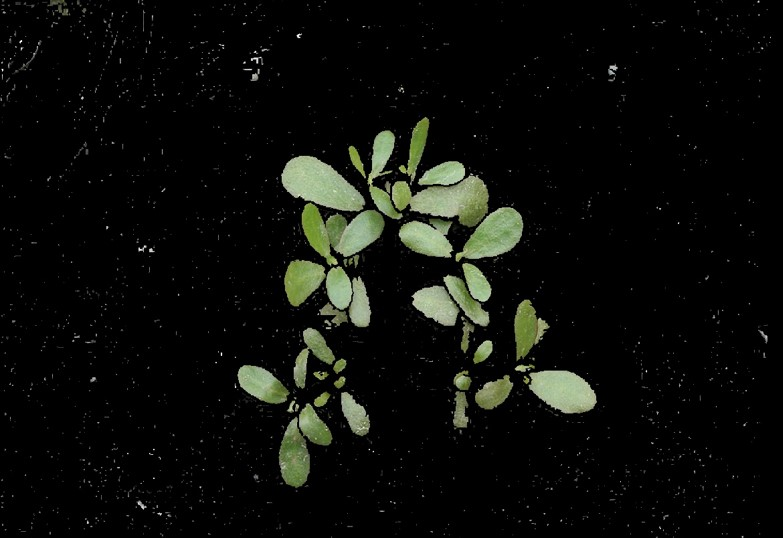
\includegraphics[width=6cm]{./figures/purslane-segmented.jpg}
		\caption{Segmented image (NDI)}
		\label{fig:purslane-segmented}
	\end{subfigure}
	\caption[Color problems complicate segmentation]{The red stems found in purslane complicate use of indices calculated to emphasize green vegetation. As seen in Figure~\ref{fig:purslane-segmented}, the prominent red stems are not present in the final image.}
	\label{fig:segmentation-problem}
\end{figure}

Even weeds that are predominantly green have portions that are less green than others. The color of the purslane stem is a shade of red that is not isolated by considering only a single threshold of the vegetation indices discussed earlier in this document. While using a second threshold value to capture the stems is an option, this approach is complicated by the red content of the background -- the ground may have a significant red hue, a situation not frequently encountered with green vegetation. This problem is not unique to purslane, but can be seen in other vegetation with significant amounts of red in edges of leaves such as found in redroot pigweed (\textit{Amaranthus retroflexus}).  The presence of red in leaves mis-identification of leaves as separate plants (stems) and to the distortion of shape metrics (leaves). While this tends toward a negative impact on calculations that involve the entire plant, calculations involving only the leaves does not appear to have detrimentally affect classification.

%\begin{figure}[h!]
%	\centering
%	\begin{subfigure}[h]{.40\textwidth}
%		\centering
%		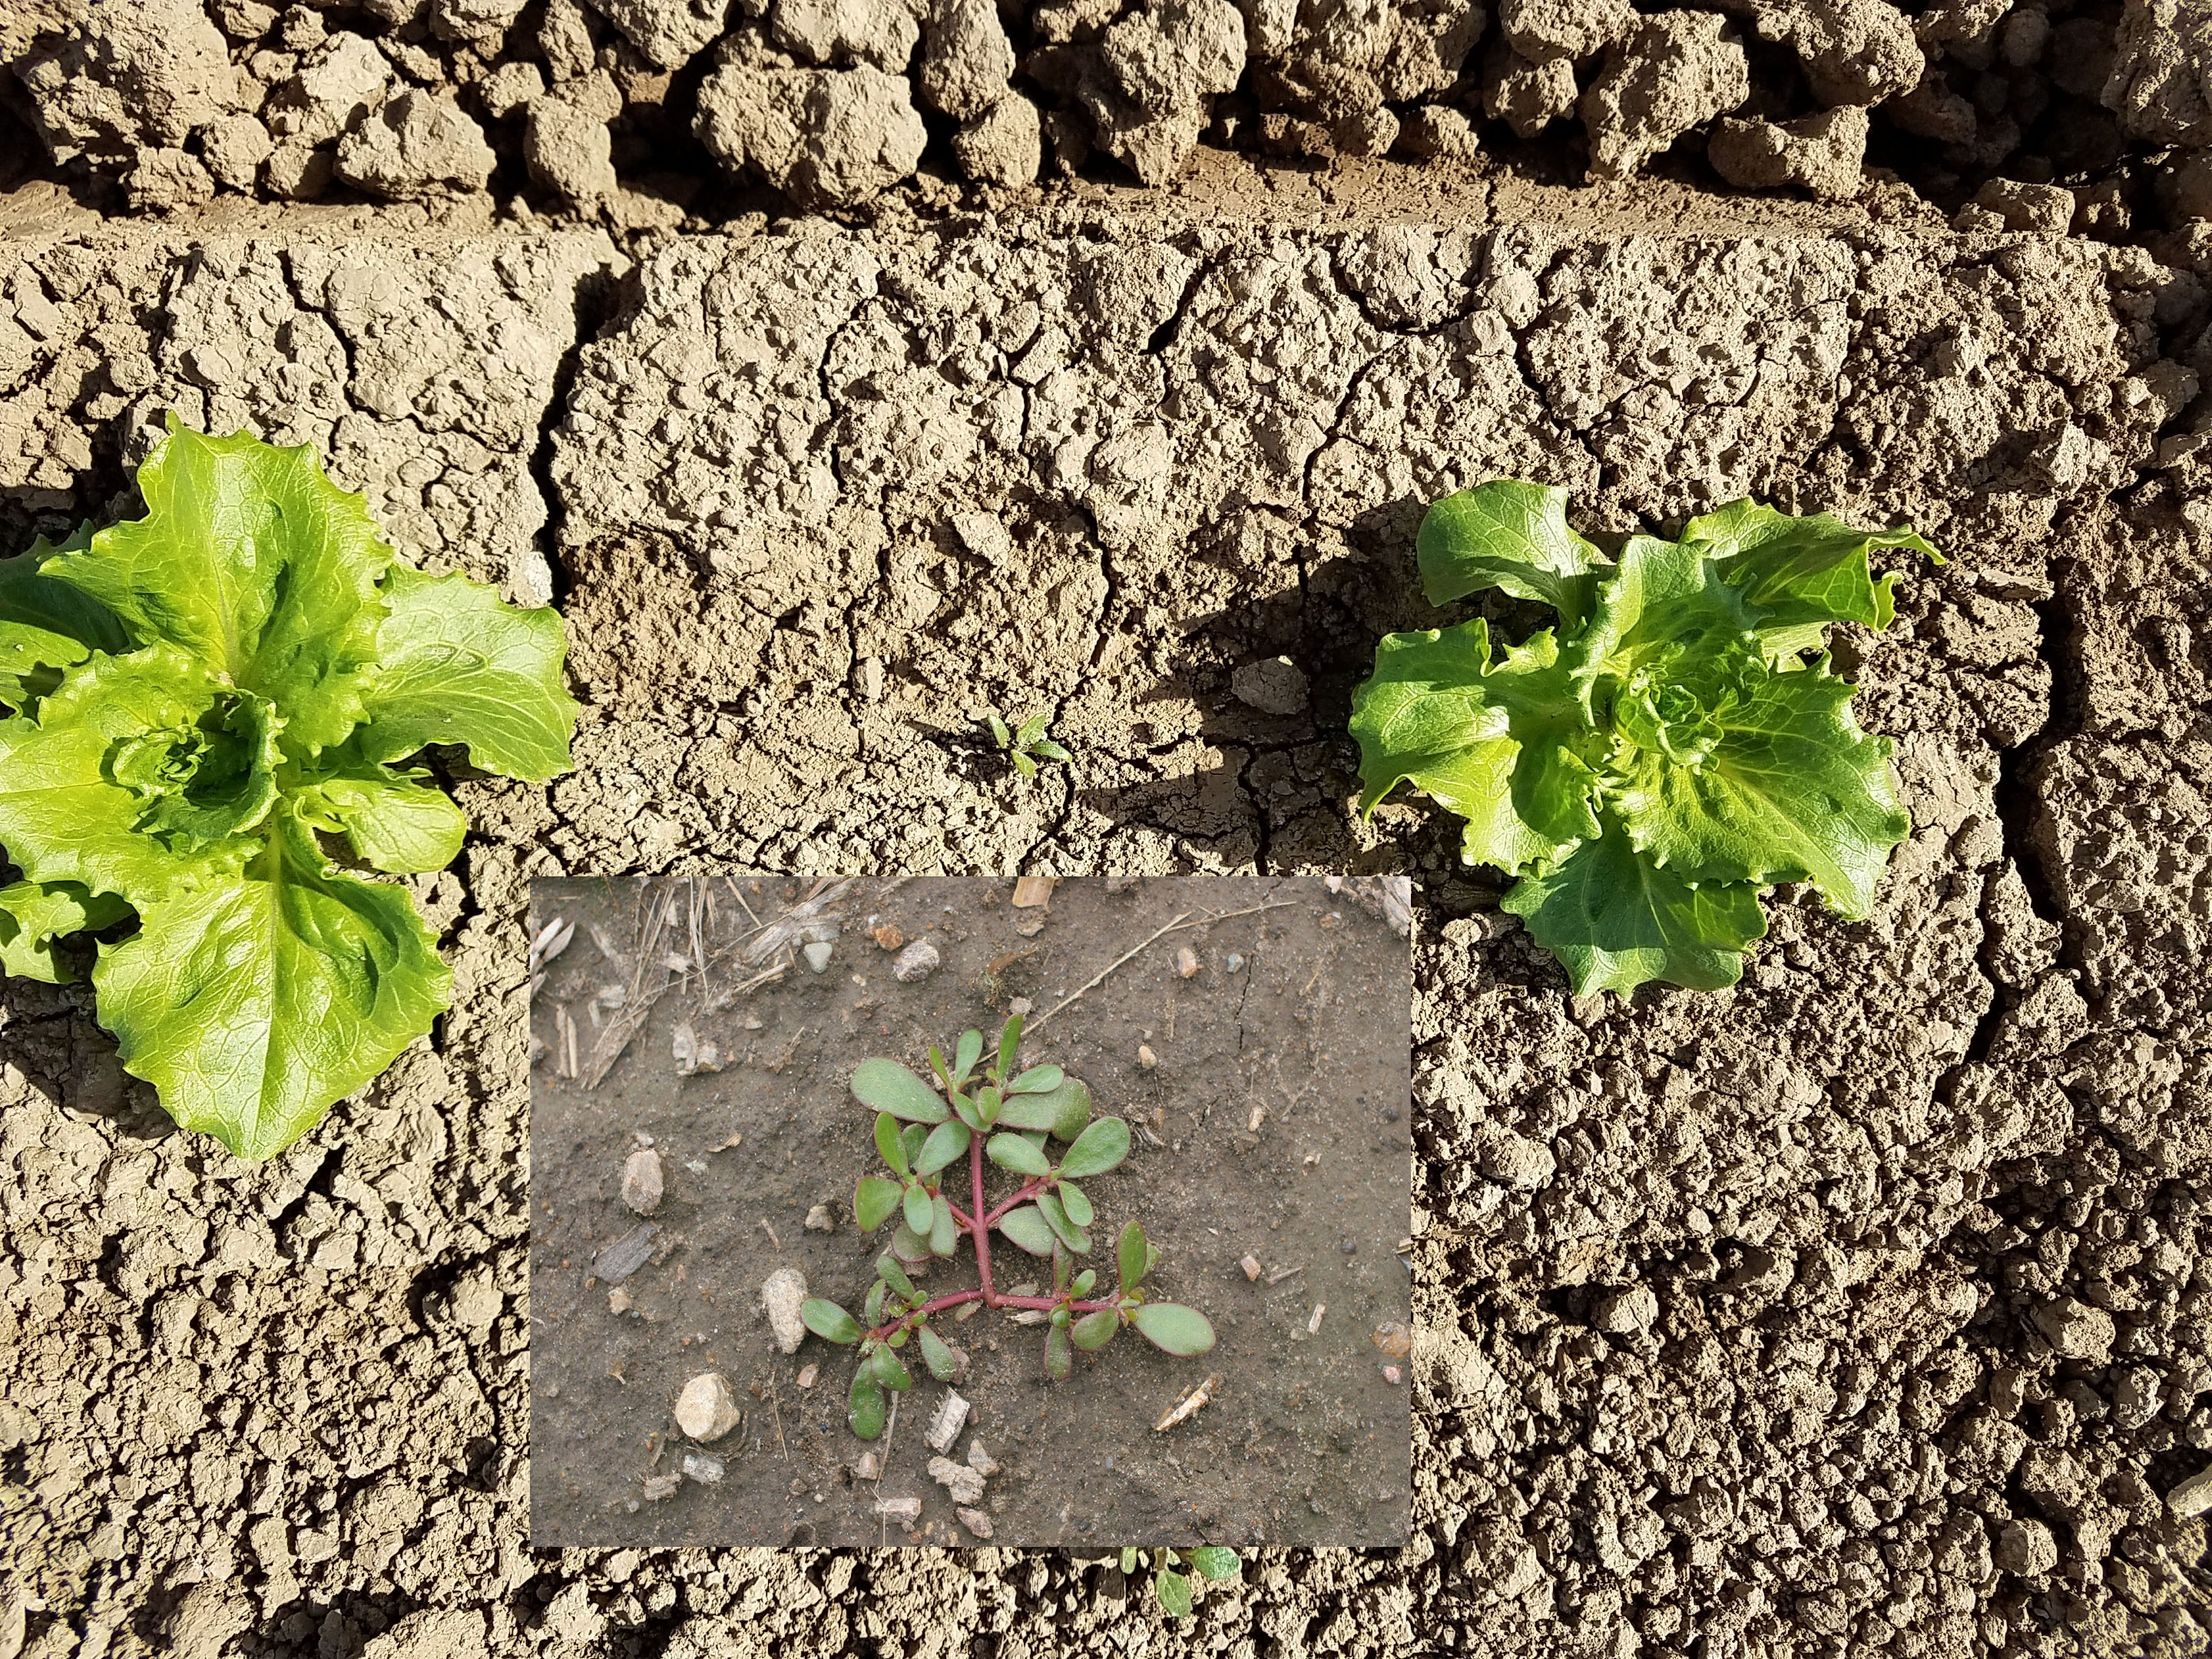
\includegraphics[width=6cm]{./figures/arranged-with-purslane-before.jpg}
%		\caption{Lettuce \& Purslane}
%		\label{fig:purslane-before}
%	\end{subfigure}
%	\begin{subfigure}[h]{.40\textwidth}
%		\centering
%		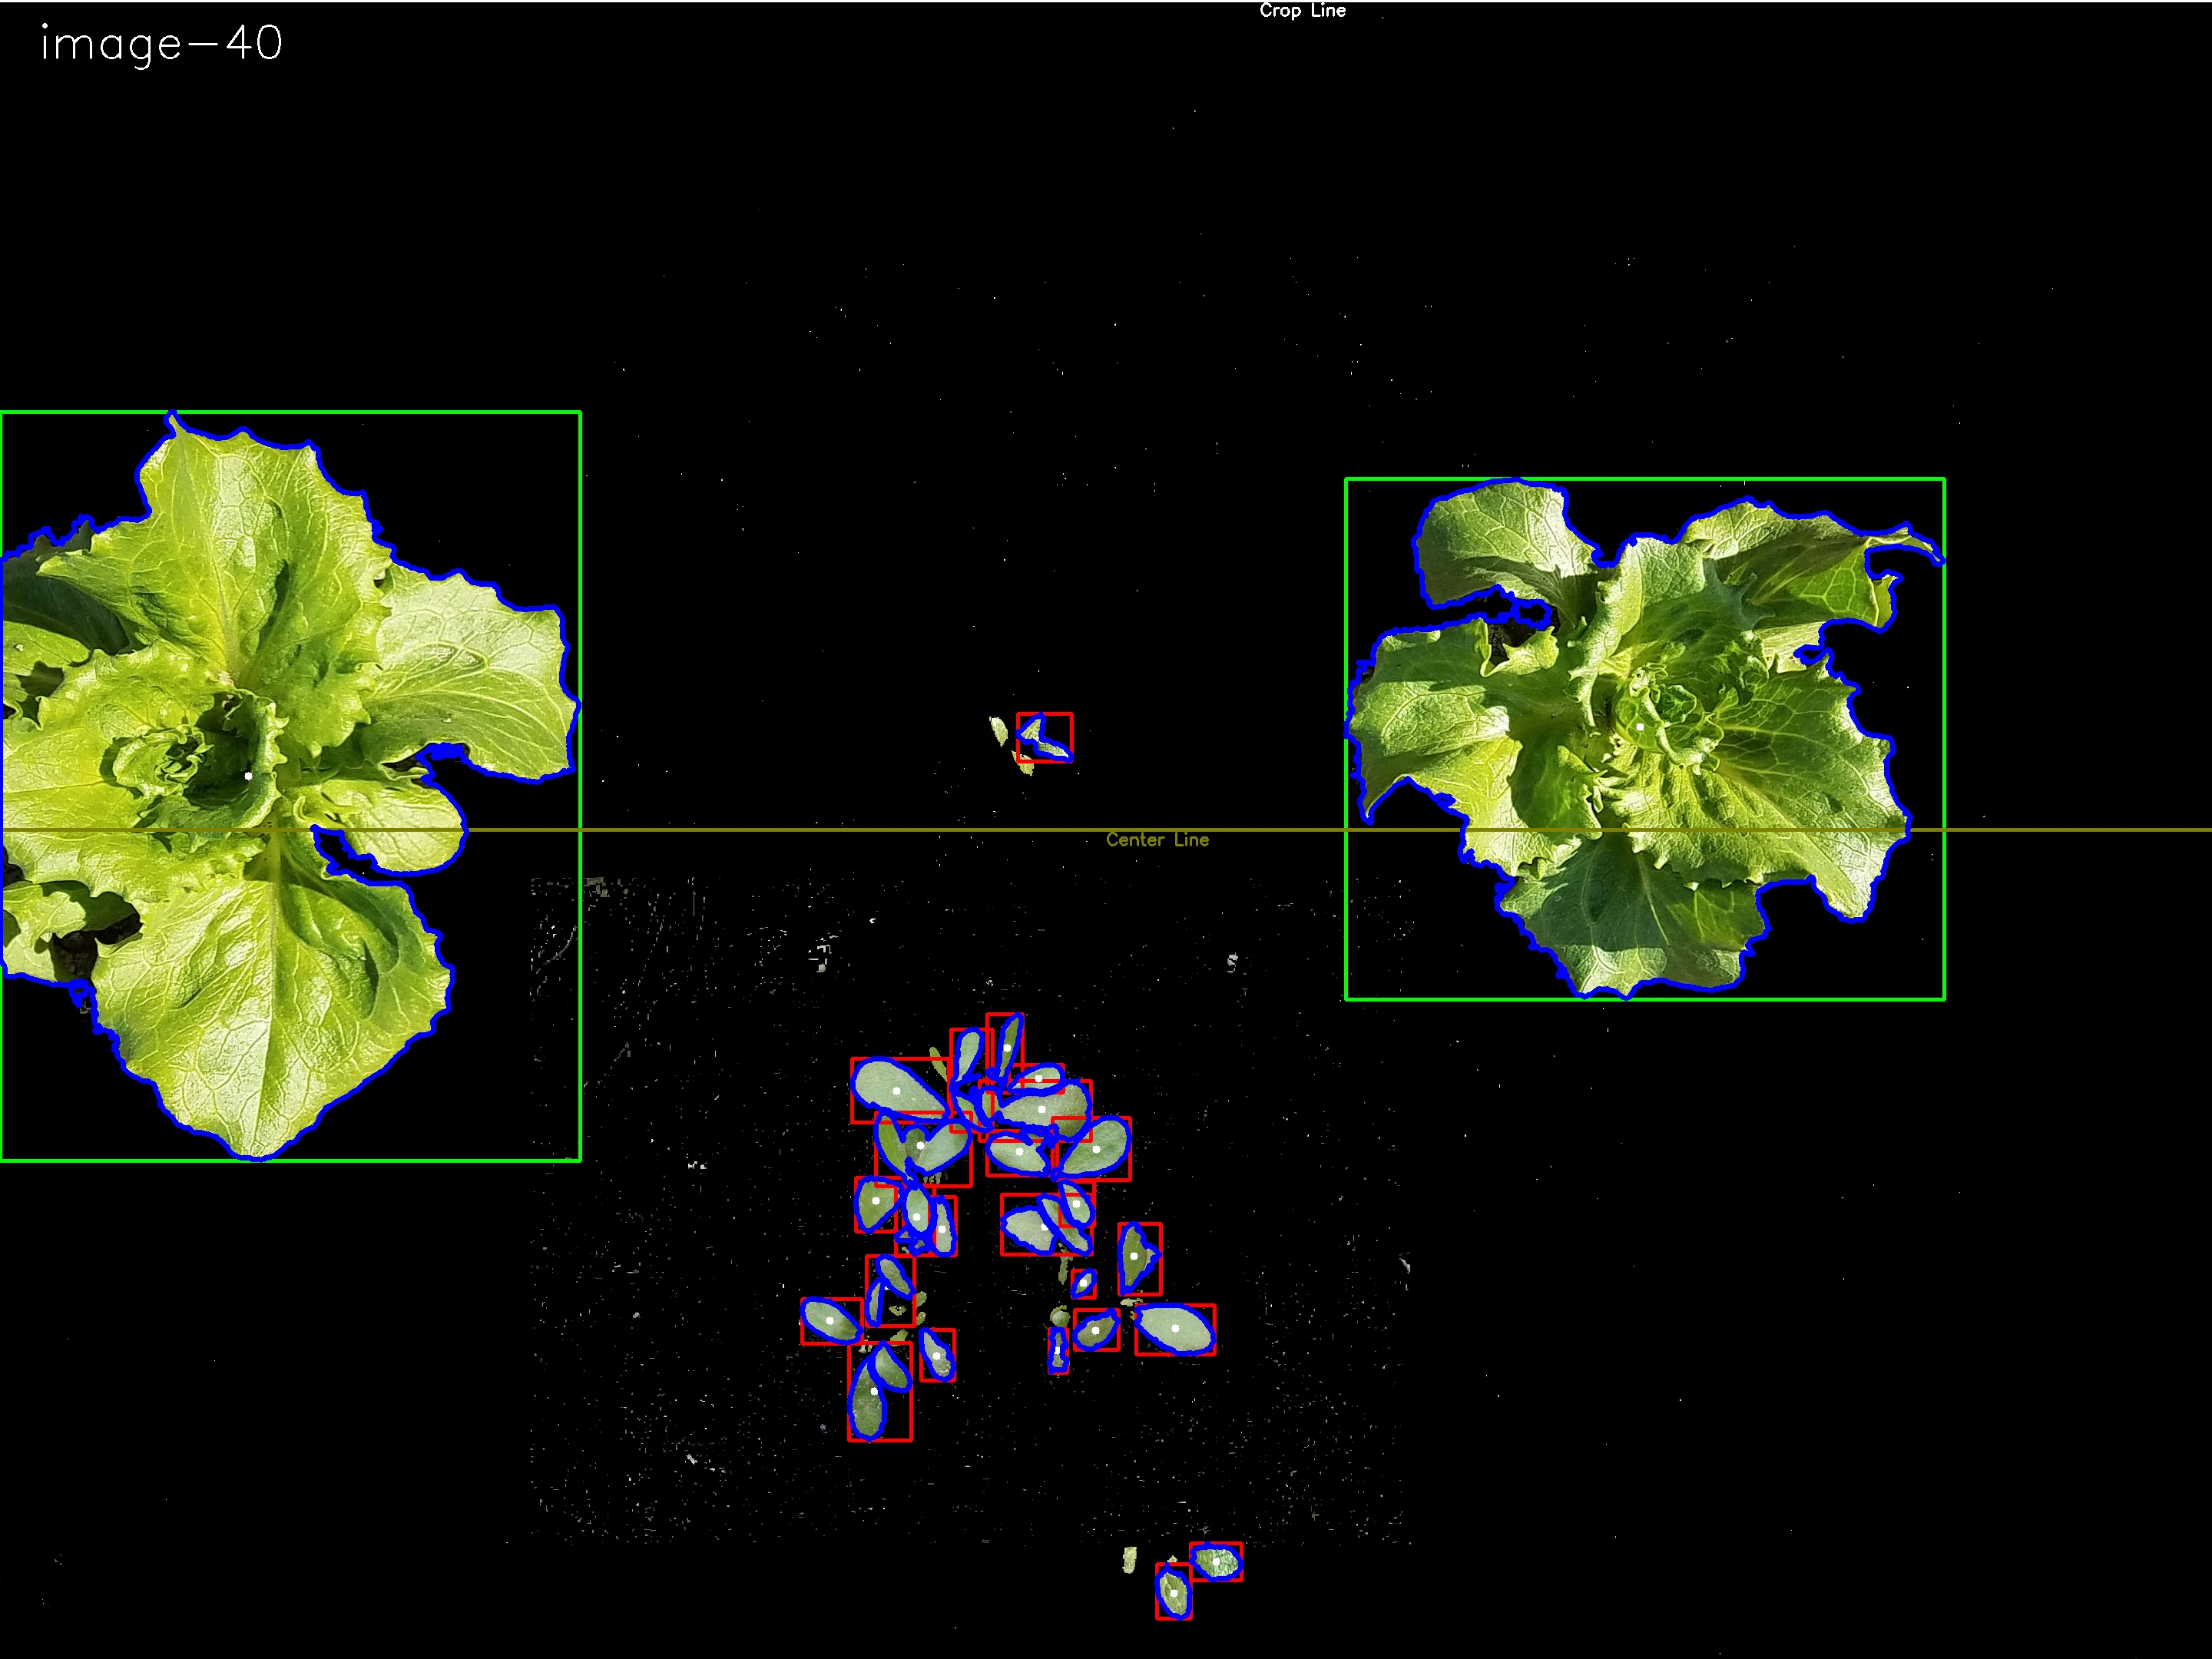
\includegraphics[width=6cm]{./figures/arranged-with-purslane-after.jpg}
%		\caption{After segmentation and classification}
%		\label{fig:purslane-after}
%	\end{subfigure}
%	\caption[Segmentation problems do not affect classification]{While the red stems of the purslane are not present in the arranged image shown here, making each leaf appear as a separate plant, this does not negatively impact the classification. (Note that the purslane image is the same one as is used in Figure~\ref{fig:purslane}). This is likely due to the relatively small contribution the stems make to GLCM calculations. While one plant is identified here as numerous individuals, each of those classifications is made correctly.}
%	\label{fig:purslane-classification}
%\end{figure}

\section{Manual Classification}
As the classification methods are supervised, producing a classified dataset is required. That is, a human must first mark up each entry in the set of identified vegetation to indicate the class (crop or weed) to which each belongs.  While the specific number of images will vary with the altitude, overlap, and ground area, the fairly small ground area imaged will result in a small set of images (the total for each collection is shown in Table \ref{tab:acquisition}), even those taken at altitudes as low as \SI{2.0}{\meter} AGL.

\begin{wraptable}{R}{5.5cm}
	\def\arraystretch{0.70}
	\caption{Image Counts}
 	\label{tab:acquisition}
 	\begin{tabular}[t]{ll} 
		\textbf{AGL} & \textbf{Images} \\
		\midrule
		      0.5m & 85  \\
		      1.0m & 65  \\
		      2.0m & 52 \\
		      5.0m & 6  \\
		      20cm & 20 
	\end{tabular}
\end{wraptable}


To allow for (relatively) painless class assignment for the images, a custom label application was developed\footnote{Development details are supplied elsewhere, but the application was developed in Python using the PyQt5 framework for GUI applications} that presented each segmented image for manual classification. Each of the blobs in the image are assigned a class by the user. That is, a human establishes the ground truth of each plant. The end result of this is to produce a training set that can be used in subsequent algorithmic classification.
\begin{figure}[H]
	\centering
	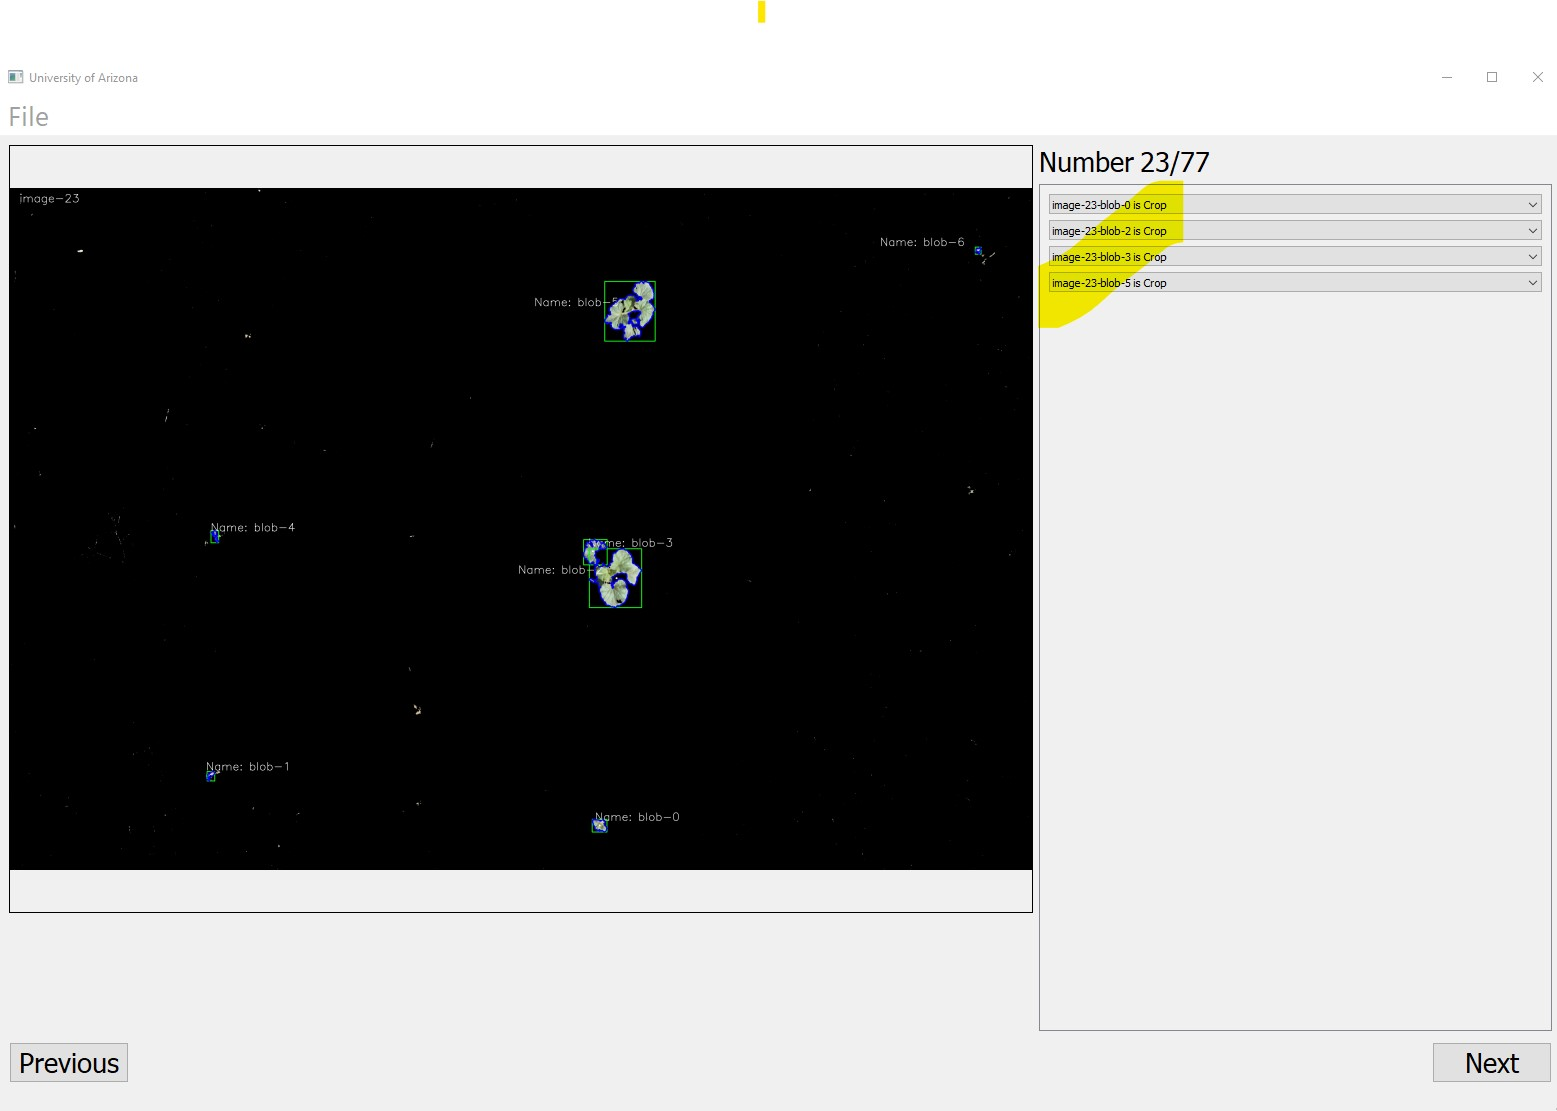
\includegraphics[scale=0.25]{./figures/screenshot-classification.jpg}
	\caption[Manual classification application screenshot]{Each blob is manually labeled with the correct class, allowing for the supervised classification approaches to classification presented later in this document to function and to assess accuracy. This application presented each image and initial assignment of the individual plants contained within that image, allowing the human expert to correct the initial assignment. Note that the initial assignment is merely for convenience -- the initial class assignment could just as well have been arbitrary.}
	\label{fig:screenshot-classification}
\end{figure}

\begin{tiny}
% Highlight the last column
\begin{longtable}{llllllh}
\caption[Vegetation Type before Manual Classification]{Vegetation Type before Manual Classification}\\
\toprule
All other & cie\_b\_contrast\_avg	 & cie\_b\_dissimilarity\_avg	& cie\_b\_ASM\_avg	& name & number & \textbf{type} \\
\midrule
\endfirsthead
\caption[]{Parameter Rankings} \\
\toprule
All other & cie\_b\_contrast\_avg	 & cie\_b\_dissimilarity\_avg	& cie\_b\_ASM\_avg	& name & number & \textbf{type} \\
\midrule
\endhead
\midrule
\multicolumn{5}{r}{{Continued on next page}} \\
\midrule
\endfoot

\bottomrule
\endlastfoot

- &6301.011981218508	&49.71044205222172	&0.4685115397070943	&image-30-blob-0	&180	&0 \\
- &4175.090715594958	&41.10014962780084	&0.1362153347621408	&image-30-blob-1	&181	&0 \\
- &6156.428566816558	&49.36721780237519	&0.4390896935316736	&image-30-blob-2	&182	&0 \\
- &2488.164269406393	&29.97195585996956	&0.046253458	           &image-30-blob-3	&183	&0 \\
- &4975.8718916524285	&45.74685146509714	&0.2129808994576038 &image-30-blob-6	&186	&0 \\
- &3515.707728494623	&43.87426075268817	&0.028970925	           &image-30-blob-7	&187	&0
\end{longtable}
\end{tiny}

%
% I M B A L A N C E
%
\section{Class Imbalance}
Plantings often exhibit a somewhat inconvenient feature: weeds and crop do not appear in the same proportion. While having a low weed count is probably desirable for crop production, it is While this can present itself as a relatively mild imbalance of nine weed plants for every 10 crop plants or a more extreme ratio of 1000 crop plants for every weed. \citeauthor{Fernandez2018-fw}, in a book discussing imbalanced datasets, detail several correction algorithms, among them SMOTE, ADASYN, Borderline SMOTE, kmeans, and SVM \parencite{Fernandez2018-fw}. While the imbalance ratio of the training set will most assuredly deviate from the 1:1 ideal, it is not particularly important what the specific ratio is, as the data will be trimmed to reflect the various ratios. That is, while a dataset may have a relatively low imbalance of 10:8, samples of the minority class are discarded to achieve a much higher imbalance. As Figure \ref{fig:imbalance} shows, substituting synthetic data improves the F1 scores of various classification techniques in most cases, but some of the impact is quite trivial and -- in rare cases -- detrimental (note the case of using a \textit{kmeans} approach to correct the data for a \textit{decision tree} classification). In most cases. of course, the solution 
\begin{figure}[H]
	\centering
	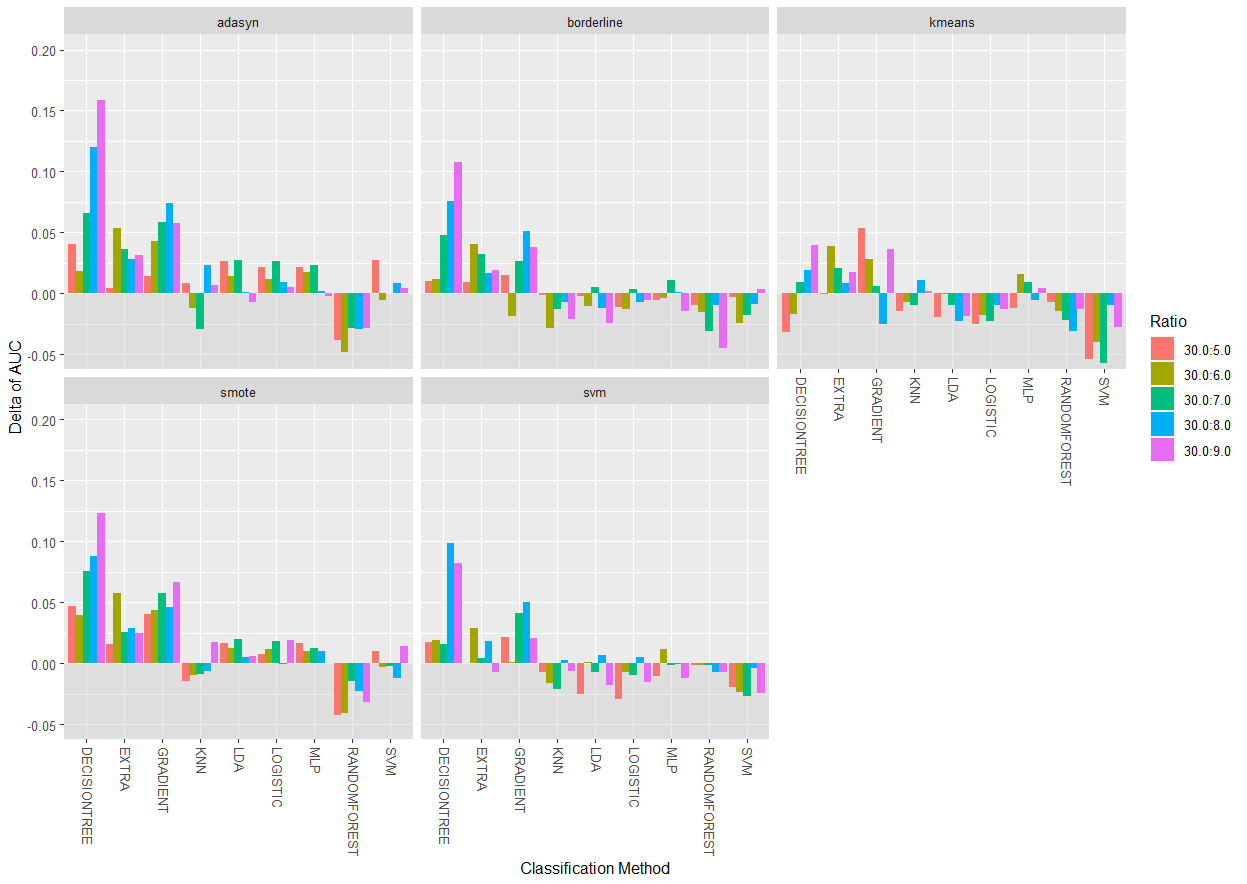
\includegraphics[width=0.9\linewidth]{./figures/imbalance.png}
	\caption[Class imbalance correction techniques]{The impact on F1 scores of class imbalance correction techniques for various ratios and classification strategies can be seen in this visualization. The F1 score of the multi-layer perceptron classification, for instance, starting with a dataset with a 30:2 imbalance, is increased by 85\% when the imbalance is corrected using the ADASYN algorithm.}
	\label{fig:imbalance}
\end{figure}
%
% S Y S T E M  D E S I G N
%
\section{System Design}
\subsection{Database}
The database held two collections\footnote{The database selected for this project is a document-oriented database, MongoDB. While a detailed discussion of a document-oriented database is beyond the scope of this document, an overly simple comparison to the more frequently encountered relational (SQL) database is to consider collections to be a bit like tables in that model.}, \textit{images} and \textit{blobs}.

The \textit{images} collection held records relating to each of the images gathered:
\begin{itemize}
	\item{\textit{Latitude}, the geographic latitude where the image was acquired}
	\item{\textit{Longitude}, the geographic longitude where the image was acquired}
	\item{\textit{AGL}, the distance above the ground where the image was acquired}
	\item{\textit{Crop}, the crop in the image}
	\item{\textit{Date acquired}, the date the image was acquired}
	\item{\textit{Segmentation Results}, the resulting image of various segmentation algorithms given in Table~\ref{tab:segmentation-formulae}}	
	\item{\textit{Processing Results}, the resulting image of various learning approaches}	
	\item{\textit{Hash}, an identifier of the image}	
\end{itemize}
 While the collection holds resulting images, the database holds only information about the resulting image, not the image itself. The image itself is too large to efficiently store in the database, and is stored in a file on disk. While most of the remaining attributes are widely familiar (and many are directly abstracted from the image EXIF data), the notion of an image \textit{hash} warrants mention here. The hash of an image is the unique fingerprint of the image's bits. This allows the software to definitively determine if a specific image is already within the database. This assessment, however, is not without an important caveat: any modification -- even to an image's EXIF metadata -- will result in an image that will be considered distinct to an otherwise nearly identical image. As image records are inserted into the database only after pre-processing steps -- such as color correction-- are complete, this caveat will ordinarily not affect operation.
 
 The \textit{blobs} collection held records relating to each plants:
 \begin{itemize}
 	\item{\textit{Factors}, the color, shape, and texture factors detailed in prior sections}	
	\item{\textit{Classification}, the predicted class of the blob}	
	\item{\textit{Actual}, the actual class of the blob}	
	\item{\textit{Machine Learning Approach}, the machine learning approach used}	
	\item{\textit{Factors Used}, the factors used for classification}	
	\item{\textit{Parent}, the image in which this blob is found}
	\item{\textit{Hash}, an identifier of the blob}	
 \end{itemize}

There is a 1:N relationship between an image and the blobs found within that image, but the relationship is actually between the segmented image and the blobs found within that segmented image, as the size of the blob will vary based on the segmentation approach.

% 
% I M A G E  A C Q U I S I T I O N
%
\section{Acquisition of Images in Study Area and Processing}
Image acquisitions were carried out at the Maricopa Agricultural Center (MAC) on a cantaloupe planting (N 33.061857, E 111.967145) consisting of 3 water treatments: flood, drip, and center-pivot, each watered at 80\% and 100\%. Only the flood treatment will be imaged and considered for this study. This is mostly motivated by practical considerations: it is not anticipated that the drip treatment plots will have a significant number of weeds, and while avoiding the center-pivot device during UAV flights at low altitudes is not particularly difficult, images will not be collected in that part of the field.  Image acquisition will take place on at regular intervals beginning in April 2024 and continuing through May 2024. All images were acquired using a DJI Mavic Air 2S with a stock RGB 20 MP sensor. The UAV camera has the following relevant details:

\begin{itemize}
	\item{13.25mm sensor width}
	\item{8.38mm focal length}
	\item{5464 pixel width}
	\item{3640 pixel height}
\end{itemize}

Missions were planned and executed with Dronelink software, a commercially available package.  Where feasible, missions were conducted in the same ambient light conditions, but an exact match of ambient conditions using uncontrolled lighting is not always possible.
As illustrated by Figure \ref{fig:field-layout} the largest flood irrigated area is \SI{4536}{\metre\squared}, a location where image acquisition took place. While images of this reduced subset will reduce the presence of plants in the adjacent drip irrigation plots, this will not ensure that they are not imaged.  Consider the size of the ground captured with a UAV flight at various heights:

\begin{table*}[h!] \centering
\begin{tabular}{SSSSSSSS} \toprule
    {AGL (m)} & {Captured Width (m)} & {Images} \\ \midrule
    1  & 2 & xxx \\
    2  & 3  & xxx  \\
    5  & 8  & xxx  \\
    10  &16  & xxx     \\
    20 &32 & xxx \\ \bottomrule
\end{tabular}
\caption{Ground captured at various distances AGL}
\label{table:captured}
\end{table*}
As Table \ref{table:captured} shows, the capture area is approaching the width of three plots at 10 meters AGL and exceeding the flood treatment area and 20 meters AGL. While capturing images in the adjacent plots was undesired, doing so had no appreciable affects in classification.

\begin{figure}[h!]
	\centering
	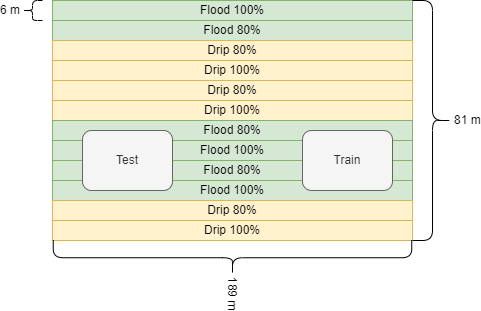
\includegraphics[width=0.8\linewidth]{./figures/test-area.png}
	\caption[Field layout for image acquisition]{The train and test subsets of the 80\% and 100\% water treatment of the flood irrigation is considered for this study. As the drip irrigation is not likely to show many weeds, it was not considered for this study.}
	\label{fig:field-layout}
\end{figure}

Images were color corrected against images taken before each flight of a Spyder CHECKR24 calibration target. The digital negative of each image (DNG, a standard format for raw sensor data) was corrected and converted to JPG format for subsequent processing.\footnote{The merits of raw, uncompressed, and unprocessed sensor data versus compressed, processed formats like JPG are beyond the scope of this document, but it is fair to say taking raw sensor data, processing, and then producing a compressed JPG is precisely what consumer products like phone cameras do. So that the color correction step can be inserted, the process of producing an image that can be viewed with most software is altered a bit, but essentially unchanged.}

As illustrated in Figure \ref{fig:field-layout}, the train and test image sets acquired were physically separate. The goal is simple to state: items in the training subset should never appear in the testing subset. The side-lap and front-lap of UAV acquired images makes this task much more difficult, although any set of images of adjacent objects will exhibit this complication. Consider a UAV image acquisition of three plants, as shown in Figure \ref{fig:uav-overlap}. In this example, plants (even if it is only a portion) appear in multiple images. While this is expected -- and even desired for stitching the images together -- this complicates splitting the image set into train and test segments such that the same plant does not appear in both segments. The most pragmatic approach here is to simply avoid the problem by not performing a split at all. Collecting, instead, a completely separate train and test set of images. This approach has an additional benefit in that a test set can now be acquired from a different part of the field. Consider the case where the test set is taken from the \textit{drip} treatment area. While it will not have a particularly high weed load, it should be possible to classify the crop in that image set with the same accuracy as seen in the image set taken in the \textit{flood} treatment. While this study did not examine classification accuracy across water treatment methods, the clean separation of the train and test segments also means that test segments can be captured for different crops or different portions of the same field.

\begin{figure}[h!]
	\centering
	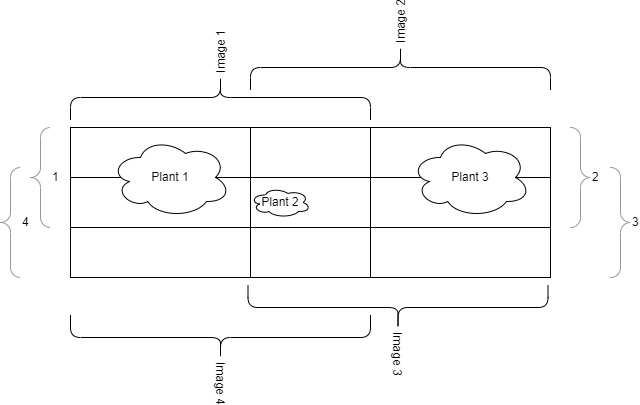
\includegraphics[width=0.5\linewidth]{./figures/overlap.png}
	\caption[Image overlap in UAV images]{The same plant appears in multiple images. As seen here, plants \#1 and \#3 appear in two (fully in images \#1 and \#2, partially in images \#3 and \#4), and plant \#3 appears in full in four images. A train/test split is possible, of course, but requires knowledge of what an image contains.}
	\label{fig:uav-overlap}
\end{figure}

	
%
% L A B E L S
%
\section{Manual Classification}
Each image was manually classified using a Python application that took the initial results of the image segmentation, blob identification, and classification to allow the user to assign the correct assignment for each plant. This process was not to part of the process to provide an accuracy score, but to label each blob with the true classification to be used in the supervised approach discussed in subsequent sections. As individual plants are not geo-located -- and assignments could not simply be made once for a location and then applied to all image sets -- it was necessary to perform this manual step for each image acquired at each altitude, as the exact position of a specific plant differed in each image set.

\begin{figure}[h!]
	\centering
	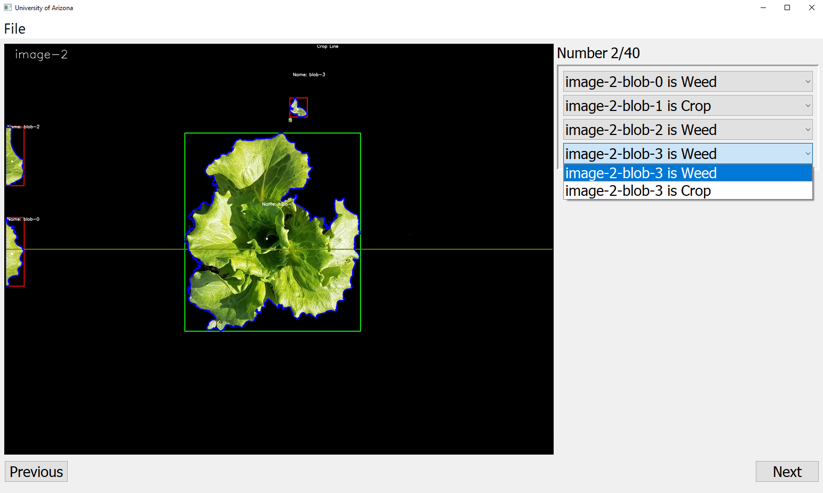
\includegraphics[width=12cm]{./figures/label-screenshot.png}
	\label{fig:label-screenshot}
	\caption[Screenshot of application for manually labeling blobs]{Each blob is manually labeled with the correct class, allowing for the supervised classification approaches to classification presented later in this document to function and to assess accuracy. This application presented each image and initial assignment of the individual plants contained within that image, allowing the human expert to correct the initial assignment. Note that the initial assignment is merely for convenience -- the initial class assignment could just as well have been arbitrary.}
\end{figure}


\section{Feature Selection}
The features described in the previous section were generated for a set of segmented images, resulting in each plant being described by 715 attributes. Several techniques were then used to explore the relationship between these attributes and the labeled class: Recursive Feature Elimination, Principle Component Analysis (PCA), Feature Importance, and Univariate feature selection.  Specifically, only the most important variables will be selected in the predictions, and those parameters with a weak association are dropped. Unfortunately, different feature ranking techniques identified sets of the most significant features without a clear overlap. There were exceptions to this, of course, as can be seen with the feature \textit{saturation\_mean} identified with the highest rank in most of the analysis.
While the features shown in Table~\ref{table:parameters} are not completely consistent with each other there are a few themes:
\begin{itemize}
\item{Aspects of color data are quite predictive, particularly the saturation of the color.}
\item{Most structural attributes (convexity, roundness, etc) are not significant.}
\item{Statistical analysis of the gradients and pixels relationship to each other is significant.}
\end{itemize}

Of these initial findings, it was somewhat unexpected that shape parameters were not among the most significant features.

%
% Begin Copy-Paste
%

\begin{longtable}{lllll}
\caption[Parameter Rankings]{Parameter Rankings}\\
\toprule
{} &               Recursive &              PCA &              Importance &                 Univariate \\
\midrule
\endfirsthead
\caption[]{Parameter Rankings} \\
\toprule
{} &               Recursive &              PCA &              Importance &                 Univariate \\
\midrule
\endhead
\midrule
\multicolumn{5}{r}{{Continued on next page}} \\
\midrule
\endfoot

\bottomrule
\endlastfoot
0 &                in\_phase &              hue &  greyscale\_contrast\_avg &      green\_correlation\_avg \\
1 &    ycbcr\_y\_contrast\_avg &  saturation\_mean &                hog\_mean &               hog\_variance \\
2 &    blue\_correlation\_avg &         in\_phase &                in\_phase &  ycbcr\_y\_dissimilarity\_avg \\
3 &  greyscale\_contrast\_avg &          cb\_mean &    greyscale\_energy\_avg &    hsv\_hue\_homogeneity\_avg \\
\end{longtable}

% End Copy-Paste
 To clarify the names of the parameters
 \begin{itemize}
 	\item{\textit{in\_phase} -- the in-phase component of the YIQ colorspace}
 	\item{\textit{ycbcr\_y\_contrast\_avg} -- the mean of the contrast GLCM computation of the $Y$ component of the YCbCr colorspace}
 \end{itemize}
 	

The set of unique parameters across the top 10 selection techniques was relatively small, yielding a search space of 348,330,136 combinations. This parameter space was exhaustively searched to find the set of parameters best suited for each of the  seven classification techniques:
\begin{itemize}
	\item{Random Forest (Abbreviated to RF in sections of this document)}
	\item{K Nearest Neighbors (KNN)}
	\item{Gradient Boosting (GRADIENT}
	\item{Logistic Regression (LR)}
	\item{Decision Tree (DT)}
	\item{Support Vector Machine (SVM)}
	\item{Linear Discriminate Analysis (LDA)}
	\item{Multi-layer Perceptron (MLP)}
	\item{Extra Trees (Extra)}
\end{itemize}

As there was no clear agreement between the parameters identified by the selection mechanisms, the results were analyzed to assess the outcome of using a given selection technique and how similar 
\footnote{The similarity between two lists is given here by the \textit{cosine similarity}, a technique that considers the elements of an array as vectors in n-dimensional space. In this case, there is a bit of pre-processing of the data, as a list of factors is not something that directly lends itself to computation analysis. Instead, the arrays are converted to lists of the frequency of each term. While this may sound uninteresting at first glance, this information can be used to determine how similar two lists are. The formula $\frac {(A \cdot B)} { \lVert A \rVert * \lVert B \rVert }$ is used to produce that metric.}
the parameters selected by that technique were to the ones identified by other techniques. 

\subsection{Texture}
\subsection{Color}
\subsection{Shape}
\subsection{Optimal}

In Table \ref{table:matches-selection}, Decision Tree classification, for instance, shows a 98\% accuracy with the parameter set identified by \textit{PCA}, but that parameter set is only 25\% similar to the one identified by \textit{Recursive Feature Elimination}. Of special note here is \textit{Feature Importance}. Top accuracy results never matched any of the parameters identified with that technique -- thus the similarity scores of 0 in the table.

\begin{tiny}
% Begin copied table from the output of this command and slightly modified
%  python results.py -p reviewed -s 1.0 -c parameters.pickle -o show

\begin{longtable}{lcrrrr}
\caption[short caption]{Parameter selection techniques}
\label{table:matches-selection}\\
\toprule
% Begin edits
& & \multicolumn{4}{c}{Similarity to Parameters Found}\\
\cmidrule{3-6} 
\multicolumn{1}{c}{Classification} & \multicolumn{1}{c}{AUC} & \multicolumn{1}{c}{Recursive} &  \multicolumn{1}{c}{PCA} & \multicolumn{1}{c}{Importance} & \multicolumn{1}{c}{Univariate} \\
% End edits
\midrule
\endfirsthead
\caption[]{Parameter selection techniques} \\
\toprule
% Begin edits
& & \multicolumn{4}{c}{Similarity to Parameters Found}\\
\cmidrule{3-6} 
\multicolumn{1}{c}{Classification} & \multicolumn{1}{c}{AUC} & \multicolumn{1}{c}{Recursive} &  \multicolumn{1}{c}{PCA} & \multicolumn{1}{c}{Importance} & \multicolumn{1}{c}{Univariate} \\
% End edits
\midrule
\endhead
\midrule
\multicolumn{6}{r}{{Continued on next page}} \\
\midrule
\endfoot

\bottomrule
\endlastfoot
DECISIONTREE & 0.98 &      0.25 & 1.00 &       0.00 &       0.50 \\
DECISIONTREE & 0.96 &      0.25 & 0.50 &       0.00 &       1.00 \\
DECISIONTREE & 0.97 &      1.00 & 0.25 &       0.00 &       0.25 \\
       EXTRA & 0.97 &      0.25 & 1.00 &       0.00 &       0.50 \\
       EXTRA & 0.96 &      0.25 & 0.50 &       0.00 &       1.00 \\
       EXTRA & 0.96 &      1.00 & 0.25 &       0.00 &       0.25 \\
    GRADIENT & 0.98 &      0.25 & 1.00 &       0.00 &       0.50 \\
    GRADIENT & 0.96 &      0.25 & 0.50 &       0.00 &       1.00 \\
    GRADIENT & 0.97 &      1.00 & 0.25 &       0.00 &       0.25 \\
         KNN & 0.96 &      0.25 & 1.00 &       0.00 &       0.50 \\
         KNN & 0.96 &      0.25 & 0.50 &       0.00 &       1.00 \\
         KNN & 0.96 &      1.00 & 0.25 &       0.00 &       0.25 \\
         LDA & 0.97 &      0.25 & 1.00 &       0.00 &       0.50 \\
         LDA & 0.98 &      0.25 & 0.50 &       0.00 &       1.00 \\
         LDA & 0.96 &      1.00 & 0.25 &       0.00 &       0.25 \\
    LOGISTIC & 0.96 &      0.25 & 1.00 &       0.00 &       0.50 \\
    LOGISTIC & 0.96 &      0.25 & 0.50 &       0.00 &       1.00 \\
    LOGISTIC & 0.85 &      1.00 & 0.25 &       0.00 &       0.25 \\
         MLP & 0.98 &      0.25 & 1.00 &       0.00 &       0.50 \\
         MLP & 0.97 &      0.25 & 0.50 &       0.00 &       1.00 \\
         MLP & 0.96 &      1.00 & 0.25 &       0.00 &       0.25 \\
RANDOMFOREST & 0.99 &      0.25 & 1.00 &       0.00 &       0.50 \\
RANDOMFOREST & 0.98 &      0.25 & 0.50 &       0.00 &       1.00 \\
RANDOMFOREST & 0.96 &      1.00 & 0.25 &       0.00 &       0.25 \\
         SVM & 0.95 &      0.25 & 1.00 &       0.00 &       0.50 \\
         SVM & 0.96 &      0.25 & 0.50 &       0.00 &       1.00 \\
         SVM & 0.78 &      1.00 & 0.25 &       0.00 &       0.25 \\



\end{longtable}


%Endcopiedtable
\end{tiny}
Table~\ref{table:optimal-auc} contains the result of this search with the accuracy scores using an average across 5 folds.

\begin{tiny}
% -- begin copied table
\begin{longtable}{lllllllll}
\caption[Optimal Parameters for AUC]{Optimal Parameters by Technique (AUC)}
\label{table:optimal-auc}\\
\toprule
RANDOMFOREST &             KNN &        GRADIENT &         LOGISTIC &       DECISIONTREE &             SVM &
        LDA &                             MLP &            EXTRA \\
\midrule
\endfirsthead
\caption[]{Optimal Parameters by Technique (AUC)} \\
\toprule
RANDOMFOREST &             KNN &        GRADIENT &         LOGISTIC &       DECISIONTREE &             SVM &
        LDA &                             MLP &            EXTRA \\
\midrule
\endhead
\midrule
\multicolumn{9}{r}{{Continued on next page}} \\
\midrule
\endfoot

\bottomrule
\endlastfoot
0.986736 &         0.99875 &        0.982639 &         0.999167 &           0.998889 &        0.998472 &
    0.99875 &                        0.999722 &         0.999167 \\
cie\_b\_ASM\_avg &         cb\_mean &   cie\_b\_ASM\_avg &       hog\_stddev &         hog\_stddev &         cb\_mean &
        cie\_b\_ASM\_avg &                   cie\_b\_ASM\_avg &          cb\_mean \\
hsi\_intensity\_dissimilarity\_avg &   cie\_b\_ASM\_avg &      hog\_stddev &         in\_phase &           in\_phase &      hog\_stddev & hsi\_inten
sity\_dissimilarity\_avg & hsi\_intensity\_dissimilarity\_avg &    cie\_b\_ASM\_avg \\
hue &      hog\_stddev &             hue &  saturation\_mean &    saturation\_mean &             hue &                 s
aturation\_mean &                             hue &  saturation\_mean \\
saturation\_mean & saturation\_mean & saturation\_mean & ycbcr\_cr\_ASM\_avg & yiq\_q\_contrast\_avg & saturation\_mean &
     yiq\_q\_energy\_avg &                 saturation\_mean & yiq\_q\_energy\_avg \\
\end{longtable}


% -- end copied table
\end{tiny}

% TEMPORARY

% Begin Drip/Pivot
%
\begin{tiny}
% Begin copied table
\begin{longtable}{lrrrrr}
\caption[Parameter selection similarities]{Parameter selection similarities for Drip/Pivot}
\label{table:matches-selection}\\
\toprule
% Begin edits
& & \multicolumn{4}{c}{Similarity to Parameters Found}\\
\cmidrule{3-6} 
\multicolumn{1}{c}{Technique} & \multicolumn{1}{c}{Accuracy} & \multicolumn{1}{c}{Recursive} &  \multicolumn{1}{c}{PCA} & \multicolumn{1}{c}{Importance} & \multicolumn{1}{c}{Univariate} \\
% End edits
\midrule
\endfirsthead
\caption[]{long caption} \\
\toprule
% Begin edits
& & \multicolumn{2}{c}{Similarity to Parameters Found}\\
\cmidrule{3-6} 
\multicolumn{1}{c}{Technique} & \multicolumn{1}{c}{Accuracy} & \multicolumn{1}{c}{Recursive} &  \multicolumn{1}{c}{PCA} & \multicolumn{1}{c}{Importance} & \multicolumn{1}{c}{Univariate} \\
% End edits
\midrule
\endhead
\midrule
\multicolumn{6}{r}{{Continued on next page}} \\
\midrule
\endfoot

\bottomrule
\endlastfoot
DECISIONTREE & 0.69 &      0.00 & 1.00 &       0.00 &       0.00 \\
EXTRA & 0.66 &      0.00 & 1.00 &       0.00 &       0.00 \\
GRADIENT & 0.67 &      0.00 & 1.00 &       0.00 &       0.00 \\
KNN & 0.64 &      0.00 & 1.00 &       0.00 &       0.00 \\
LDA & 0.65 &      0.00 & 1.00 &       0.00 &       0.00 \\
LOGISTIC & 0.67 &      0.00 & 1.00 &       0.00 &       0.00 \\
MLP & 0.71 &      0.00 & 1.00 &       0.00 &       0.00 \\
RANDOMFOREST & 0.68 &      0.00 & 1.00 &       0.00 &       0.00 \\
SVM & 0.69 &      0.00 & 1.00 &       0.00 &       0.00 \\
\end{longtable}
\end{tiny}

%
% End Drip/Pivot


\begin{tiny}
% Begin copied table
\begin{longtable}{lrrrrr}
\caption[Parameter selection similarities]{Parameter selection similarities}
\label{table:matches-selection}\\
\toprule
% Begin edits
& & \multicolumn{4}{c}{Similarity to Parameters Found}\\
\cmidrule{3-6} 
\multicolumn{1}{c}{Technique} & \multicolumn{1}{c}{Accuracy} & \multicolumn{1}{c}{Recursive} &  \multicolumn{1}{c}{PCA} & \multicolumn{1}{c}{Importance} & \multicolumn{1}{c}{Univariate} \\
% End edits
\midrule
\endfirsthead
\caption[]{long caption} \\
\toprule
% Begin edits
& & \multicolumn{2}{c}{Similarity to Parameters Found}\\
\cmidrule{3-6} 
\multicolumn{1}{c}{Technique} & \multicolumn{1}{c}{Accuracy} & \multicolumn{1}{c}{Recursive} &  \multicolumn{1}{c}{PCA} & \multicolumn{1}{c}{Importance} & \multicolumn{1}{c}{Univariate} \\
% End edits
\midrule
\endhead
\midrule
\multicolumn{6}{r}{{Continued on next page}} \\
\midrule
\endfoot

\bottomrule
\endlastfoot
DECISIONTREE & 0.979454 &      0.25 & 1.00 &        0.0 &       0.50 \\
DECISIONTREE & 0.964706 &      0.25 & 0.50 &        0.0 &       1.00 \\
DECISIONTREE & 0.967690 &      1.00 & 0.25 &        0.0 &       0.25 \\
GRADIENT & 0.982353 &      0.25 & 1.00 &        0.0 &       0.50 \\
GRADIENT & 0.955925 &      0.25 & 0.50 &        0.0 &       1.00 \\
GRADIENT & 0.967690 &      1.00 & 0.25 &        0.0 &       0.25 \\
KNN & 0.955968 &      0.25 & 1.00 &        0.0 &       0.50 \\
KNN & 0.958866 &      0.25 & 0.50 &        0.0 &       1.00 \\
KNN & 0.958866 &      1.00 & 0.25 &        0.0 &       0.25 \\
LDA & 0.970631 &      0.25 & 1.00 &        0.0 &       0.50 \\
LDA & 0.976471 &      0.25 & 0.50 &        0.0 &       1.00 \\
LDA & 0.955968 &      1.00 & 0.25 &        0.0 &       0.25 \\
LOGISTIC & 0.961807 &      0.25 & 1.00 &        0.0 &       0.50 \\
LOGISTIC & 0.955968 &      0.25 & 0.50 &        0.0 &       1.00 \\
LOGISTIC & 0.853325 &      1.00 & 0.25 &        0.0 &       0.25 \\
MLP & 0.975610 &      0.25 & 1.00 &        0.0 &       0.50 \\
MLP & 0.970732 &      0.25 & 0.50 &        0.0 &       1.00 \\
MLP & 0.956098 &      1.00 & 0.25 &        0.0 &       0.25 \\
RANDOMFOREST & 0.994118 &      0.25 & 1.00 &        0.0 &       0.50 \\
RANDOMFOREST & 0.982353 &      0.25 & 0.50 &        0.0 &       1.00 \\
RANDOMFOREST & 0.964749 &      1.00 & 0.25 &        0.0 &       0.25 \\
SVM & 0.950085 &      0.25 & 1.00 &        0.0 &       0.50 \\
SVM & 0.961850 &      0.25 & 0.50 &        0.0 &       1.00 \\
SVM & 0.780051 &      1.00 & 0.25 &        0.0 &       0.25 \\
\end{longtable}
\end{tiny}

% End copied table

% LBP %
\begin{tiny}
% Begin copied table from the output of this command and slightly modified
%  python results.py -p reviewed -s 1.0 -c parameters.pickle -o show

\begin{longtable}{lcrrrr}
\caption[short caption]{Parameter selection techniques - LBP}
\label{table:matches-selection}\\
\toprule
% Begin edits
& & \multicolumn{4}{c}{Similarity to Parameters Found}\\
\cmidrule{3-6} 
\multicolumn{1}{c}{Classification} & \multicolumn{1}{c}{AUC} & \multicolumn{1}{c}{Recursive} &  \multicolumn{1}{c}{PCA} & \multicolumn{1}{c}{Importance} & \multicolumn{1}{c}{Univariate} \\
% End edits
\midrule
\endfirsthead
\caption[]{Parameter selection techniques} \\
\toprule
% Begin edits
& & \multicolumn{4}{c}{Similarity to Parameters Found}\\
\cmidrule{3-6} 
\multicolumn{1}{c}{Classification} & \multicolumn{1}{c}{AUC} & \multicolumn{1}{c}{Recursive} &  \multicolumn{1}{c}{PCA} & \multicolumn{1}{c}{Importance} & \multicolumn{1}{c}{Univariate} \\
% End edits
\midrule
\endhead
\midrule
\multicolumn{6}{r}{{Continued on next page}} \\
\midrule
\endfoot

\bottomrule
\endlastfoot
DECISIONTREE & 0.78 &      1.00 & 1.00 &       1.00 &       1.00 \\
       EXTRA & 0.69 &      1.00 & 1.00 &       1.00 &       1.00 \\
    GRADIENT & 0.77 &      1.00 & 1.00 &       1.00 &       1.00 \\
         KNN & 0.77 &      1.00 & 1.00 &       1.00 &       1.00 \\
         LDA & 0.78 &      1.00 & 1.00 &       1.00 &       1.00 \\
    LOGISTIC & 0.78 &      1.00 & 1.00 &       1.00 &       1.00 \\
         MLP & 0.78 &      1.00 & 1.00 &       1.00 &       1.00 \\
RANDOMFOREST & 0.78 &      1.00 & 1.00 &       1.00 &       1.00 \\
         SVM & 0.78 &      1.00 & 1.00 &       1.00 &       1.00 \\
\end{longtable}


%Endcopiedtable
\end{tiny}
% LBP END %
 
\subsection{Principal Component Analysis}
The Principal Component Analysis (PCA) \parencite{Muller2016-ui} seen in Figure~\ref{fig:pca} shows most of the variance can be explained by only 3 features: \textit{hue}, \textit{saturation\_mean}, and \textit{in\_phase}.
\begin{figure}[h]
	\centering
	\begin{subfigure}[h]{.48\textwidth}
		  \centering
		  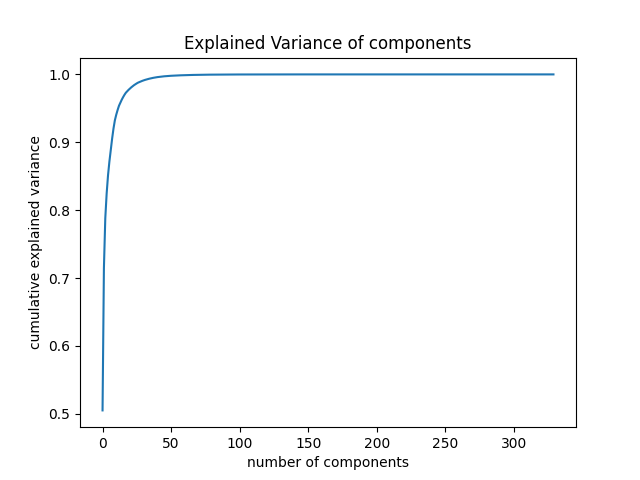
\includegraphics[width=1\linewidth]{figures/pca.png}
		  \caption{Features explaining variance}
		  \label{fig:pca}
	\end{subfigure}
	\begin{subfigure}[h]{.32\textwidth}
	  \centering
	  	
		{
		\centering\settowidth\rotheadsize{\bfseries(our proposal)}
		\renewcommand\theadalign{cl}\renewcommand\cellalign{cl}
		\renewcommand\theadfont{\bfseries}
		\renewcommand\tabcolsep{4pt}\renewcommand\arraystretch{1.25}
		% Make this a bit smaller so it will fit on a page.  Still looks a bit nasty in that it extends to the edge of the page.
		% It's that PCA line that is the trouble, as the values are just too long
		\footnotesize
		
		\begin{longtable}[c]{
		    |l |*{12}{c |} }%
		    \hline
		    %\diagbox[height=1.2\rotheadsize, width=\dimexpr\eqboxwidth{AB}+2\tabcolsep\relax]%
		    %{\raisebox{1.2ex}{Feature}}{\raisebox{-5ex}{Feature}} &
		    {\textbf{Feature}} & {\textbf{Importance Rank}}\\
		    %\rothead{Tool X\\\mbox{(our proposal)}}\\
		    \hline
			hue                      &     0.505089 \\
			saturation\_mean          &     0.209646 \\
			in\_phase                 &     0.073444 \\
			cb\_mean                  &     0.036392 \\
			hog\_stddev               &     0.026874 \\
			hog\_mean                 &     0.020135 \\
			hog\_variance             &     0.017359 \\
			greyscale\_homogeneity\_0  &     0.016602 \\
			greyscale\_homogeneity\_45 &     0.014872 \\
			greyscale\_homogeneity\_90 &     0.012052 \\	    
		    
		    \hline
		    %\caption{Feature Importance Ranks using RFE with a Random Forest Classifier}
		    %\label{fig:random-forest}
		  \end{longtable}
		 }
	  \caption{PCA Variances}
  %\label{fig:sub2}
	\end{subfigure}
\caption{Principal Component Analysis of Features}
\label{fig:pca}
\end{figure}




 
  Given these observations, we can use these parameters for our training and prediction:
 \begin{itemize}
	\item{The length/width ratio}
	\item{The shape index}
	\item{The YIQ in-phase mean}
	\item{The distance from the cropline}
\end{itemize}

Plotting these attributes along with their classification via Logistic Regression yields Figure~\ref{fig:factors}. This plot shows that items correctly classified as weeds are are tightly grouped. Vegetation correctly classified as crop shows a somewhat looser, but still quite evident grouping.
 \begin{figure}[H]
	\centering
	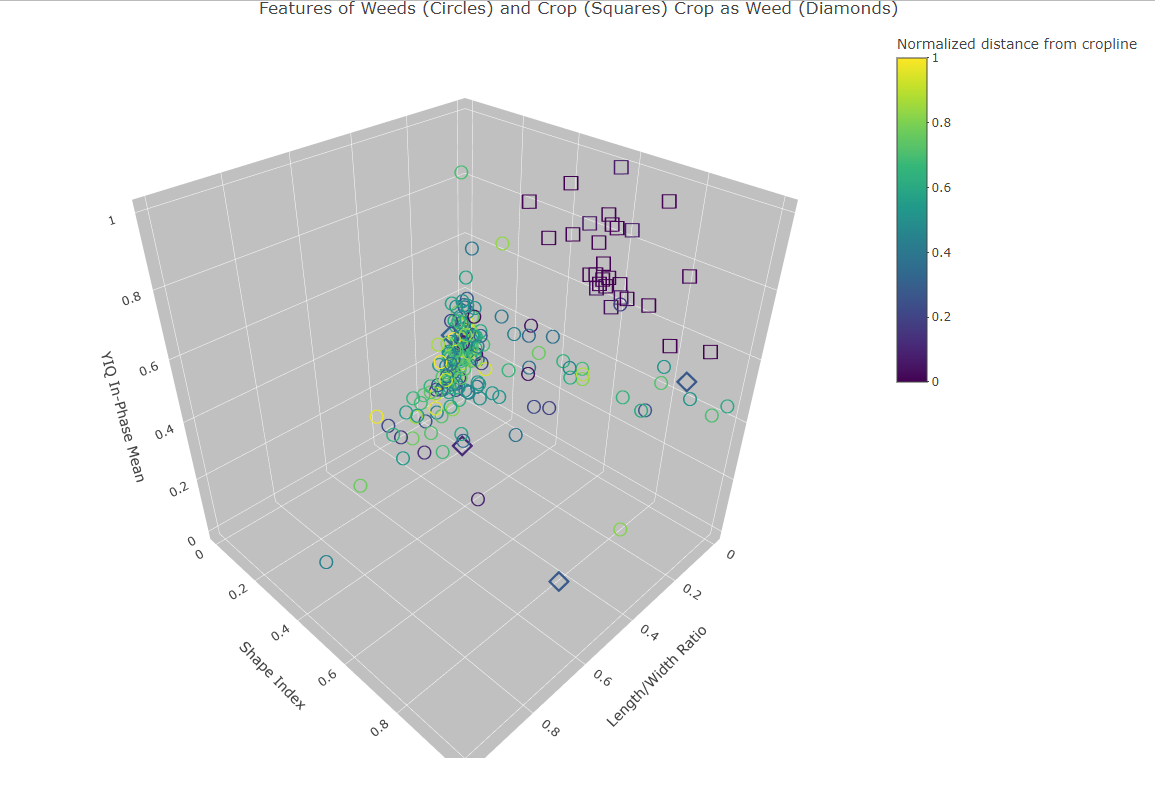
\includegraphics[width=0.9\linewidth]{./figures/plot-factors.png}
	\caption[Factors selected for discrimination]{A plot of the four factors selected with the shape noting the true classification of the blob. In this graph the factors selected occupy space and color, with the shape of the object noting the classification.}
	\label{fig:factors}
\end{figure}
  
\section{Classification}
Before delving into the details of classification, it is worthwhile to consider an aspect of the images that must be considered in classification: most of the vegetation appearing is crop; very few of the plants are actually weeds. While the scarcity of weeds is certainly a good thing for farmer, that scarcity has some odd effects on the data. If a dataset contains attributes of 1000 crop plants and 100 weeds, for instance, a 99\% accurate classifier is easily achieved by simply classifying every plant as a crop (a reminder than overall accuracy claims are almost always dubious, and are rightly treated as suspect -- here, a high accuracy claim is perilously close to useless). \citeauthor{Fernandez2018-fw}  deals with the topic of imbalanced data (sets where a majority class is seen several times more often as a minority class) at length in his book on the subject, outlining details of solutions to this imbalance between majority (crop) and minority (weed) classes: sampling, algorithmic changes, and cost-sensitive learning \parencite{Fernandez2018-fw}. Sampling corrections fall into two categories: under sample the majority to lower the number in the final set or over sample the minority class to lower the imbalance ratio. While over sampling the minority class has a set of problems that are best summarized as \textit{``there may be only a few samples to even use -- we need to synthesize more''}, under sampling the majority class has its own set of problems that comes down to choosing the \textit{best} samples that are representative of the class. Synthesizing new instances of the minority class and the using those in an over sampling technique are frequently addressed by using Synthetic Minority Oversampling Technique (SMOTE). Numerous variants of SMOTE exist as do alternatives\footnote{\citeauthor{Fernandez2018-fw} discuss the details of SMOTE, SMOTE variants and extensions, and alternative approaches (such as ADASYN, which addresses linear dependencies between synthetic data points) in their book on imbalanced learning \parencite[p.~101]{Fernandez2018-fw}. While the details of these techniques is beyond the scope of this paper, the pre-processing techniques described in that publication will be used in this problem space.} While choosing between the two techniques (over-sample minority or under-sample majority) is frequently done, applying a hybrid technique of both reducing the majority and generating new minority class samples to address the imbalance is also performed. Here, \citeauthor{Fernandez2018-fw} describe two techniques: SMOTE+Tomek Link, and SMOTE+ENN. Tomek links exist between instances of different classes that are close to each other. Removing the majority class instances subsequently increases the distance separating the two classes. The Edited Nearest Neighbor (ENN) algorithm removes instances whose class label differs from two of three nearest neighbors.
Cost sensitive learning formalizes the concept that some mistakes are more costly than others. Consider the case of weed control: mistakenly stating that a weed is a crop and not treating it is not immediately costly, as no vegetation is altered, but mistakenly stating that a crop is a weed and then applying a treatment is immediately costly, as marketable vegetation has been damaged.

Using the subset of the parameters identified in the previous section, various approaches were used in classifying the objects isolated in the images and detailed in Table~\ref{fig:learning}. The feature sets were split into a 80\%/20\% for these results: 

{\renewcommand{\arraystretch}{2}%
\begin{table}[H]
	\centering
    \caption{Learning Results}
    \label{fig:learning}
    \begin{tabular}{  l  p{4cm}  p{5cm} }
     %\begin{tabular}{  l  p{3.4cm}  p{3.4cm} }
        \toprule
\textbf{Method}      
& \textbf{Train}   
& \textbf{Test} \\\midrule
Random Forest      
& 1.0
& 0.986 \\\hline
Logistic Regression
& 0.9790       
& 0.9787 \\\hline
Decision Tree
& 1.0
& 0.96 \\\hline
Boosted Gradient     
& 1.0
& 0.957 \\\hline
KNN     
& $1.0$                    
& $0.86$ \\\hline
        \bottomrule
    \end{tabular}
\end{table}

For this sample dataset, all approaches with the exception of KNN yield commercially acceptable results if accuracy were the only criterion used in evaluation. However this case must consider two other criteria that are important, but beyond the scope of this document:
\begin{itemize}
\item{The computational cost of achieving each result. The prediction will be done in real-time under field conditions\footnote{And on a GPU, not on a CPU as was done here} While a result of an approach yielding results above 98\% may sound impressive, if that prediction using logistic regression takes a few hundred milliseconds and a decision tree takes well under 100 milliseconds, it may be the case that using that logistic regression in practice is not viable.\footnote{Some context is probably needed here. This prediction will be done as a tractor is moving along, and the time spent on prediction is part of an overall time budget that will ultimately limit the forward speed of the tractor. 2 MPH is commercially viable. 1 MPH is not.}}
\item{The cost of misclassifying a crop as a weed has very real dollar cost, as the subsequent killing of that plant would negatively impact the total crop suitable for sale. The cost of classifying a weed as a crop (and thus not flagging it for treatment) is much lower. While it may have modest financial impact, as leaving the weed in place allows it to take resources away from marketable vegetation (water, fertilizer), the impact of doing so may be acceptable in most instances.}
\end{itemize}
 
Misclassification rates where crop is identified as a weed is the most pressing concern here, so it is worthwhile evaluating the performance of these approaches with the goal of minimizing that class of misclassification while maximizing the correct classification of weeds as weeds. Figure~\ref{fig:classification-rates} addresses this goal by showing percentages of correct and incorrect classifications. While there several approaches showed quite similar acceptable  results (SVM, Random Forest, and Logistic Regression) and three approaches with unacceptable results (KNN, Boosted Gradient, and Decision Tree). While it is likely the case that the unacceptable approaches can be optimized to the point that their results would migrate them to the acceptable category, this paper will concentrate only on the approaches will acceptable results.

\begin{figure}[h]
	\centering
	\includegraphics[width=0.7\linewidth]{./figures/classification-rates.png}
	\caption[Misclassification rates of various algorithms]{The correct and misclassification rates of various algorithms are shown here. While an overall accuracy of 95.7\% may sound impressive for the Boosted Gradient algorithm (See Table~\ref{fig:learning}), considering the salient misclassification and correct classification rates, 24.1\% and 98.6\%, respectively, that algorithm does not support the accuracy needed in this use case.}
	\label{fig:classification-rates}
\end{figure}

Figure~\ref{fig:classified} shows an annotated classification result. In this figure, we see desirable (crop) bounded by a green box, and undesirable (not crop) bounded in red. The blue box bounds vegetation for which we can't reliably determine its class. Computations that depend on an unimpeded view of the vegetation ({\it length/width ratio}, for instance) can't be reliably performed, so classification of elements that are not fully captured are not classified. Some color computations could be, but may not be as representative as required. The {\it hue} value, for example, is the mean value across the entire plant, and the hue may not be consistent across the entire plant. The portion that is visible may not be representative of the plant as a whole.

\begin{figure}[H]
	\centering
	\includegraphics[width=0.7\linewidth]{./figures/classified-result.jpg}
	\caption[A classified and annotated image]{A classified result. Desirable vegetation is bounded in green and undesirable in red. Note that this image also demonstrates a commonly encountered problem, that of overlapping vegetation. In the lower left of the green bounding box there is a weed that is overlapped by crop vegetation. In this case, however, the weed's proximity to the crop makes treatment problematic in that doing so represents a risk of producing crop damage.}
	\label{fig:classified}
\end{figure}


\section{Treatment Maps}

\section{Future Work}

\newpage
\section{References}
\printbibliography[heading=none]

%\cite{Wirth2004-li}
\end{document}

